\documentclass[10pt]{article}
\usepackage[verbose, a4paper, hmargin=2.5cm, vmargin=2.5cm]{geometry}

\usepackage{fontspec}
\usepackage{ctex}
\usepackage{paratype}

\usepackage{amsmath}
\usepackage{amssymb}
\usepackage{amsfonts}
\usepackage{esint}
\usepackage{stmaryrd}

\usepackage[mathbf=sym]{unicode-math}
\setmainfont{STIX Two Text}
\setmathfont{STIX Two Math}

\setsansfont{Arial}
\setmonofont{Courier New}

\usepackage{makecell}
\usepackage{wasysym}
\usepackage{pifont}
\usepackage[export]{adjustbox}
\usepackage{graphicx}
\usepackage{mdframed}
\usepackage{booktabs,array,multirow}
\usepackage{tabularx}
\usepackage{hyperref}
\hypersetup{colorlinks=true, linkcolor=blue, filecolor=magenta, urlcolor=cyan,}
\urlstyle{same}
\usepackage[most]{tcolorbox}
\definecolor{mygray}{RGB}{240,240,240}
\tcbset{
  colback=mygray,
  boxrule=0pt,
}
\newtcolorbox{problem}[1][]{
  colback=white,
  colframe=black,
  boxrule=0.5mm,
  title=题目,
  fonttitle=\bfseries,
  #1
}
\graphicspath{ {./images/} }
\newcommand{\HRule}{\begin{center}\rule{0.9\linewidth}{0.2mm}\end{center}}
\newcommand{\customfootnote}[1]{
  \let\thefootnote\relax\footnotetext{#1}
}
\newcommand{\lt}{\mathrel{<}}
\newcommand{\gt}{\mathrel{>}}
\newcommand*\circled[1]{\tikz[baseline=(char.base)]{\node[shape=circle,draw,inner sep=1.5pt] (char) {\small #1};}}
\setcounter{MaxMatrixCols}{256}
\begin{document}
Step 4: Determine the Curve's Shape.

Rearranging the equation:

\[
c\left( s\right)  - {C}_{0} =  - \frac{1}{{\kappa }_{0}}N\left( s\right)
\]

Now, take the norm (length) of both sides:

\[
\begin{Vmatrix}{c\left( s\right)  - {C}_{0}}\end{Vmatrix} = \begin{Vmatrix}{-\frac{1}{{\kappa }_{0}}N\left( s\right) }\end{Vmatrix}
\]

Since \({\kappa }_{0} > 0\) is constant and \(N\left( s\right)\) is a unit vector \(\left( {\parallel N\left( s\right) \parallel  = 1}\right)\) :

\[
\begin{Vmatrix}{c\left( s\right)  - {C}_{0}}\end{Vmatrix} = \frac{1}{{\kappa }_{0}}\parallel N\left( s\right) \parallel  = \frac{1}{{\kappa }_{0}}
\]

Let \(R = 1/{\kappa }_{0}\) . We have:

\[
\begin{Vmatrix}{c\left( s\right)  - {C}_{0}}\end{Vmatrix} = R
\]

This equation defines a set of points \(c\left( s\right)\) whose distance to the fixed point \({C}_{0}\) is the constant \(R\) . By definition, the curve \(c\left( s\right)\) is a circle of radius \(R = 1/{\kappa }_{0}\) centered at \({C}_{0}\) .

Through the proof, we could see that a point on the circle with the curvature and the tangent direction could determine the circle and the radius \(R = \frac{1}{\kappa }\) . Hence, under the dilation \(x \mapsto  {rx}\) , the new radius \({R}^{\prime } = {rR}\) and the new curvature \({\kappa }^{\prime } = \frac{1}{{R}^{\prime }} = \frac{1}{rR} = \frac{1}{r}\kappa\) .

\begin{problem}[title=PROBLEM 2 (5 POINTS)]
Compute the curvature of an ellipse. Where does it reach its maxima and minima? Also try to compute the length of an ellipse (you can stop once you have an integral you cannot solve).
\end{problem}

Solution. 1. Parametrization of the Ellipse A standard parametrization for an ellipse is \(c\left( t\right)  = \left( {a\cos t,b\sin t}\right)\) , where \(t \in  \left\lbrack  {0,{2\pi }}\right\rbrack  ,a,b > 0\) .

2. Derivatives

\[
\dot{c}\left( t\right)  = \left( {-a\sin t,b\cos t}\right)
\]

\[
\ddot{c}\left( t\right)  = \left( {-a\cos t, - b\sin t}\right)
\]

3. Curvature Computation The curvature formula is \(\kappa \left( t\right)  = \frac{1}{v{\left( t\right) }^{2}}\sqrt{\parallel \ddot{c}\left( t\right) {\parallel }^{2} - \dot{v}{\left( t\right) }^{2}}\) .

\[
\kappa \left( t\right)  = \frac{ab}{{\left( {a}^{2}{\sin }^{2}t + {b}^{2}{\cos }^{2}t\right) }^{3/2}}.
\]

4. Maxima and Minima of Curvature To find the extrema of \(\kappa \left( t\right)\) , we need to find the extrema of the denominator \(D\left( t\right)  = {\left( {a}^{2}{\sin }^{2}t + {b}^{2}{\cos }^{2}t\right) }^{3/2}\) . Since \(f\left( x\right)  = {x}^{3/2}\) is a monotonic increasing function for \(x > 0\) , finding the extrema of \(D\left( t\right)\) is equivalent to finding the extrema of its base \(g\left( t\right)  = {a}^{2}{\sin }^{2}t + {b}^{2}{\cos }^{2}t\) .

\(g\left( t\right)  = {a}^{2}{\sin }^{2}t + {b}^{2}\left( {1 - {\sin }^{2}t}\right)  = \left( {{a}^{2} - {b}^{2}}\right) {\sin }^{2}t + {b}^{2}.\)

\begin{itemize}\relax
\item\relax Minimum of \(g\left( t\right)\) : Occurs when \({\sin }^{2}t\) is minimized (if \({a}^{2} > {b}^{2}\) ) or maximized (if \({a}^{2} < {b}^{2}\) ).
\end{itemize}

\begin{itemize}\relax
\item\relax Assume \(a > b\) (major axis on \(x\) -axis). \(g\left( t\right)\) is minimized when \({\sin }^{2}t = 0\) , i.e., \(t = 0,\pi\) . \({g}_{\min } = {b}^{2}\) . \({\kappa }_{\max } = \frac{ab}{{\left( {b}^{2}\right) }^{3/2}} = \frac{a}{{b}^{2}}\) . These occur at \(c\left( 0\right)  = \left( {a,0}\right)\) and \(c\left( \pi \right)  = \left( {-a,0}\right)\) (the ends of the major axis).
\end{itemize}

\begin{itemize}\relax
\item\relax Maximum of \(g\left( t\right)\) : Occurs when \({\sin }^{2}t = 1\) , i.e., \(t = \pi /2,{3\pi }/2.\;{g}_{\max } = \left( {{a}^{2} - {b}^{2}}\right)  \cdot  1 + {b}^{2} = {a}^{2}\) . \({\kappa }_{\min } = \frac{ab}{{\left( {a}^{2}\right) }^{3/2}} = \frac{b}{{a}^{2}}\) . These occur at \(c\left( {\pi /2}\right)  = \left( {0,b}\right)\) and \(c\left( {{3\pi }/2}\right)  = \left( {0, - b}\right)\) (the ends of the minor axis).
\end{itemize}

Conclusion: The curvature is **maximum** at the ends of the minor axis and **minimum** at the ends of the major axis (assuming \(a > b\) ).

5. Arc Length Computation The length \(L\left( c\right)\) is given by \(L\left( c\right)  = {\int }_{0}^{2\pi }\parallel \dot{c}\left( t\right) \parallel \mathrm{d}t\) .

\[
L\left( c\right)  = {\int }_{0}^{2\pi }\sqrt{{a}^{2}{\sin }^{2}t + {b}^{2}{\cos }^{2}t}\mathrm{\;d}t
\]

If we factor out \(a\) and let \({e}^{2} = 1 - {\left( b/a\right) }^{2}\) (the eccentricity squared), we get:

\[
L\left( c\right)  = {\int }_{0}^{2\pi }a\sqrt{{\sin }^{2}t + {\left( b/a\right) }^{2}{\cos }^{2}t}\mathrm{\;d}t
\]

\[
L\left( c\right)  = {\int }_{0}^{2\pi }a\sqrt{{\cos }^{2}t + \left( {1 - {e}^{2}}\right) {\sin }^{2}t}\mathrm{\;d}t
\]

\[
L\left( c\right)  = {4a}{\int }_{0}^{\pi /2}\sqrt{1 - {e}^{2}{\sin }^{2}t}\mathrm{\;d}t.
\]

The integral \(E\left( e\right)  = {\int }_{0}^{\pi /2}\sqrt{1 - {e}^{2}{\sin }^{2}t}\mathrm{\;d}t\) is the complete elliptic integral of the second kind. It cannot be solved in terms of elementary functions.

\begin{problem}[title=PROBLEM 3 (7 POINTS)]
Let \(c : \left\lbrack  {a,b}\right\rbrack   \rightarrow  {\mathbb{R}}^{2}\) be a regular curve given in polar coordinates by a function \(r = r\left( \phi \right)\) , where \(r\) is the distance from the origin and \(\phi  \in  \left\lbrack  {a,b}\right\rbrack\) is the angle with the \(x\) -axis. So, in cartesian coordinates we have

\[
c\left( \phi \right)  = \left( \begin{array}{l} r\left( \phi \right) \cos \phi \\  r\left( \phi \right) \sin \phi  \end{array}\right) .
\]

Show that the length of \(c\) is given by

\[
L\left( c\right)  = {\int }_{a}^{b}\sqrt{r{\left( \phi \right) }^{2} + {r}^{\prime }{\left( \phi \right) }^{2}}\mathrm{\;d}\phi
\]

and that its curvature is given by

\[
\kappa \left( \phi \right)  = \frac{r{\left( \phi \right) }^{2} + 2{r}^{\prime }{\left( \phi \right) }^{2} - r\left( \phi \right) {r}^{\prime \prime }\left( \phi \right) }{{\left( r{\left( \phi \right) }^{2} + {r}^{\prime }{\left( \phi \right) }^{2}\right) }^{\frac{3}{2}}}
\]
\end{problem}

Solution. 1. Derivatives Let \(r = r\left( \phi \right)\) and \({r}^{\prime } = {r}^{\prime }\left( \phi \right)  = \mathrm{d}r/\mathrm{d}\phi\) . The curve is \(c\left( \phi \right)  = \left( {x\left( \phi \right) ,y\left( \phi \right) }\right)\) where \(x\left( \phi \right)  = r\cos \phi\) and \(y\left( \phi \right)  = r\sin \phi .\)

\[
\dot{c}\left( \phi \right)  = \frac{\mathrm{d}c}{\mathrm{\;d}\phi } = \left( \begin{array}{l} {r}^{\prime }\cos \phi  - r\sin \phi \\  {r}^{\prime }\sin \phi  + r\cos \phi  \end{array}\right)
\]

\[
\ddot{c}\left( \phi \right)  = \frac{{\mathrm{d}}^{2}c}{\mathrm{\;d}{\phi }^{2}} = \left( \begin{matrix} \left( {{r}^{\prime \prime }\cos \phi  - {r}^{\prime }\sin \phi }\right)  - \left( {{r}^{\prime }\sin \phi  + r\cos \phi }\right) \\  \left( {{r}^{\prime \prime }\sin \phi  + {r}^{\prime }\cos \phi }\right)  + \left( {{r}^{\prime }\cos \phi  - r\sin \phi }\right)  \end{matrix}\right)
\]

\[
= \left( \begin{array}{l} {r}^{\prime \prime }\cos \phi  - 2{r}^{\prime }\sin \phi  - r\cos \phi \\  {r}^{\prime \prime }\sin \phi  + 2{r}^{\prime }\cos \phi  - r\sin \phi  \end{array}\right)
\]

2. Arc Length \(L\left( c\right)\) The length formula is \(L\left( c\right)  = {\int }_{a}^{b}\parallel \dot{c}\left( \phi \right) \parallel \mathrm{d}\phi\) .

\[
\parallel \dot{c}{\parallel }^{2} = {\left( {r}^{\prime }\cos \phi  - r\sin \phi \right) }^{2} + {\left( {r}^{\prime }\sin \phi  + r\cos \phi \right) }^{2}
\]

\[
= \left( {{r}^{\prime 2}{\cos }^{2}\phi  - {2r}{r}^{\prime }\cos \phi \sin \phi  + {r}^{2}{\sin }^{2}\phi }\right)  + \left( {{r}^{\prime 2}{\sin }^{2}\phi  + {2r}{r}^{\prime }\sin \phi \cos \phi  + {r}^{2}{\cos }^{2}\phi }\right)
\]

\[
= {r}^{\prime 2}\left( {{\cos }^{2}\phi  + {\sin }^{2}\phi }\right)  + {r}^{2}\left( {{\sin }^{2}\phi  + {\cos }^{2}\phi }\right)
\]

\[
= {r}^{2} + {r}^{\prime 2}\text{ . }
\]

Therefore,

\[
L\left( c\right)  = {\int }_{a}^{b}\sqrt{r{\left( \phi \right) }^{2} + {r}^{\prime }{\left( \phi \right) }^{2}}\mathrm{\;d}\phi .
\]

3. Curvature \(\kappa \left( \phi \right)\) The curvature formula is \(\kappa \left( t\right)  = \frac{1}{v{\left( t\right) }^{2}}\sqrt{\parallel \ddot{c}\left( t\right) {\parallel }^{2} - \dot{v}{\left( t\right) }^{2}}\) .

\[
\kappa \left( \phi \right)  = \frac{r{\left( \phi \right) }^{2} + 2{r}^{\prime }{\left( \phi \right) }^{2} - r\left( \phi \right) {r}^{\prime \prime }\left( \phi \right) }{{\left( r{\left( \phi \right) }^{2} + {r}^{\prime }{\left( \phi \right) }^{2}\right) }^{\frac{3}{2}}}.
\]

\section*{1.2 EXAM-QUALIFYING PROBLEMS}

\begin{problem}[title=PROBLEM 4 (4 POINTS)]
Try to find the arc length parametrization of a parabola. If you cannot find a closed form solution, explain why.
\end{problem}

Solution. 1. Parabola Parametrization A standard parabola is \(y = {x}^{2}\) , which can be parametrized by \(c\left( t\right)  = \left( {t,{t}^{2}}\right) .\)

2. Arc Length Function \(s\left( t\right)\)

\[
\dot{c}\left( t\right)  = \left( {1,{2t}}\right)
\]

\[
\parallel \dot{c}\left( t\right) \parallel  = \sqrt{1 + 4{t}^{2}}
\]

The arc length function starting from \(t = 0\) is:

\[
s\left( t\right)  = {\int }_{0}^{t}\parallel \dot{c}\left( u\right) \parallel \mathrm{d}u = {\int }_{0}^{t}\sqrt{1 + 4{u}^{2}}\mathrm{\;d}u.
\]

3. Integration This integral can be solved using a trigonometric or hyperbolic substitution. Let \({2u} = \tan \theta\) (or \({2u} = \sinh v\) ). Using the hyperbolic substitution \({2u} = \sinh v\) , so \(2\mathrm{\;d}u = \cosh v\mathrm{\;d}v\) :

\[
s\left( t\right)  = {\int }_{u = 0}^{u = t}\sqrt{1 + {\sinh }^{2}v} \cdot  \frac{1}{2}\cosh v\mathrm{\;d}v = \frac{1}{2}{\int }_{u = 0}^{u = t}{\cosh }^{2}v\mathrm{\;d}v.
\]

Using the half-angle formula \({\cosh }^{2}v = \frac{1 + \cosh {2v}}{2}\) :

\[
s\left( t\right)  = \frac{1}{4}{\int }_{u = 0}^{u = t}\left( {1 + \cosh {2v}}\right) \mathrm{d}v = \frac{1}{4}{\left\lbrack  v + \frac{1}{2}\sinh 2v\right\rbrack  }_{u = 0}^{u = t}.
\]

Substituting back \(v = \operatorname{arsinh}\left( {2u}\right)\) and \(\sinh {2v} = 2\sinh v\cosh v = 2\left( {2u}\right) \sqrt{1 + 4{u}^{2}}\) :

\[
s\left( t\right)  = \frac{1}{4}{\left\lbrack  \operatorname{arsinh}\left( 2u\right)  + 2u\sqrt{1 + 4{u}^{2}}\right\rbrack  }_{0}^{t}
\]

\[
s\left( t\right)  = \frac{1}{4}\left( {\operatorname{arsinh}\left( {2t}\right)  + {2t}\sqrt{1 + 4{t}^{2}}}\right) .
\]

Since \(\operatorname{arsinh}\left( x\right)  = \ln \left( {x + \sqrt{{x}^{2} + 1}}\right)\) , we have:

\[
s\left( t\right)  = \frac{1}{4}\left( {\ln \left( {{2t} + \sqrt{4{t}^{2} + 1}}\right)  + {2t}\sqrt{1 + 4{t}^{2}}}\right) .
\]

\begin{problem}[title=PROBLEM 5 (5 POINTS)]
Let \(c : I \rightarrow  {\mathbb{R}}^{2}\) be a unit-speed curve. An osculating circle to \(c\) at \(c\left( {t}_{0}\right)\) (for some \({t}_{0} \in  I\) ) is a circle that touches \(c\) at \(c\left( {t}_{0}\right)\) up to second order. In other words, if the circle is parametrized by a unit-speed curve \(\sigma  : I \rightarrow  {\mathbb{R}}^{2}\) then the Taylor expansion of \(\sigma\) around 0 coincides with the Taylor expansion of \(c\) around \({t}_{0}\) up to second order:

\[
\sigma \left( 0\right)  = c\left( {t}_{0}\right) ,\;\dot{\sigma }\left( 0\right)  = \dot{c}\left( {t}_{0}\right) \;\text{ and }\;\ddot{\sigma }\left( 0\right)  = \ddot{c}\left( {t}_{0}\right)
\]

Show that if \(\ddot{c}\left( {t}_{0}\right)  \neq  0\) then there exists an osculating circle to \(c\) at \(c\left( {t}_{0}\right)\) . Give an explicit parametrization \(\sigma\) of the osculating circle. Hint: Use the fact that \(T\left( {t}_{0}\right)\) and \(N\left( {t}_{0}\right)\) form an orthonormal basis.
\end{problem}

Solution. We have a point on the circle, the tangent direction and the curvature. These information could determine our circle uniquely. For details, see 12. The simplest form for parametrization is: Let \(R = 1/\left| {\kappa }_{0}\right| .\)

\[
C = c\left( {t}_{0}\right)  + \frac{1}{{\kappa }_{0}}N\left( {t}_{0}\right)
\]

\[
\sigma \left( s\right)  = C + R\left\lbrack  {\cos \left( \frac{s}{R}\right) \left( {-\operatorname{sgn}\left( {\kappa }_{0}\right) N\left( {t}_{0}\right) }\right)  + \sin \left( \frac{s}{R}\right) T\left( {t}_{0}\right) }\right\rbrack
\]

where \(T\left( {t}_{0}\right)  = \dot{c}\left( {t}_{0}\right)\) and \(N\left( {t}_{0}\right)  = \frac{1}{{\kappa }_{0}}\ddot{c}\left( {t}_{0}\right)\) .

\section*{2 Homework 2}

\section*{2.1 GRADE-INFLUENCING PROBLEMS}

PROBLEM 1 (5 POINTS)

Reparametrize the curve \(c\left( t\right)  = \left( {\cosh t,\sinh t,t}\right)\) by arc length.

Solution. First, we calculate the speed of the curve \(c\left( t\right)\) :

\[
\dot{c}\left( t\right)  = \left( {\sinh t,\cosh t,1}\right) .
\]

The speed \(v\left( t\right)  = \parallel \dot{c}\left( t\right) \parallel\) is:

\[
v\left( t\right)  = \sqrt{{\left( \sinh t\right) }^{2} + {\left( \cosh t\right) }^{2} + {1}^{2}} = \sqrt{{\sinh }^{2}t + {\cosh }^{2}t + 1}.
\]

Using the identity \({\cosh }^{2}t - {\sinh }^{2}t = 1\) , we have \({\cosh }^{2}t = 1 + {\sinh }^{2}t\) , so

\[
v\left( t\right)  = \sqrt{{\sinh }^{2}t + \left( {1 + {\sinh }^{2}t}\right)  + 1} = \sqrt{2{\sinh }^{2}t + 2} = \sqrt{2\left( {{\sinh }^{2}t + 1}\right) } = \sqrt{2{\cosh }^{2}t} = \sqrt{2}\cosh t.
\]

The arc length function \(s\left( t\right)\) starting at \({t}_{0} = 0\) is:

\[
s\left( t\right)  = {\int }_{0}^{t}v\left( \tau \right) {d\tau } = {\int }_{0}^{t}\sqrt{2}\cosh {\tau d\tau } = \sqrt{2}{\left\lbrack  \sinh \tau \right\rbrack  }_{0}^{t} = \sqrt{2}\sinh t.
\]

To reparametrize the curve, we need to find the inverse function \(t\left( s\right)\) :

\[
s = \sqrt{2}\sinh t \Rightarrow  \sinh t = \frac{s}{\sqrt{2}} \Rightarrow  t\left( s\right)  = \operatorname{arsinh}\left( \frac{s}{\sqrt{2}}\right) .
\]

Using the identity \(\cosh t = \sqrt{1 + {\sinh }^{2}t}\) , we have

\[
\cosh t = \sqrt{1 + {\left( \frac{s}{\sqrt{2}}\right) }^{2}} = \sqrt{1 + \frac{{s}^{2}}{2}} = \frac{\sqrt{2 + {s}^{2}}}{\sqrt{2}}.
\]

Substituting \(t\left( s\right)\) back into \(c\left( t\right)\) , the reparametrized curve \(\widetilde{c}\left( s\right)\) is:

\[
\widetilde{c}\left( s\right)  = c\left( {t\left( s\right) }\right)  = \left( {\frac{\sqrt{2 + {s}^{2}}}{\sqrt{2}},\frac{s}{\sqrt{2}},\operatorname{arsinh}\left( \frac{s}{\sqrt{2}}\right) }\right) .
\]

\begin{problem}[title=PROBLEM 2 (6 POINTS)]
Let \(c : \left\lbrack  {a,b}\right\rbrack   \rightarrow  {\mathbb{R}}^{2}\) be a regular curve and \(\widetilde{c} = c \circ  \varphi\) its reparametrization by arc length. As in the lecture, the curvature of \(c\) is defined by \(\kappa \left( t\right)  = \widetilde{\kappa }\left( {{\varphi }^{-1}\left( t\right) }\right)\) , where \(\widetilde{\kappa }\left( s\right)  = \begin{Vmatrix}{\frac{{d}^{2}\widetilde{c}}{d{s}^{2}}\left( s\right) }\end{Vmatrix}\) is the curvature of \(\widetilde{c}\left( s\right)\) . Denote the speed of \(c\) by \(v\left( t\right)  = \parallel \dot{c}\left( t\right) \parallel\) . Prove that

\[
\kappa \left( t\right)  = \frac{1}{v{\left( t\right) }^{2}}\sqrt{\parallel \ddot{c}\left( t\right) {\parallel }^{2} - {\left( \dot{v}\left( t\right) \right) }^{2}}
\]

where \(\dot{v}\left( t\right)  = \frac{\mathrm{d}v\left( t\right) }{\mathrm{d}t}\) .
\end{problem}

Solution. By definition, \(\kappa \left( t\right)  = \widetilde{\kappa }\left( {{\varphi }^{-1}\left( t\right) }\right)  = \widetilde{\kappa }\left( s\right)  = \parallel \widetilde{\mathbf{n}}\left( s\right) \parallel\) . We have

\[
\widetilde{\mathbf{t}}\left( s\right)  = \frac{\mathrm{d}\widetilde{c}}{\mathrm{\;d}s} = \frac{\mathrm{d}\varphi }{\mathrm{d}s} \cdot  \frac{\mathrm{d}c}{\mathrm{\;d}t}.
\]

Note that \(\widetilde{\mathbf{t}}\) is a unit vector. Without loss of generality, we can assume that

\[
\frac{\mathrm{d}\varphi }{\mathrm{d}s} = \frac{1}{\parallel \dot{c}\left( t\right) \parallel }.
\]

Through further computation, we have

\[
\widetilde{\mathbf{n}}\left( s\right)  = \frac{\mathrm{d}\widetilde{\mathbf{t}}}{\mathrm{d}s} = {\left( \frac{\mathrm{d}\varphi }{\mathrm{d}s}\right) }^{2} \cdot  \frac{{\mathrm{d}}^{2}c}{\mathrm{\;d}{t}^{2}} + \frac{{\mathrm{d}}^{2}\varphi }{\mathrm{d}{s}^{2}} \cdot  \frac{\mathrm{d}c}{\mathrm{\;d}t}.
\]

Observe that \(\widetilde{\mathbf{n}}\left( s\right)\) is orthogonal to \(\dot{c}\left( t\right)\) . Hence,

\[
\begin{Vmatrix}{\widetilde{\mathbf{n}}\left( s\right) }\end{Vmatrix} = \sqrt{\begin{Vmatrix}{{\left( \frac{\mathrm{d}\varphi }{\mathrm{d}s}\right) }^{2} \cdot  \frac{{\mathrm{d}}^{2}c}{\mathrm{\;d}{t}^{2}}}\end{Vmatrix}/{\left. \begin{Vmatrix}\frac{{\mathrm{d}}^{2}\varphi }{\mathrm{d}{s}^{2}} \cdot  \frac{\mathrm{d}c}{\mathrm{\;d}t}\end{Vmatrix}\right| }^{2}} = \frac{1}{v{\left( t\right) }^{2}}\sqrt{\parallel \ddot{c}\left( t\right) {\parallel }^{2} - {\left( \dot{v}\left( t\right) \right) }^{2}}.
\]

\begin{problem}[title=PROBLEM 3 (7 POINTS)]
A closed planar curve \(c\) is said to have constant width \(w\) if the distance between every pair of parallel tangent lines of \(c\) is always \(w\) . Suppose that \(c : \left\lbrack  {0,T}\right\rbrack   \rightarrow  {\mathbb{R}}^{2}\) is a unit-speed loop with curvature \(\kappa  > 0\) and constant width \(w\) .

In any pair of parallel tangent lines, one of the two lines will necessarily touch the curve at a point \(c\left( t\right)\) . The other tangent line touches the curve at another point \({c}^{op}\left( t\right)\) , called the opposite point of \(c\left( t\right)\) .

1. Show that \({c}^{op}\left( t\right)  = c\left( t\right)  + {wN}\left( t\right)\) , where \(N\left( t\right)\) is the unit normal vector of \(c\) at \(t\) .

2. Let \(\kappa \left( t\right)\) be the curvature of \(c\) at \(t\) , and let \({\kappa }^{op}\left( t\right)\) be the curvature of \({c}^{op}\left( t\right)\) (the latter seen as an independent curve in \({\mathbb{R}}^{2}\) ). Prove that \(\frac{1}{\kappa \left( t\right) } + \frac{1}{{\kappa }^{op}\left( t\right) } = w\) .
\end{problem}

Solution. Part 1: Show that \({c}^{op}\left( t\right)  = c\left( t\right)  + {wN}\left( t\right)\)

Using the Frenet-Serret frame, it is possible to write \({c}^{op}\left( t\right)  = c\left( t\right)  + A\left( t\right) T\left( t\right)  + B\left( t\right) N\left( t\right)\) , where \(\{ c\left( t\right) ;T\left( t\right) ,N\left( t\right) \}\) is the Frenet-Serret frame associated with \(c\left( t\right)\) . We need to verify several conditions.

\begin{itemize}\relax
\item\relax \({\dot{c}}^{op}\left( t\right)\) is parallel to \(T\left( t\right)\)
\end{itemize}

\begin{itemize}\relax
\item\relax The distance between every pair of parallel tangent lines of \(c\) is always \(w\) .
\end{itemize}

The first condition is equivalent to the equation:

\[
\kappa \left( t\right) A\left( t\right)  + {B}^{\prime }\left( t\right)  = 0.
\]

The second condition means that \(B\left( t\right)  =  \pm  w\) . We claim that \(\frac{\mathrm{d}{c}^{op}}{\mathrm{\;d}t}\) and \(T\left( t\right)\) are in opposite direction. In particular, \(B\left( t\right)  = w\) and \(1 - {\kappa w} < 0\) . In fact, we can show that \(c\left( t\right)\) is a convex curve.

Recall that a supporting line is a line containing at least one point of the curve, for which the curve is contained in one of the two half-planes bounded by the line. A plane curve is called convex if it has a supporting line through each of its points. For our curve \(c\left( t\right)\) , we can take the supporting line as its tangent line at each point since \(c\left( t\right)\) has constant width.

Note that the normal vector of a convex curve always points to the interior of the area bounded by the curve.(We can prove this by using supporting line) Hence, we must have \({N}^{op}\left( t\right)  =  - N\left( t\right)\) , which is equivalent to \({T}^{op}\left( t\right)  =  - T\left( t\right)\) . It follows that \(1 - {\kappa w} < 0\) .

Part 2: Prove that \(\frac{1}{\kappa \left( t\right) } + \frac{1}{{\kappa }^{op}\left( t\right) } = w\) Since \(T\left( t\right)\) is a unit vector, the speed \({v}^{op}\left( t\right)\) is:

\[
{v}^{op}\left( t\right)  = \begin{Vmatrix}{{\dot{c}}^{op}\left( t\right) }\end{Vmatrix} = \begin{Vmatrix}{\left( {1 - {w\kappa }\left( t\right) }\right) T\left( t\right) }\end{Vmatrix} = \left| {1 - {w\kappa }\left( t\right) }\right| .
\]

The unit tangent vector \({T}^{op}\left( t\right)\) is:

\[
{T}^{op}\left( t\right)  = \frac{{\dot{c}}^{op}\left( t\right) }{{v}^{op}\left( t\right) } = \frac{\left( {1 - {w\kappa }\left( t\right) }\right) T\left( t\right) }{{w\kappa }\left( t\right)  - 1} =  - T\left( t\right) .
\]

Now we find the curvature \({\kappa }^{op}\left( t\right)\) by differentiating \({T}^{op}\left( t\right)\) :

\[
{\dot{T}}^{op}\left( t\right)  = \frac{d}{dt}\left( {-T\left( t\right) }\right)  =  - \dot{T}\left( t\right)  =  - \kappa \left( t\right) N\left( t\right) .
\]

The curvature \({\kappa }^{op}\left( t\right)\) of \({c}^{op}\left( t\right)\) is given by \({\kappa }^{op}\left( t\right)  = \frac{\begin{Vmatrix}{\dot{T}}^{op}\left( t\right) \end{Vmatrix}}{{v}^{op}\left( t\right) }\) :

\[
{\kappa }^{op}\left( t\right)  = \frac{\parallel  - \kappa \left( t\right) N\left( t\right) \parallel }{{w\kappa }\left( t\right)  - 1} = \frac{\kappa \left( t\right) \parallel N\left( t\right) \parallel }{{w\kappa }\left( t\right)  - 1} = \frac{\kappa \left( t\right) }{{w\kappa }\left( t\right)  - 1}.
\]

Taking the reciprocal of the curvature gives the radius of curvature \({R}^{op}\left( t\right)  = 1/{\kappa }^{op}\left( t\right)\) :

\[
\frac{1}{{\kappa }^{op}\left( t\right) } = \frac{{w\kappa }\left( t\right)  - 1}{\kappa \left( t\right) } = \frac{{w\kappa }\left( t\right) }{\kappa \left( t\right) } - \frac{1}{\kappa \left( t\right) } = w - \frac{1}{\kappa \left( t\right) }.
\]

Rearranging the terms, we get the desired result:

\[
\frac{1}{\kappa \left( t\right) } + \frac{1}{{\kappa }^{op}\left( t\right) } = w.
\]

\section*{2.2 EXAM-QUALIFYING PROBLEMS}

\begin{problem}[title=PROBLEM 4 (3 POINTS)]
Let \(c : \left\lbrack  {a,b}\right\rbrack   \rightarrow  {\mathbb{R}}^{3}\) be a regular curve. Suppose there exists a point \(p \in  {\mathbb{R}}^{3}\) such that the vector \(c\left( t\right)  - p\) is orthogonal to \(\dot{c}\left( t\right)\) for all \(t \in  \left\lbrack  {a,b}\right\rbrack\) . Show that \(c\) lies on a sphere.
\end{problem}

Solution. Let \(r\left( t\right)  = c\left( t\right)  - p\) be the position vector of a point on the curve relative to the fixed point \(p\) . The condition that \(c\left( t\right)  - p\) is orthogonal to \(\dot{c}\left( t\right)\) for all \(t\) means their dot product is zero:

\[
\left( {c\left( t\right)  - p}\right)  \cdot  \dot{c}\left( t\right)  = 0\;\text{ for all }t \in  \left\lbrack  {a,b}\right\rbrack  .
\]

Now, consider the square of the distance from the point \(p\) to the curve \(c\left( t\right)\) , which is \(\parallel c\left( t\right)  - p{\parallel }^{2}\) . We calculate the derivative of this function with respect to \(t\) :

\[
\frac{d}{dt}\parallel c\left( t\right)  - p{\parallel }^{2} = \frac{d}{dt}\left( {\left( {c\left( t\right)  - p}\right)  \cdot  \left( {c\left( t\right)  - p}\right) }\right) .
\]

Using the product rule for the dot product, we get:

\[
\frac{d}{dt}\parallel c\left( t\right)  - p{\parallel }^{2} = \dot{c}\left( t\right)  \cdot  \left( {c\left( t\right)  - p}\right)  + \left( {c\left( t\right)  - p}\right)  \cdot  \dot{c}\left( t\right)  = 2\left( {c\left( t\right)  - p}\right)  \cdot  \dot{c}\left( t\right) .
\]

By the given condition, \(\left( {c\left( t\right)  - p}\right)  \cdot  \dot{c}\left( t\right)  = 0\) . Therefore,

\[
\frac{d}{dt}\parallel c\left( t\right)  - p{\parallel }^{2} = 2\left( 0\right)  = 0.
\]

Since the derivative of \(\parallel c\left( t\right)  - p{\parallel }^{2}\) is zero, the function \(\parallel c\left( t\right)  - p{\parallel }^{2}\) must be a constant:

\[
\parallel c\left( t\right)  - p{\parallel }^{2} = {R}^{2},
\]

where \({R}^{2}\) is some constant (since \({R}^{2}\) is non-negative, \(R\) is a real, non-negative constant). Taking the square root, we find that the distance from \(p\) to any point \(c\left( t\right)\) on the curve is constant:

\[
\parallel c\left( t\right)  - p\parallel  = R.
\]

This means that all points on the curve \(c\left( t\right)\) are equidistant from the fixed point \(p\) , which is the definition of a sphere with center \(p\) and radius \(R\) . Thus, \(c\) lies on a sphere.

\begin{problem}[title=PROBLEM 5 (5 POINTS)]
Consider the curve \(c\left( t\right)  = \left( {t,{t}^{3}}\right)\) .

1. Sketch the curve, its tangent and normal vectors for \(t \neq  0\) .

2. Can the normal vector be continuously extended to \(t = 0\) ?

3. Calculate the curvature of \(c\) .

4. Why is the curvature always non-negative although the curve clearly has parts that are bent to different sides?
\end{problem}

Solution. Part 1: Sketch The curve \(c\left( t\right)  = \left( {t,{t}^{3}}\right)\) is the graph of \(y = {x}^{3}\) . It passes through the origin \(\left( {0,0}\right)\) . For \(t > 0\) (right side), the curve is in the first quadrant, and for \(t < 0\) (left side), it is in the third quadrant.

First derivatives:

\[
\dot{c}\left( t\right)  = \left( {1,3{t}^{2}}\right) \text{ . }
\]

The tangent vector \(T\left( t\right)  = \frac{\dot{c}\left( t\right) }{\begin{Vmatrix}\dot{c}\left( t\right) \end{Vmatrix}} = \frac{\left( 1,3{t}^{3}\right) }{\sqrt{1 + 9{t}^{4}}},\dot{T}\left( t\right)\) is \(\left( {\frac{-{18}{t}^{3}}{{\left( 1 + 9{t}^{4}\right) }^{\frac{3}{2}}},\frac{6t}{{\left( 1 + 9{t}^{4}\right) }^{\frac{3}{2}}}}\right)\) and \(N\left( t\right)  = \frac{\dot{T}\left( t\right) }{\left| \right| \dot{T}\left( t\right) \left| \right| }\) .

Part 2: Continuous Extension of the Normal Vector The unit tangent vector is \(T\left( t\right)  = \frac{\left( 1,3{t}^{2}\right) }{\sqrt{1 + 9{t}^{4}}}\) . At \(t = 0 : T\left( 0\right)  = \frac{\left( 1,0\right) }{\sqrt{1}} = \left( {1,0}\right)\) . The curvature in \({\mathbb{R}}^{2}\) is \(\kappa \left( t\right)  = \frac{\dot{x}\ddot{y} - \ddot{x}\dot{y}}{v{\left( t\right) }^{3}}\) . The unit normal vector for a planar curve \(c\left( t\right)  = \left( {x\left( t\right) ,y\left( t\right) }\right)\) is often chosen as \(N\left( t\right)  = \left( {-\dot{y}/v,\dot{x}/v}\right)\) so that \({T}^{\prime } = {\kappa vN}\) . The principal normal \(N\left( t\right)\) is parallel to \(T\left( t\right)\) .

\[
\dot{T}\left( t\right)  = \frac{d}{dt}\left( {\frac{1}{\sqrt{1 + 9{t}^{4}}},\frac{3{t}^{2}}{\sqrt{1 + 9{t}^{4}}}}\right)
\]

The first component of \(\dot{T}\left( t\right)\) is:

\[
\frac{d}{dt}{\left( 1 + 9{t}^{4}\right) }^{-1/2} =  - \frac{1}{2}{\left( 1 + 9{t}^{4}\right) }^{-3/2}\left( {{36}{t}^{3}}\right)  = \frac{-{18}{t}^{3}}{{\left( 1 + 9{t}^{4}\right) }^{3/2}}.
\]

At \(t = 0,\dot{T}\left( 0\right)  = \left( {0,0}\right)\) . Since \(\dot{T}\left( 0\right)  = \mathbf{0}\) , the curvature \(\kappa \left( 0\right)  = \parallel \dot{T}\left( 0\right) \parallel /v\left( 0\right)\) is 0 . The normal vector \(N\left( t\right)\) is \(\frac{\dot{T}\left( t\right) }{\parallel \dot{T}\left( t\right) \parallel }\) . Since \(\dot{T}\left( 0\right)  = \mathbf{0}\) , the normal vector \(N\left( t\right)\) is **not defined** at \(t = 0\) . The unit normal vector cannot be continuously extended to \(t = 0\) because its direction is determined by \(\dot{T}\left( t\right)\) which vanishes at \(t = 0\) . The origin is an inflection point where the curve changes concavity, and the curvature is zero.

Part 3: Calculate the Curvature The curvature \(\kappa \left( t\right)\) for a planar curve is:

\[
\kappa \left( t\right)  = \frac{\left| \dot{x}\ddot{y} - \ddot{x}\dot{y}\right| }{v{\left( t\right) }^{3}}.
\]

Here, \(\dot{x} = 1,\dot{y} = 3{t}^{2},\ddot{x} = 0,\ddot{y} = {6t}\) , and \(v\left( t\right)  = \sqrt{1 + 9{t}^{4}}\) .

\[
\dot{x}\ddot{y} - \ddot{x}\dot{y} = \left( 1\right) \left( {6t}\right)  - \left( 0\right) \left( {3{t}^{2}}\right)  = {6t}.
\]

\[
\kappa \left( t\right)  = \frac{\left| 6t\right| }{{\left( 1 + 9{t}^{4}\right) }^{3/2}}.
\]

Part 4: Why is the Curvature Non-Negative In differential geometry, the **curvature \(\kappa\) of a space curve is defined as a non-negative quantity**:

\[
\kappa  = \begin{Vmatrix}\frac{{d}^{2}\widetilde{c}}{d{s}^{2}}\end{Vmatrix} = \parallel \dot{T}\parallel /v = \frac{\parallel \dot{c} \times  \ddot{c}\parallel }{{v}^{3}},
\]

where \(s\) is the arc length parameter. It measures the magnitude of the rate of change of the tangent vector, which quantifies how much the curve bends.

The phenomenon of the curve bending to "different sides" is captured by the **signed curvature** for a planar curve, often denoted \({\kappa }_{s}\) :

\[
{\kappa }_{s}\left( t\right)  = \frac{\dot{x}\ddot{y} - \ddot{x}\dot{y}}{v{\left( t\right) }^{3}} = \frac{6t}{{\left( 1 + 9{t}^{4}\right) }^{3/2}}.
\]

\begin{itemize}\relax
\item\relax For \(t > 0\) (right side, \(y = {x}^{3}\) is concave up), \({\kappa }_{s} > 0\) .
\end{itemize}

\begin{itemize}\relax
\item\relax For \(t < 0\) (left side, \(y = {x}^{3}\) is concave down), \({\kappa }_{s} < 0\) .
\end{itemize}

The curvature \(\kappa\) calculated in Part 3 is the absolute value of the signed curvature: \(\kappa \left( t\right)  = \left| {{\kappa }_{s}\left( t\right) }\right|  = \frac{\left| 6t\right| }{{\left( 1 + 9{t}^{4}\right) }^{3/2}}\) . The absolute value is taken because the geometric definition of curvature is a measure of magnitude of bending, which is always non-negative.

The essential reason for the non-negativity is that our choice of the normal vector changes the orientation of the coordinate system.

\begin{problem}[title=PROBLEM 6 (5 POINTS)]
Find a unit speed curve in the plane with curvature \(\kappa \left( t\right)  = \frac{1}{1 + {t}^{2}}\) .

Hint: start from a convenient parametrization of the tangent vector \(T\) for a unit speed curve \(c\) in the plane.
\end{problem}

Solution. For a unit speed curve \(c\left( s\right)\) in the plane, we have \(\dot{c}\left( s\right)  = T\left( s\right)\) , and the unit tangent vector can be parametrized by an angle function \(\theta \left( s\right)\) :

\[
T\left( s\right)  = \left( {\cos \theta \left( s\right) ,\sin \theta \left( s\right) }\right) .
\]

The derivative of the tangent vector is \(\dot{T}\left( s\right)  = \left( {-\sin \theta \left( s\right) \dot{\theta }\left( s\right) ,\cos \theta \left( s\right) \dot{\theta }\left( s\right) }\right)\) . The magnitude of \(\dot{T}\left( s\right)\) is:

\[
\parallel \dot{T}\left( s\right) \parallel  = \sqrt{{\left( -\sin \theta \left( s\right) \dot{\theta }\left( s\right) \right) }^{2} + {\left( \cos \theta \left( s\right) \dot{\theta }\left( s\right) \right) }^{2}} = \left| {\dot{\theta }\left( s\right) }\right| .
\]

For a unit speed curve, the curvature is \(\kappa \left( s\right)  = \left| \right| \dot{T}\left( s\right) \left| \right|\) . Thus, we are given the condition:

\[
\kappa \left( s\right)  = \left| {\dot{\theta }\left( s\right) }\right|  = \frac{1}{1 + {s}^{2}}.
\]

We choose the positive signed curvature, so \(\dot{\theta }\left( s\right)  = \frac{1}{1 + {s}^{2}}\) . Integrating this gives the angle function \(\theta \left( s\right)\) :

\[
\theta \left( s\right)  = \int \frac{1}{1 + {s}^{2}}{ds} = \arctan \left( s\right)  + C.
\]

We can choose the constant of integration \(C = 0\) for simplicity, so \(\theta \left( s\right)  = \arctan \left( s\right)\) . The unit tangent vector \(T\left( s\right)\) is:

\[
T\left( s\right)  = \left( {\cos \left( {\arctan s}\right) ,\sin \left( {\arctan s}\right) }\right) .
\]

Using the trigonometric identities \(\cos \left( {\arctan s}\right)  = \frac{1}{\sqrt{1 + {s}^{2}}}\) and \(\sin \left( {\arctan s}\right)  = \frac{s}{\sqrt{1 + {s}^{2}}}\) , we get:

\[
T\left( s\right)  = \left( {\frac{1}{\sqrt{1 + {s}^{2}}},\frac{s}{\sqrt{1 + {s}^{2}}}}\right) .
\]

Since \(c\left( s\right)  = \int T\left( s\right) {ds}\) , we find the curve by integrating the tangent vector (assuming \(c\left( 0\right)  = \left( {0,0}\right)\) ):

\[
c\left( s\right)  = \left( {\int \frac{1}{\sqrt{1 + {s}^{2}}}{ds},\int \frac{s}{\sqrt{1 + {s}^{2}}}{ds}}\right) .
\]

The first integral is the formula for \(\operatorname{arsinh}\left( s\right)\) (or \(\ln \left( {s + \sqrt{1 + {s}^{2}}}\right)\) ). The second integral is a \(u\) -substitution with \(u = 1 + {s}^{2}\) :

\begin{itemize}\relax
\item\relax \(\int \frac{1}{\sqrt{1 + {s}^{2}}}{ds} = \operatorname{arsinh}\left( s\right)  = \ln \left( {s + \sqrt{1 + {s}^{2}}}\right)\) .
\end{itemize}

\[
\text{ - }\int \frac{s}{\sqrt{1 + {s}^{2}}}{ds} = \frac{1}{2}\int \frac{du}{\sqrt{u}} = \sqrt{u} = \sqrt{1 + {s}^{2}}\text{ . }
\]

Therefore, the unit speed curve is:

\[
c\left( s\right)  = \left( {\ln \left( {s + \sqrt{1 + {s}^{2}}}\right) ,\sqrt{1 + {s}^{2}}}\right) .
\]

\begin{problem}[title=PROBLEM 7 (4 POINTS)]
For a unit speed curve \(c\left( t\right)\) with positive curvature and positive torsion define

\[
{c}^{ * }\left( t\right)  = {\int }_{0}^{t}B\left( s\right) {ds}
\]

where \(B\) is the binormal vector of \(c\) . Show that \({c}^{ * }\left( t\right)\) is also a unit-speed curve with \({T}^{ * }\left( t\right)  = B\left( t\right)\) , \({N}^{ * }\left( t\right)  =  - N\left( t\right) ,{B}^{ * }\left( t\right)  = T\left( t\right) ,{\kappa }^{ * }\left( t\right)  = \tau \left( t\right)\) and \({\tau }^{ * }\left( t\right)  = \kappa \left( t\right)\) .
\end{problem}

Solution. Recall the Frenet formula:

\[
\frac{d}{ds}\left( \begin{array}{l} \mathbf{T} \\  \mathbf{N} \\  \mathbf{B} \end{array}\right)  = \left( \begin{matrix} 0 & \kappa & 0 \\   - \kappa & 0 & \tau \\  0 &  - \tau & 0 \end{matrix}\right) \left( \begin{array}{l} \mathbf{T} \\  \mathbf{N} \\  \mathbf{B} \end{array}\right) .
\]

Let \(c\left( t\right)\) have the Frenet frame \(\{ T,N,B\}\) , curvature \(\kappa  > 0\) , and torsion \(\tau  > 0\) . The definition of \({c}^{ * }\left( t\right)\) is \({c}^{ * }\left( t\right)  = {\int }_{0}^{t}B\left( s\right) {ds}.\)

Unit Speed and Tangent Vector \({T}^{ * }\left( t\right)\) : The tangent vector \({T}^{ * }\left( t\right)\) is the derivative of \({c}^{ * }\left( t\right)\) :

\[
{T}^{ * }\left( t\right)  = {\dot{c}}^{ * }\left( t\right)  = \frac{d}{dt}\left( {{\int }_{0}^{t}B\left( s\right) {ds}}\right)  = B\left( t\right) .
\]

Since \(B\left( t\right)\) is a unit vector, \(\begin{Vmatrix}{{T}^{ * }\left( t\right) }\end{Vmatrix} = \parallel B\left( t\right) \parallel  = 1\) . Thus, \({c}^{ * }\left( t\right)\) is a **unit-speed curve**.

Curvature \({\kappa }^{ * }\left( t\right)\) and Normal Vector \({N}^{ * }\left( t\right)\) : For a unit-speed curve, \({\dot{T}}^{ * } = {\kappa }^{ * }{N}^{ * }\) .

\[
{\dot{T}}^{ * }\left( t\right)  = \dot{B}\left( t\right) .
\]

Using the third Frenet-Serret equation for \(c\left( t\right) ,\dot{B} =  - {\tau N}\) :

\[
{\dot{T}}^{ * }\left( t\right)  =  - \tau \left( t\right) N\left( t\right) .
\]

Since \({\kappa }^{ * }\left( t\right)  = \begin{Vmatrix}{{\dot{T}}^{ * }\left( t\right) }\end{Vmatrix}\) and \(\tau  > 0\) , we have:

\[
{\kappa }^{ * }\left( t\right)  = \parallel  - \tau \left( t\right) N\left( t\right) \parallel  = \tau \left( t\right) \parallel N\left( t\right) \parallel  = \tau \left( t\right)  \cdot  1 = \tau \left( t\right) .
\]

Since \({\kappa }^{ * } = \tau\) and \({\dot{T}}^{ * } = {\kappa }^{ * }{N}^{ * }\) , we have \(- {\tau N} = \tau {N}^{ * }\) , which implies:

\[
{N}^{ * }\left( t\right)  = \frac{{\dot{T}}^{ * }\left( t\right) }{{\kappa }^{ * }\left( t\right) } = \frac{-\tau \left( t\right) N\left( t\right) }{\tau \left( t\right) } =  - N\left( t\right) .
\]

Binormal Vector \({B}^{ * }\left( t\right)\) and Torsion \({\tau }^{ * }\left( t\right)\) : The binormal vector \({B}^{ * }\left( t\right)\) is \({T}^{ * }\left( t\right)  \times  {N}^{ * }\left( t\right)\) :

\[
{B}^{ * }\left( t\right)  = {T}^{ * }\left( t\right)  \times  {N}^{ * }\left( t\right)  = B\left( t\right)  \times  \left( {-N\left( t\right) }\right)  =  - \left( {B\left( t\right)  \times  N\left( t\right) }\right) .
\]

Since \(B = T \times  N\) , we have \(N \times  B = T\) and \(B \times  N =  - T\) . Therefore:

\[
{B}^{ * }\left( t\right)  =  - \left( {-T\left( t\right) }\right)  = T\left( t\right) .
\]

Finally, we use the third Frenet-Serret equation for \({c}^{ * }\left( t\right) ,{\dot{B}}^{ * } =  - {\tau }^{ * }{N}^{ * }\) :

\[
{\dot{B}}^{ * }\left( t\right)  = \frac{d}{dt}\left( {T\left( t\right) }\right)  = \dot{T}\left( t\right) .
\]

Using the second Frenet-Serret equation for \(c\left( t\right) ,\dot{T} = {\kappa N}\) :

\[
{\dot{B}}^{ * }\left( t\right)  = \kappa \left( t\right) N\left( t\right) .
\]

From \({\dot{B}}^{ * } =  - {\tau }^{ * }{N}^{ * }\) , we have \({\kappa N} =  - {\tau }^{ * }{N}^{ * }\) . Since \(N\) and \({N}^{ * }\) are parallel unit vectors, we substitute \({N}^{ * }\left( t\right)  = \; - N\left( t\right)\) :

\[
{\dot{B}}^{ * }\left( t\right)  = \kappa \left( t\right) N\left( t\right)  = \kappa \left( t\right) \left( {-{N}^{ * }\left( t\right) }\right)  =  - \kappa \left( t\right) {N}^{ * }\left( t\right) .
\]

Comparing with \({\dot{B}}^{ * } =  - {\tau }^{ * }{N}^{ * }\) , we conclude that:

\[
{\tau }^{ * }\left( t\right)  = \kappa \left( t\right) .
\]

\section*{3 Homework 3}

\section*{3.1 Grade-Influencing Problems}

\begin{problem}[title=PROBLEM 1 (9 POINTS)]
Let \(c\left( t\right)\) be a regular curve in \({\mathbb{R}}^{3}\) with speed \(v\left( t\right)  = \left| {\dot{c}\left( t\right) }\right|\) and curvature \(\kappa  \neq  0\) .

1. Derive the Frenet formulas for non-unit-speed parametrization.

2. Express \(T,N,B\) using \(\dot{c},\ddot{c}\) .

3. Show \(\kappa  = \frac{\left| \dot{c} \times  \ddot{c}\right| }{{\left| \dot{c}\right| }^{3}},\;\tau  = \frac{\left( {\dot{c} \times  \ddot{c}}\right)  \cdot  \dddot{c}}{{\left| \dot{c} \times  \ddot{c}\right| }^{2}}\) .
\end{problem}

Solution. Let \(c\left( t\right)\) be a regular curve in \({\mathbb{R}}^{3}\) with speed \(v\left( t\right)  = \left| {\dot{c}\left( t\right) }\right|\) and assume curvature \(\kappa  \neq  0\) . We define the unit tangent \(T = \frac{\dot{c}}{\left| \dot{c}\right| }\) . Denote differentiation w.r.t. \(t\) by dot. (1) Frenet formulas for non-unit speed.

Recall the Frenet formula for arc length parameterization:

\[
\frac{d}{ds}\left( \begin{array}{l} \mathbf{T} \\  \mathbf{N} \\  \mathbf{B} \end{array}\right)  = \left( \begin{matrix} 0 & \kappa & 0 \\   - \kappa & 0 & \tau \\  0 &  - \tau & 0 \end{matrix}\right) \left( \begin{array}{l} \mathbf{T} \\  \mathbf{N} \\  \mathbf{B} \end{array}\right) .
\]

Then we have

\[
\frac{d\mathbf{T}}{dt} = \frac{d\mathbf{T}}{ds}\frac{ds}{dt} = {v\kappa }\mathbf{N}.
\]

Similarly, we deduce the Frenet formulas for non-unit-speed paramatrization:

\[
\frac{d}{dt}\left( \begin{array}{l} \mathbf{T} \\  \mathbf{N} \\  \mathbf{B} \end{array}\right)  = \left( \begin{matrix} 0 & {v\kappa } & 0 \\   - {v\kappa } & 0 & {v\tau } \\  0 &  - {v\tau } & 0 \end{matrix}\right) \left( \begin{array}{l} \mathbf{T} \\  \mathbf{N} \\  \mathbf{B} \end{array}\right) .
\]

(2) Expressions for \(T,N,B\) via \(\dot{c},\ddot{c}\) .

We have

\[
T = \frac{\dot{c}}{\left| \dot{c}\right| }
\]

Apply Gram-Schmidt to \(\dot{c},\ddot{c}\) : project \(\ddot{c}\) orthogonally to \(\dot{c}\) and normalize to obtain \(N\) . The projection of \(\ddot{c}\) onto \(\dot{c}\) is

\[
\frac{\dot{c} \cdot  \ddot{c}}{{\left| \dot{c}\right| }^{2}}\dot{c}
\]

so the orthogonal component is \(\ddot{c} - \frac{\dot{c} \cdot  \ddot{c}}{{\left| \dot{c}\right| }^{2}}\dot{c}\) . Its norm can be written using the cross product:

\[
\begin{Vmatrix}{\ddot{c} - \frac{\dot{c} \cdot  \ddot{c}}{{\left| \dot{c}\right| }^{2}}\dot{c}}\end{Vmatrix} = \frac{\left| \dot{c} \times  \ddot{c}\right| }{\left| \dot{c}\right| }.
\]

Therefore

\[
N = \frac{\left| \dot{c}\right| }{\left| \dot{c} \times  \ddot{c}\right| }\left( {\ddot{c} - \frac{\dot{c} \cdot  \ddot{c}}{{\left| \dot{c}\right| }^{2}}\dot{c}}\right) .
\]

Finally

\[
B = \frac{\dot{c} \times  \ddot{c}}{\left| \dot{c} \times  \ddot{c}\right| }
\]

(3) Formulas for \(\kappa\) and \(\tau\) .

From the expression for \(\dot{T}\) we get \(\left| \dot{T}\right|  = {v\kappa }\) . Compute \(\left| \dot{T}\right|\) directly:

\[
\left| \dot{T}\right|  = \left| \frac{\ddot{c}v - \dot{c}\dot{v}}{{v}^{2}}\right|  = \frac{\left| \dot{c} \times  \ddot{c}\right| }{{v}^{2}\left| \dot{c}\right| } = \frac{\left| \dot{c} \times  \ddot{c}\right| }{{v}^{3}},
\]

hence

\[
\kappa  = \frac{\left| \dot{c} \times  \ddot{c}\right| }{{\left| \dot{c}\right| }^{3}}.
\]

For torsion \(\tau\) one uses the triple product formula (standard derivation):

\[
\tau  =  - \frac{d\mathbf{B}}{dt} \cdot  \mathbf{N}/v = \frac{\left( {\dot{c} \times  \ddot{c}}\right)  \cdot  \dddot{c}}{{\left| \dot{c} \times  \ddot{c}\right| }^{2}}.
\]

This completes Problem 1.

\begin{problem}[title=PROBLEM 2 (4 POINTS)]
Show the infinite cylinder \(C = \left\{  {\left( {x,y,z}\right)  \in  {\mathbb{R}}^{3} : {x}^{2} + {y}^{2} = 1}\right\}\) is a parametrized surface by giving a single parametrization defined on an open subset of \({\mathbb{R}}^{2}\) that covers the whole cylinder.
\end{problem}

Solution. A complex version:

Transition of Surfaces

Infinite Cylinder

\begin{center}
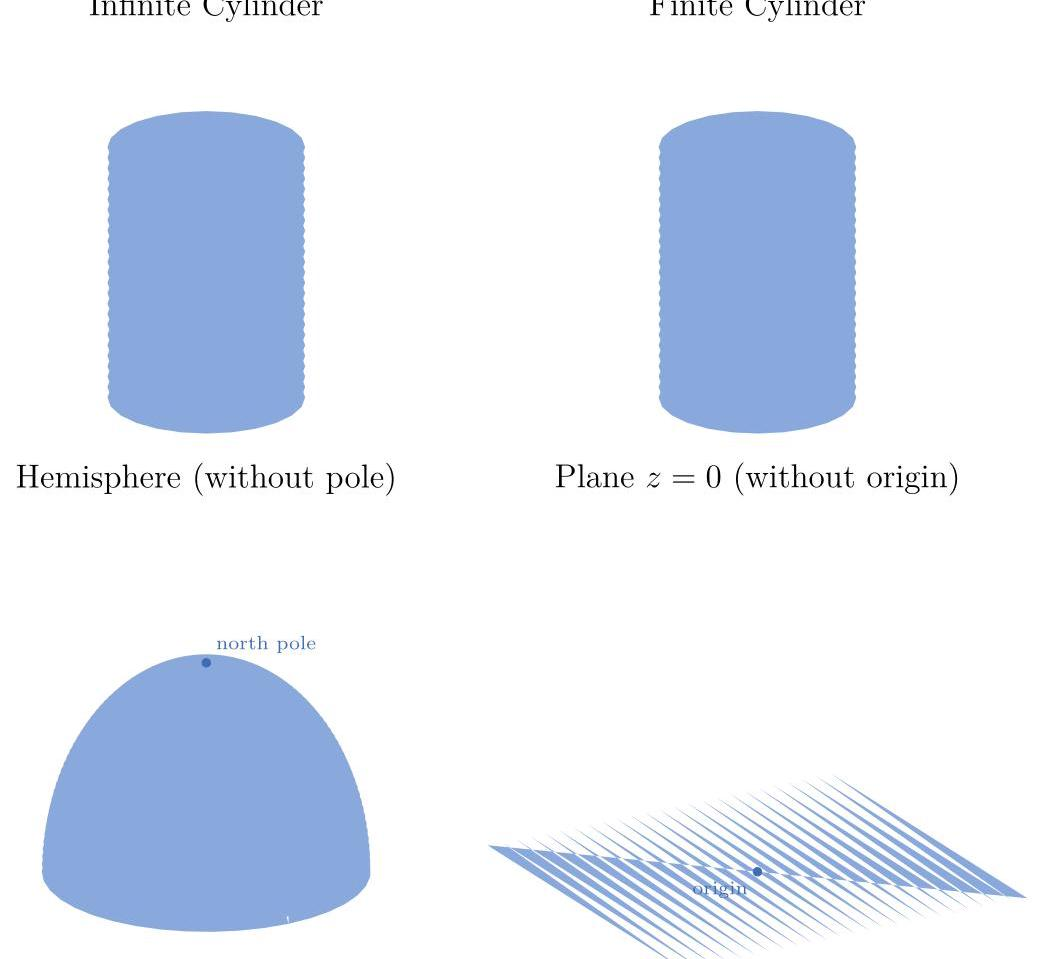
\includegraphics[max width=0.8\textwidth]{images/bo_d5bk0fbef24c73bipo90_10_272_241_1043_959_0.jpg}
\end{center}
\hspace*{3em} 

Finite Cylinder

A simpler version: take the intersection of the plane \(z = a\) with the infinite cylinder. It is clear that the intersection is a circle. We identify this circle with a circle of radius \({e}^{a}\) in the plane \(z = 0\) .

\begin{problem}[title=PROBLEM 3 (6 POINTS)]
For each map \(\Phi  : {\mathbb{R}}^{2} \rightarrow  {\mathbb{R}}^{3}\) , compute \({\Phi }_{x},{\Phi }_{y}\) and determine where \(\Phi\) is regular.

1. \(\Phi \left( {x,y}\right)  = \left( {{x}^{2},{y}^{2},{x}^{4}y}\right)\)

2. \(\Phi \left( {x,y}\right)  = \frac{1}{1 + {x}^{2} + {y}^{2}}\left( {{2x},{2y}, - 1 + {x}^{2} + {y}^{2}}\right)\)

3. \(\Phi \left( {x,y}\right)  = \left( {\left( {a + r\cos x}\right) \cos y,\left( {a + r\cos x}\right) \sin y,r\sin x}\right)\)
\end{problem}

Solution. For maps \(\Phi  : {\mathbb{R}}^{2} \rightarrow  {\mathbb{R}}^{3}\) compute the tangent map and determine regularity.

(1) \(\Phi \left( {x,y}\right)  = \left( {{x}^{2},{y}^{2},{x}^{4}y}\right)\) .

Compute partial derivatives:

\[
{\Phi }_{x} = \left( {{2x},0,4{x}^{3}y}\right) ,\;{\Phi }_{y} = \left( {0,{2y},{x}^{4}}\right) .
\]

Thus the tangent map (Jacobian) at \(\left( {x,y}\right)\) is the \(3 \times  2\) matrix with these columns. The map is regular at \(\left( {x,y}\right)\) iff the two columns are linearly independent, equivalently iff their cross product is nonzero:

\[
{\Phi }_{x} \times  {\Phi }_{y} = \left( {-8{x}^{3}{y}^{2}, - 8{x}^{3},{4xy}}\right) .
\]

This vector vanishes exactly when \(x = 0\) . Therefore \(\Phi\) is regular on \(\{ \left( {x,y}\right)  : x \neq  0\}\) and singular along the \(y\) -axis \(x = 0\) (at \(x = 0\) the rank drops: if \(x = 0,y \neq  0\) rank \(= 1\) ; at \(\left( {0,0}\right)\) rank \(= 0\) ).

(2) \(\Phi \left( {x,y}\right)  = \frac{1}{1 + {x}^{2} + {y}^{2}}\left( {{2x},{2y}, - 1 + {x}^{2} + {y}^{2}}\right)\) .

Let \({r}^{2} = {x}^{2} + {y}^{2}\) and \(d = 1 + {r}^{2}\) . This is the inverse stereographic map from \({\mathbb{R}}^{2}\) to the unit sphere \({S}^{2}\) . Compute the partials (omitted long algebra here) or recall the standard fact: the inverse stereographic projection is a smooth immersion everywhere on \({\mathbb{R}}^{2}\) . In particular the two partial derivatives are linearly independent for every \(\left( {x,y}\right)\) . One can check directly that

\[
{\Phi }_{x} = \frac{1}{{d}^{2}}\left( {2 - 2{x}^{2} + 2{y}^{2}, - {4xy},{4x}}\right) ,\;{\Phi }_{y} = \frac{1}{{d}^{2}}\left( {-{4xy},2 - 2{y}^{2} + 2{x}^{2},{4y}}\right) .
\]

\[
\begin{Vmatrix}{{\Phi }_{x} \times  {\Phi }_{y}}\end{Vmatrix} = \frac{4}{{\left( 1 + {r}^{2}\right) }^{2}} > 0\;\text{ for all }\left( {x,y}\right) ,
\]

hence \(\Phi\) is regular on all of \({\mathbb{R}}^{2}\) .

(3) \(\Phi \left( {x,y}\right)  = \left( {\left( {a + r\cos x}\right) \cos y,\left( {a + r\cos x}\right) \sin y,r\sin x}\right)\) , constants \(a,r \in  \mathbb{R}\) .

This is the standard torus parametrization (if \(a > 0,r > 0\) ). Compute partials:

\[
{\Phi }_{x} = \left( {-r\sin x\cos y, - r\sin x\sin y,r\cos x}\right) ,\;{\Phi }_{y} = \left( {-\left( {a + r\cos x}\right) \sin y,\left( {a + r\cos x}\right) \cos y,0}\right) .
\]

Their cross product equals

\[
{\Phi }_{x} \times  {\Phi }_{y} =  - r\left( {a + r\cos x}\right) \left( {\cos y,\cos x\sin y,\sin x}\right) ,
\]

so its magnitude is \(\left| {r\left( {a + r\cos x}\right) }\right|\) . Therefore the map is regular precisely where

\[
r\left( {a + r\cos x}\right)  \neq  0.
\]

In particular if \(r = 0\) the surface degenerates; if \(a > \left| r\right|\) then \(a + r\cos x > 0\) for all \(x\) and the parametrization is regular everywhere. If \(\left| a\right|  < \left| r\right|\) there are values of \(x\) with \(a + r\cos x = 0\) where the parametrization fails to be regular.

\section*{3.2 Exam-Qualifying Problems}

PROBLEM 4 (4 POINTS)

Let

\[
c\left( t\right)  = \left\{  \begin{array}{ll} \left( {t,{e}^{-1/{t}^{2}},0}\right) , & t > 0, \\  \left( {0,0,0}\right) , & t = 0, \\  \left( {t,0,{e}^{-1/{t}^{2}}}\right) , & t < 0. \end{array}\right.
\]

Sketch the curve and compute curvature and torsion; discuss the behavior of the \(T - N\) plane at \(t = 0\) .

Solution. Sketch and qualitative description. For \(t > 0\) the curve lies in the \(x - y\) plane and is the graph of \(y = {e}^{-1/{t}^{2}}\) , which is a smooth function tending to 0 faster than any power of \(t\) as \(t \downarrow  0\) . For \(t < 0\) the curve lies in the \(x - z\) plane as \(z = {e}^{-1/{t}^{2}}\) . At \(t = 0\) the curve passes through the origin. So the picture: near the origin both branches approach the \(x\) -axis tangentially, one branch "kicks" slightly in the \(y\) -direction for \(t > 0\) and the other branch "kicks" in the \(z\) -direction for \(t < 0\) . See sketch: a curve approaching the \(x\) -axis from two orthogonal off-axis directions.

\begin{center}
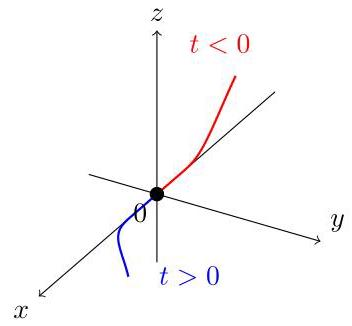
\includegraphics[max width=0.3\textwidth]{images/bo_d5bk0fbef24c73bipo90_11_195_1664_352_326_0.jpg}
\end{center}
\hspace*{3em} 

Derivatives and tangents. For \(t \neq  0\) compute

\[
\dot{c}\left( t\right)  = \left\{  \begin{array}{ll} \left( {1,\frac{2}{{t}^{3}}{e}^{-1/{t}^{2}},0}\right) , & t > 0, \\  \left( {1,0, - \frac{2}{{t}^{3}}{e}^{-1/{t}^{2}}}\right) , & t < 0. \end{array}\right.
\]

As \(t \rightarrow  {0}^{ \pm  }\) the exponential factors decay to 0 faster than any power, so \(\dot{c}\left( t\right)  \rightarrow  \left( {1,0,0}\right)\) . Thus the unit tangent \(T\left( t\right)  \rightarrow  \left( {1,0,0}\right)\) from both sides.

Curvature and torsion for \(t \neq  0\) . For \(t > 0\) the curve is planar in the \({xy}\) -plane, hence torsion \(\tau \left( t\right)  = 0\) for \(t > 0\) . Similarly \(\tau \left( t\right)  = 0\) for \(t < 0\) because that branch is planar in the \({xz}\) -plane. Thus \(\tau \left( t\right)  \equiv  0\) for all \(t \neq  0\) .

The curvature for \(t > 0\) is

\[
\kappa \left( t\right)  = \frac{\left| \dot{c} \times  \ddot{c}\right| }{{\left| \dot{c}\right| }^{3}} = 2{e}^{-\frac{1}{{t}^{2}}}\frac{\left| 3{t}^{2} - 2\right| }{{t}^{6}}.
\]

Because the non- \(x\) components (the small exponential terms and their derivatives) decay faster than any power of \(t\) as \(t \rightarrow  0\) , one checks that \(\kappa \left( t\right)  \rightarrow  0\) as \(t \rightarrow  {0}^{ \pm  }\) . Concretely: \(\dot{c} = \left( {1,\epsilon \left( t\right) ,0}\right) ,\ddot{c} = \left( {0,{\epsilon }_{1}\left( t\right) ,0}\right)\) with \(\epsilon ,{\epsilon }_{1} \rightarrow  0\) super-fast, so \(\dot{c} \times  \ddot{c}\) is of order \({\epsilon }_{1}\) and \({\left| \dot{c}\right| }^{3} \approx  1\) . Hence \(\kappa \left( t\right)  \rightarrow  0\) .

We may therefore conclude that curvature \(\kappa \left( t\right)  \rightarrow  0\) and torsion \(\tau \left( t\right)  = 0\) for \(t \rightarrow  {0}^{ \pm  }\) .

Behavior of the \(T - N\) plane at \(t = 0\) . The unit tangent \(T\left( t\right)\) tends to \(\left( {1,0,0}\right)\) from both sides. However the principal normal \(N\left( t\right)\) approaches different directions from the two sides: for \(t \downarrow  0\) (positive) the curve bends into the \(+ y\) -direction so \(N\left( t\right)  \rightarrow  \left( {0,1,0}\right)\) ; for \(t \uparrow  0\) (negative) the curve bends into the \(+ z\) -direction so \(N\left( t\right)  \rightarrow  \left( {0,0,1}\right)\) . Thus the limiting normal is not unique: the \(T - N\) plane for \(t > 0\) tends to the \(x - y\) plane, while for \(t < 0\) it tends to the \(x - z\) plane. At \(t = 0\) there is a continuous tangent but a discontinuous normal -the osculating plane jumps. This demonstrates that smoothness of the curve does not force continuity of the normal direction at points where higher derivatives vanish extremely fast.

\begin{problem}[title=PROBLEM 5 (6 POINTS)]
A generalized cone is the union of all lines through a point \(p\) and a regular space curve \(c\left( s\right)\) .

1. Sketch the construction.

2. Give a parametrization and determine where it is regular.

3. Show the same surface is obtained by replacing \(c\left( s\right)\) by its projection to the unit sphere centered at \(p\) .
\end{problem}

\section*{Solution. (1) Sketch.}

Sketch: take a point \(p\) and a space curve \(c\left( s\right)\) . For each \(s\) draw the straight line through \(p\) and \(c\left( s\right)\) . The union of all these lines is the generalized cone.

\section*{(2) Parametrization and regularity.}

A convenient parametrization is

\[
X\left( {s,t}\right)  = \left( {1 - t}\right) p + {tc}\left( s\right) ,\;\left( {s,t}\right)  \in  I \times  \left( {0,\infty }\right) ,
\]

where \(I\) is the parameter interval of the regular curve \(c\) . For each fixed \(s,t \mapsto  X\left( {s,t}\right)\) parametrizes the line through \(p\) and \(c\left( s\right)\) ; the whole surface is obtained by letting \(s\) vary.

Compute partial derivatives:

\[
{X}_{s}\left( {s,t}\right)  = t{c}^{\prime }\left( s\right) ,\;{X}_{t}\left( {s,t}\right)  = c\left( s\right)  - p.
\]

Their cross product is

\[
{X}_{s} \times  {X}_{t} = t\left( {{c}^{\prime }\left( s\right)  \times  \left( {c\left( s\right)  - p}\right) }\right) .
\]

Thus \(X\) is an immersion (i.e. a parametrized surface) precisely where

\[
t \neq  0\;\text{ and }\;{c}^{\prime }\left( s\right)  \times  \left( {c\left( s\right)  - p}\right)  \neq  0.
\]

So the cone is regular away from the apex \(\left( {t = 0\text{ corresponds to the apex }p}\right)\) and away from points \(s\) where the tangent vector \({c}^{\prime }\left( s\right)\) is parallel to the radius vector \(c\left( s\right)  - p\) (i.e. where the ruling line is tangent to the base curve).

(3) Replace \(c\) by a spherical curve.

Write \(r\left( s\right)  = c\left( s\right)  - p\) . For each \(s\) the line through \(p\) and \(c\left( s\right)\) equals the line \(\{ p + {\lambda r}\left( s\right)  : \lambda  \in  \mathbb{R}\}\) . Let \(\widetilde{c}\left( s\right)  = \frac{r\left( s\right) }{\parallel r\left( s\right) \parallel }\) be the unit vector pointing from \(p\) to \(c\left( s\right)\) . Then the same cone is obtained by the family of lines \(\{ p + \lambda \widetilde{c}\left( s\right)  : \lambda  \in  \mathbb{R}\}\) (indeed \(r\left( s\right)\) and \(\widetilde{c}\left( s\right)\) determine the same line). Thus one can replace \(c\) by \(\widetilde{c}\) , which lies on the unit sphere centered at \(p\) , and obtain the identical cone.

This completes Problem 5.

\section*{4 Homework 4}

\section*{4.1 Grade-Influencing Problems}

PROBLEM 1 (4 POINTS)

Show in two different ways that the set

\[
S = \left\{  {\left( {x,y,z}\right)  \in  {\mathbb{R}}^{3} : x{e}^{xy} - z = 0}\right\}
\]

is a surface. Find the tangent plane at \(\left( {2,0,2}\right)\) .

Solution. Method 1:

Let

\[
F\left( {x,y,z}\right)  = x{e}^{xy} - z.
\]

Then \(S = {F}^{-1}\left( 0\right)\) . Compute the gradient:

\[
\nabla F = \left( {{e}^{xy} + {xy}{e}^{xy},{x}^{2}{e}^{xy}, - 1}\right) .
\]

The third component is -1, hence \(\nabla F \neq  0\) everywhere. Therefore,0 is a regular value of \(F\) and \(S\) is a smooth surface by the regular value theorem.

Method 2:

\[
S = \left\{  {\left( {x,y,x{e}^{xy}}\right)  : \left( {x,y}\right)  \in  {\mathbb{R}}^{2}}\right\}
\]

is the graph of some smooth function. Thus \(S\) is a surface.

Tangent plane at \(\left( {2,0,2}\right)\) . The tangent plane to \(F\left( {x,y,z}\right)  = 0\) at \(\left( {2,0,2}\right)\) satisfies

\[
\nabla F\left( {2,0,2}\right)  \cdot  \left( {\left( {x,y,z}\right)  - \left( {2,0,2}\right) }\right)  = 0.
\]

Compute \(\nabla F\left( {2,0,2}\right)  = \left( {1,4, - 1}\right)\) , so

\[
\left( {x - 2}\right)  + {4y} - \left( {z - 2}\right)  = 0\; \Rightarrow  \;x + {4y} - z = 0.
\]

PROBLEM 2 (5 POINTS)

1. Show that

\[
C = \left\{  {\left( {x,y,z}\right)  \in  {\mathbb{R}}^{3} : {x}^{2} + {y}^{2} + {z}^{4} = 1}\right\}
\]

is a surface.

2. Construct a smooth bijection

\[
\varphi  : {\mathbb{R}}^{3} \smallsetminus  \{ 0\}  \rightarrow  {\mathbb{R}}^{3} \smallsetminus  \{ 0\}
\]

with smooth inverse such that \(\varphi\) maps \(C\) bijectively onto the unit sphere \({S}^{2}\) .

(1) Regular value test. Let

\[
F\left( {x,y,z}\right)  = {x}^{2} + {y}^{2} + {z}^{4} - 1,\;\nabla F = \left( {{2x},{2y},4{z}^{3}}\right) .
\]

The gradient vanishes only at \(\left( {0,0,0}\right)\) , which does not belong to \(C\) . Hence 0 is a regular value, and \(C\) is a smooth surface.

(2) Constructing a smooth bijection. There are many different diffeomorphisms. We write the simplest one: Consider the equation

\[
{x}^{2} + {y}^{2} + {z}^{4} = 1
\]

We can transform it into

\[
\frac{{x}^{2}}{1 + {z}^{2}} + \frac{{y}^{2}}{1 + {z}^{2}} + {z}^{2} = 1
\]

Thus, we may define \(\varphi\) to be

\[
\left( {x,y,z}\right)  \mapsto  \left( {\frac{x}{\sqrt{z + {z}^{2}}},\frac{y}{\sqrt{1 + {z}^{2}}},z}\right) .
\]

The geometric intuition behind this is that we only stretch in the xy-direction, slimming this 'chubby' sphere into a standard sphere.

\begin{problem}[title=PROBLEM 3 (5 POINTS)]
The Minkowski inner product on \({\mathbb{R}}^{3}\) is

\[
\langle v,w\rangle  = {v}_{1}{w}_{1} + {v}_{2}{w}_{2} - {v}_{3}{w}_{3}.
\]

For which \(c \in  \mathbb{R}\) is

\[
C = \left\{  {v \in  {\mathbb{R}}^{3} : \langle v,v\rangle  = c}\right\}
\]

a surface? What type of surface is it? Find the tangent space \({T}_{v}C\) when it is a surface.
\end{problem}

Solution. Solution. Let us first explain this inner product. In Euclidean space, we are used to the distance formula:

\[
d{s}^{2} = d{x}^{2} + d{y}^{2} + d{z}^{2}
\]

This is a positive-definite metric, meaning any nonzero displacement has a positive length.

In relativity, we deal with spacetime, represented as a 4-vector \(\left( {t,x,y,z}\right)\) . Here, the "distance" between events is called the interval, which combines space and time.

The Minkowski metric in four-dimensional spacetime is usually written as:

\[
d{s}^{2} =  - {c}^{2}d{t}^{2} + d{x}^{2} + d{y}^{2} + d{z}^{2}
\]

or sometimes as

\[
d{s}^{2} = {c}^{2}d{t}^{2} - d{x}^{2} - d{y}^{2} - d{z}^{2}
\]

\begin{itemize}\relax
\item\relax \(c\) is the speed of light (often set to 1 in natural units).
\end{itemize}

\begin{itemize}\relax
\item\relax The minus sign for the time component is essential - it distinguishes time from space.
\end{itemize}

\begin{itemize}\relax
\item\relax Timelike intervals \(\left( {d{s}^{2} < 0}\right.\) in the first convention): events can be causally connected (something can travel from one to the other slower than light).
\end{itemize}

\begin{itemize}\relax
\item\relax Spacelike intervals \(\left( {d{s}^{2} > 0}\right)\) : events cannot influence each other; they are separated in space.
\end{itemize}

\begin{itemize}\relax
\item\relax Lightlike or null intervals \(\left( {d{s}^{2} = 0}\right)\) : events connected by light.
\end{itemize}

So the Minkowski metric encodes the causal structure of spacetime. Let

\[
F\left( {x,y,z}\right)  = {x}^{2} + {y}^{2} - {z}^{2} - c,\;\nabla F = \left( {{2x},{2y}, - {2z}}\right) .
\]

The gradient vanishes only at the origin. If \(c \neq  0\) , the origin is not on \(C\) , so \(C\) is a smooth surface. If \(c = 0\) , the origin belongs to \(C\) , and the gradient vanishes there - hence not smooth (a cone).

Classification.

\begin{itemize}\relax
\item\relax \(c > 0\) : one-sheeted hyperboloid.
\end{itemize}

\begin{itemize}\relax
\item\relax \(c < 0\) : two-sheeted hyperboloid.
\end{itemize}

\begin{itemize}\relax
\item\relax \(c = 0\) : double cone (not smooth at the vertex).
\end{itemize}

Tangent space. For \(v = \left( {x,y,z}\right)  \in  C\) (with \(c \neq  0\) ),

\[
{T}_{v}C = \left\{  {w \in  {\mathbb{R}}^{3} : \nabla F\left( v\right)  \cdot  w = 0}\right\}   = \left\{  {w : {2x}{w}_{1} + {2y}{w}_{2} - {2z}{w}_{3} = 0}\right\}  .
\]

Equivalently,

\[
{T}_{v}C = \left\{  {w : \langle v,w{\rangle }_{\text{ Mink }} = 0}\right\}  .
\]

Thus the tangent space consists of all Minkowski-orthogonal vectors to \(v\) .

\begin{problem}[title=PROBLEM 4 (4 POINTS)]
Show that

\[
\left\{  {\left( {x,y,z}\right)  \in  {\mathbb{R}}^{3} : {\left( {x}^{2} + {y}^{2} + {z}^{2} + {R}^{2} - {r}^{2}\right) }^{2} = 4{R}^{2}\left( {{x}^{2} + {y}^{2}}\right) }\right\}
\]

is a surface for \(0 < r < R\) .
\end{problem}

Solution. Consider the surface

\[
{\left( {x}^{2} + {y}^{2} + {z}^{2} + {R}^{2} - {r}^{2}\right) }^{2} = 4{R}^{2}\left( {{x}^{2} + {y}^{2}}\right) .
\]

Let

\[
x = \rho \cos \phi ,\;y = \rho \sin \phi ,\;\rho  = \sqrt{{x}^{2} + {y}^{2}}.
\]

The equation becomes

\[
{\left( {\rho }^{2} + {z}^{2} + {R}^{2} - {r}^{2}\right) }^{2} = 4{R}^{2}{\rho }^{2}.
\]

Taking the positive square root gives

\[
{\rho }^{2} + {z}^{2} + {R}^{2} - {r}^{2} = {2R\rho }
\]

which can be rearranged as

\[
{z}^{2} + {\left( \rho  - R\right) }^{2} = {r}^{2}.
\]

The equation \({z}^{2} + {\left( \rho  - R\right) }^{2} = {r}^{2}\) represents a circle of radius \(r\) in the \({\rho z}\) -plane, centered at \(\left( {\rho  = R,z = 0}\right)\) . Together, these constraints describe a small circle of radius \(r\) revolving around a large circle of radius \(R\) , producing the torus.

Let

\[
F\left( {x,y,z}\right)  = {\left( {x}^{2} + {y}^{2} + {z}^{2} + {R}^{2} - {r}^{2}\right) }^{2} - 4{R}^{2}\left( {{x}^{2} + {y}^{2}}\right) .
\]

We show \(\nabla F \neq  0\) on \({F}^{-1}\left( 0\right)\) . Let \(S = {x}^{2} + {y}^{2} + {z}^{2} + {R}^{2} - {r}^{2}\) . Then

\[
\nabla F = \left( {{4x}\left( {S - 2{R}^{2}}\right) ,{4y}\left( {S - 2{R}^{2}}\right) ,{4zS}}\right) .
\]

If \(\nabla F = 0\) , then either \(x = y = 0\) or \(S = 2{R}^{2}\) .

If \(S = 2{R}^{2}\) , then \({x}^{2} + {y}^{2} + {z}^{2} = {R}^{2} + {r}^{2}\) , and from \(F = 0\) we get \({x}^{2} + {y}^{2} = {R}^{2}\) , hence \({z}^{2} = {r}^{2}\) . At those points \(\partial F/\partial z = {4zS} = 8{R}^{2}z \neq  0\) (since \(z =  \pm  r \neq  0\) ). If \(x = y = 0\) , then \(S = 0\) would imply \({z}^{2} = {r}^{2} - {R}^{2} < 0\) , impossible. Hence \(\nabla F \neq  0\) . Therefore \({F}^{-1}\left( 0\right)\) is a smooth surface - the standard torus.

\section*{4.2 Exam-Qualifying Problems}

PROBLEM 5 (6 POINTS)

Show that

\[
P = \left\{  {\left( {x,y,z}\right)  \in  {\mathbb{R}}^{3} : z\left( {{x}^{2} + {y}^{2}}\right)  = {2xy},\left( {x,y}\right)  \neq  \left( {0,0}\right) }\right\}
\]

is a surface, called the Plücker's conoid. Show that it is a ruled surface.

Solution. The equation gives

\[
z = \frac{2xy}{{x}^{2} + {y}^{2}},\;\left( {x,y}\right)  \neq  \left( {0,0}\right) ,
\]

so \(P\) is the graph of a smooth function, thus a smooth surface.

Use polar coordinates \(x = r\cos \theta ,y = r\sin \theta ,r > 0\) . Then

\[
z = \sin \left( {2\theta }\right) ,
\]

and a parametrization is

\[
\sigma \left( {r,\theta }\right)  = \left( {r\cos \theta ,r\sin \theta ,\sin \left( {2\theta }\right) }\right) .
\]

Compute

\[
{\sigma }_{r} = \left( {\cos \theta ,\sin \theta ,0}\right) ,\;{\sigma }_{\theta } = \left( {-r\sin \theta ,r\cos \theta ,2\cos \left( {2\theta }\right) }\right) .
\]

Their cross product is

\[
{\sigma }_{r} \times  {\sigma }_{\theta } = \left( {2\cos \left( {2\theta }\right) \sin \theta , - 2\cos \left( {2\theta }\right) \cos \theta ,r}\right) ,
\]

whose norm is \(\sqrt{4{\cos }^{2}\left( {2\theta }\right)  + {r}^{2}} > 0\) for \(r > 0\) , hence \(\sigma\) is an immersion and \(P\) a smooth surface.

For fixed \(\theta  = {\theta }_{0}\) , the set

\[
\left\{  {\left( {r\cos {\theta }_{0},r\sin {\theta }_{0},\sin \left( {2{\theta }_{0}}\right) }\right)  : r > 0}\right\}
\]

is a straight line. Thus \(P\) is a ruled surface formed by a family of straight lines.

For a better reference, see Plücker's conoid on Wikipedia

\begin{problem}[title=PROBLEM 6 (6 POINTS)]
Let \(\chi  : {S}^{2} \smallsetminus  \{ N\}  \rightarrow  {\mathbb{R}}^{2}\) be the stereographic projection from the north pole:

\[
\chi \left( {x,y,z}\right)  = \left( {\frac{x}{1 - z},\frac{y}{1 - z}}\right) .
\]

1. Find its inverse \(\Phi  = {\chi }^{-1}\) and show that it is a chart for \({S}^{2}\) .

2. Compute \(\partial \Phi /\partial u\) and \(\partial \Phi /\partial v\) at \(\left( {u,v}\right)  \in  {\mathbb{R}}^{2}\) .

(1) Inverse map. The standard inverse of stereographic projection is

\[
\Phi \left( {u,v}\right)  = \left( {\frac{2u}{1 + {u}^{2} + {v}^{2}},\frac{2v}{1 + {u}^{2} + {v}^{2}},\frac{{u}^{2} + {v}^{2} - 1}{1 + {u}^{2} + {v}^{2}}}\right) .
\]

This map is smooth and bijective onto \({S}^{2} \smallsetminus  \{ N\}\) , hence a valid coordinate chart.

(2) Partial derivatives. Let \(D = 1 + {u}^{2} + {v}^{2}\) . Then

\[
\Phi \left( {u,v}\right)  = \left( {\frac{2u}{D},\frac{2v}{D},\frac{{u}^{2} + {v}^{2} - 1}{D}}\right) .
\]

Compute

\[
\frac{\partial \Phi }{\partial u} = \frac{2}{{D}^{2}}\left( {1 - {u}^{2} + {v}^{2}, - {2uv},{2u}}\right) ,
\]

\[
\frac{\partial \Phi }{\partial v} = \frac{2}{{D}^{2}}\left( {-{2uv},1 + {u}^{2} - {v}^{2},{2v}}\right) .
\]

These vectors lie in \({T}_{\Phi \left( {u,v}\right) }{S}^{2}\) and are linearly independent.
\end{problem}

\section*{5 Homework 5}

\section*{5.1 Grade-Influencing Problems}

PROBLEM 1 (5 POINTS)

Define the vector fields

\[
X = {\partial }_{x},\;Y = {\partial }_{y},\;E = x{\partial }_{x} + y{\partial }_{y}
\]

on \({\mathbb{R}}^{2}\) (the plane \(z = 0\) ). Consider polar coordinates

\[
\Phi  : \left( {r,\varphi }\right)  \mapsto  \left( {x,y}\right)  = \left( {r\cos \varphi ,r\sin \varphi }\right) ,\;r > 0,\varphi  \in  \left( {0,{2\pi }}\right) .
\]

Compute the representations of \(X,Y,E\) in the chart \(\Phi\) , i.e. write them in terms of \({\partial }_{r}\) and \({\partial }_{\varphi }\) .

Solution. Solution. Use the change-of-coordinates formulas. We have

\[
x = r\cos \varphi
\]

\[
{\partial }_{r} = \cos \varphi {\partial }_{x} + \sin \varphi {\partial }_{y},
\]

\[
{\partial }_{\varphi } =  - r\sin \varphi {\partial }_{x} + r\cos \varphi {\partial }_{y}.
\]

\[
y = r\sin \varphi ,
\]

Solve for \({\partial }_{x},{\partial }_{y}\) in terms of \({\partial }_{r},{\partial }_{\varphi }\) . Treat the linear system

\[
\left( \begin{matrix} {\partial }_{r} \\  {\partial }_{\varphi }/r \end{matrix}\right)  = \left( \begin{matrix} \cos \varphi & \sin \varphi \\   - \sin \varphi & \cos \varphi  \end{matrix}\right) \left( \begin{array}{l} {\partial }_{x} \\  {\partial }_{y} \end{array}\right) .
\]

The matrix on the right is orthogonal, so its inverse is its transpose. Thus

\[
{\partial }_{x} = \cos \varphi {\partial }_{r} - \frac{\sin \varphi }{r}{\partial }_{\varphi },
\]

\[
{\partial }_{y} = \sin \varphi {\partial }_{r} + \frac{\cos \varphi }{r}{\partial }_{\varphi }.
\]

Therefore

\[
X = {\partial }_{x} = \cos \varphi {\partial }_{r} - \frac{\sin \varphi }{r}{\partial }_{\varphi }
\]

\[
Y = {\partial }_{y} = \sin \varphi {\partial }_{r} + \frac{\cos \varphi }{r}{\partial }_{\varphi },
\]

\[
E = x{\partial }_{x} + y{\partial }_{y} = r{\partial }_{r}.
\]

(Notice \(E\) simplifies because \(x{\partial }_{x} + y{\partial }_{y} = r\left( {\cos \varphi {\partial }_{x} + \sin \varphi {\partial }_{y}}\right)  = r{\partial }_{r}\) .)

Remark: here, \(E\) is called the Euler vector field. We use it to define homogeneous functions. Let \(f : {\mathbb{R}}^{n} \rightarrow  \mathbb{R}\) be a homogeneous smooth function of degree \(d\) , i.e.

\[
\exists d \in  \mathbb{R},f\left( {\lambda x}\right)  = {\lambda }^{d}f\left( x\right) ,\;\forall \lambda  > 0,x \in  {\mathbb{R}}^{n} \smallsetminus  \{ 0\} .
\]

We can show that \(E\left( f\right)  = {cf}\) .

\begin{problem}[title=PROBLEM 2 (8 POINTS)]
The torus \(\mathbb{T}\) with major radius \(R\) and minor radius \(r\) is defined by

\[
\mathbb{T} = \left\{  {\left( {x,y,z}\right)  \in  {\mathbb{R}}^{3} : {\left( \sqrt{{x}^{2} + {y}^{2}} - R\right) }^{2} + {z}^{2} = {r}^{2}}\right\}  .
\]

We consider the chart \(\Phi  : \left( {0,{2\pi }}\right)  \times  \left( {0,{2\pi }}\right)  \rightarrow  {\mathbb{R}}^{3}\) on \(\mathbb{T}\) defined by

\[
\Phi \left( {\theta ,\varphi }\right)  = \left( {\left( {R + r\cos \varphi }\right) \cos \theta ,\left( {R + r\cos \varphi }\right) \sin \theta ,r\sin \varphi }\right) .
\]

1. When is a vector \(v \in  {\mathbb{R}}^{3}\) tangent to \(\mathbb{T}\) at a point \(\left( {x,y,z}\right)  \in  \mathbb{T}\) ?

2. Compute the derivative \({T}_{p}\Phi  : {\mathbb{R}}^{2} \rightarrow  {T}_{\Phi \left( p\right) }\mathbb{T}\) at a point \(p = \left( {\theta ,\varphi }\right)\) .

3. On the chart domain, we have canonical basis vector fields \({\partial }_{\theta }\) and \({\partial }_{\varphi }\) . Compute the induced vector fields \({\partial }_{\theta }^{\Phi }\) and \({\partial }_{\varphi }^{\Phi }\) on \(\mathbb{T}\) . Since \(\mathbb{T} \subset  {\mathbb{R}}^{3}\) , express these induced vector fields in terms of the canonical basis \({\partial }_{x},{\partial }_{y},{\partial }_{z}\) on \({\mathbb{R}}^{3}\) . Show that

\[
{\partial }_{\theta }^{\Phi } =  - y{\partial }_{x} + x{\partial }_{y},\;\left( {x,y,z}\right)  \in  \mathbb{T},
\]

and find a similar expression for \({\partial }_{\varphi }^{\Phi }\) .

4. Visualize these induced vector fields on the torus \(\mathbb{T}\) .
\end{problem}

Solution. 1. A vector \(v \in  {\mathbb{R}}^{3}\) is tangent to \(\mathbb{T}\) at a point \(p = \left( {x,y,z}\right)  \in  \mathbb{T}\) precisely when it is orthogonal to a normal vector of the surface at \(p\) . Equivalently, if \(F\left( {x,y,z}\right)  = {\left( \sqrt{{x}^{2} + {y}^{2}} - R\right) }^{2} + {z}^{2} - {r}^{2}\) , then

\[
v \in  {T}_{p}\mathbb{T} \Leftrightarrow  v \cdot  \nabla F\left( p\right)  = 0.
\]

In the parametrized chart one usually use the two coordinate tangent vectors \({\partial }_{\theta }\Phi\) and \({\partial }_{\varphi }\Phi\) which span the tangent plane.

2. Compute the partial derivatives of \(\Phi\) :

\[
{\Phi }_{\theta }\left( {\theta ,\varphi }\right)  = {\partial }_{\theta }\Phi  = \left( {-\left( {R + r\cos \varphi }\right) \sin \theta ,\left( {R + r\cos \varphi }\right) \cos \theta ,0}\right) ,
\]

\[
{\Phi }_{\varphi }\left( {\theta ,\varphi }\right)  = {\partial }_{\varphi }\Phi  = \left( {-r\sin \varphi \cos \theta , - r\sin \varphi \sin \theta ,r\cos \varphi }\right) .
\]

Therefore the differential \({T}_{p}\Phi  : {\mathbb{R}}^{2} \rightarrow  {T}_{\Phi \left( p\right) }\mathbb{T}\) maps the coordinate basis vectors to these two vectors.

3. We can rewrite the first induced vector field in ambient coordinates using the fact that

\[
x = \left( {R + r\cos \varphi }\right) \cos \theta ,\;y = \left( {R + r\cos \varphi }\right) \sin \theta .
\]

Hence

\[
{\Phi }_{\theta } = \left( {-\left( {R + r\cos \varphi }\right) \sin \theta }\right) {\partial }_{x} + \left( {\left( {R + r\cos \varphi }\right) \cos \theta }\right) {\partial }_{y} + 0{\partial }_{z}
\]

\[
=  - y{\partial }_{x} + x{\partial }_{y}.
\]

This establishes the required identity

\[
{\partial }_{\Phi ,\theta } =  - y{\partial }_{x} + x{\partial }_{y}\;\text{ on }\mathbb{T}.
\]

For \({\Phi }_{\varphi }\) we express it in terms of \(x,y,z\) as follows. Let \(\rho  \mathrel{\text{ := }} \sqrt{{x}^{2} + {y}^{2}} = R + r\cos \varphi\) . Then \(z = r\sin \varphi\) and \(r\cos \varphi  = \rho  - R\) . Thus

\[
{\Phi }_{\varphi } = \left( {-r\sin \varphi \cos \theta , - r\sin \varphi \sin \theta ,r\cos \varphi }\right)
\]

\[
=  - \frac{z}{\rho }\left( {x{\partial }_{x} + y{\partial }_{y}}\right)  + \left( {\rho  - R}\right) {\partial }_{z}.
\]

So an equivalent ambient expression is

\[
{\partial }_{\Phi ,\varphi } =  - \frac{z}{\sqrt{{x}^{2} + {y}^{2}}}\left( {x{\partial }_{x} + y{\partial }_{y}}\right)  + \left( {\sqrt{{x}^{2} + {y}^{2}} - R}\right) {\partial }_{z}
\]

(One may check this formula is algebraically identical to the component form above.)

4. Visualization: \({\partial }_{\Phi ,\theta }\) is the vector field that goes once around the central circle (the \(\theta\) -direction): at each point it is tangent to the circle lying in the horizontal plane through the point, and equals the generator of rotation about the \(z\) -axis restricted to the torus. The field \({\partial }_{\Phi ,\varphi }\) runs along the small circular cross-sections (the meridional circles) of the torus. Together they provide the standard torus frame (longitudinal and meridional directions).

\begin{problem}[title=PROBLEM 3 (4 POINTS)]
Consider the path \(c : \left\lbrack  {0,\frac{1}{2}\pi }\right\rbrack   \rightarrow  {\mathbb{R}}^{2}\) given by

\[
c\left( t\right)  = \left( {a\cos t,b\sin t}\right) ,\;a,b > 0.
\]

Let \(\alpha  = {xydx} + {x}^{2}{ydy}\) . Compute \({\int }_{c}\alpha\) .
\end{problem}

Solution. Parameterize and compute

\[
x\left( t\right)  = a\cos t,
\]

\[
{dx} =  - a\sin {tdt},
\]

\[
y\left( t\right)  = b\sin t,
\]

\[
{dy} = b\cos {tdt}.
\]

The pullback integrand is

\[
\alpha \left( {c\left( t\right) }\right) \left( {\dot{c}\left( t\right) }\right)  = {xydx}\left( \dot{c}\right)  + {x}^{2}{ydy}\left( \dot{c}\right)
\]

\[
= \left( {a\cos t}\right) \left( {b\sin t}\right) \left( {-a\sin t}\right)  + \left( {{a}^{2}{\cos }^{2}t}\right) \left( {b\sin t}\right) \left( {b\cos t}\right)
\]

\[
=  - {a}^{2}b\cos t{\sin }^{2}t + {a}^{2}{b}^{2}{\cos }^{3}t\sin t\text{ . }
\]

The total integral is

\[
{\int }_{0}^{\frac{1}{2}\pi }\left( {-{a}^{2}b\cos t{\sin }^{2}t + {a}^{2}{b}^{2}{\cos }^{3}t\sin t}\right) {dt} = 0.
\]

So \({\int }_{c}\alpha  =  - \frac{{a}^{2}b}{3} + \frac{{a}^{2}{b}^{2}}{4}\) for all positive \(a,b\) .

\begin{problem}[title=PROBLEM 4 (4 POINTS)]
Consider polar chart \(\Phi  : \left( {r,\theta }\right)  \mapsto  \left( {x,y}\right)  = \left( {r\cos \theta ,r\sin \theta }\right)\) on \(S = {\mathbb{R}}^{2} \smallsetminus  \{ 0\}\) . For the 1-forms on \(S\) below compute their chart representations \({\alpha }_{\Phi } = {\alpha }_{r}{dr} + {\alpha }_{\theta }{d\theta }\) .

1. \(\alpha  = {xdy} - {ydx}\) .

2. \(\alpha  = {xdy} + {ydx}\) .
\end{problem}

Solution. Use

\[
{dx} = \cos {\theta dr} - r\sin {\theta d\theta },\;{dy} = \sin {\theta dr} + r\cos {\theta d\theta }.
\]

(1) Compute

\[
{xdy} - {ydx} = \left( {r\cos \theta }\right) \left( {\sin {\theta dr} + r\cos {\theta d\theta }}\right)  - \left( {r\sin \theta }\right) \left( {\cos {\theta dr} - r\sin {\theta d\theta }}\right)
\]

\[
= r\left( {\cos \theta \sin \theta  - \sin \theta \cos \theta }\right) {dr} + {r}^{2}\left( {{\cos }^{2}\theta  + {\sin }^{2}\theta }\right) {d\theta }
\]

\[
= {r}^{2}{d\theta }\text{ . }
\]

Hence \({\alpha }_{r} = 0,{\alpha }_{\theta } = {r}^{2}\) .

(2) Similarly

\[
{xdy} + {ydx} = r\left( {\cos \theta \sin \theta  + \sin \theta \cos \theta }\right) {dr} + {r}^{2}\left( {{\cos }^{2}\theta  - {\sin }^{2}\theta }\right) {d\theta }
\]

\[
= {2r}\sin \theta \cos {\theta dr} + {r}^{2}\cos {2\theta d\theta }
\]

\[
= r\sin \left( {2\theta }\right) {dr} + {r}^{2}\cos \left( {2\theta }\right) {d\theta }.
\]

So \({\alpha }_{r} = r\sin \left( {2\theta }\right)\) and \({\alpha }_{\theta } = {r}^{2}\cos \left( {2\theta }\right)\) . (One may also note \({xdy} + {ydx} = d\left( {xy}\right)\) and express \({xy} = \frac{1}{2}{r}^{2}\sin {2\theta }\) .)

\section*{5.2 Exam-Qualifying Problems}

PROBLEM 5 (8 POINTS)

For each 1-form on \({\mathbb{R}}^{3}\) find a potential \(f\) with \(\alpha  = {df}\) .

1. \(\alpha  = {ydz} + {zdy}\) .

2. \(\alpha  = {xdx} + {y}^{2}{dy} + {z}^{3}{dz}\) .

3. \(\alpha  = 3{x}^{2}{y}^{2}{zdx} + 2{x}^{3}{yzdy} + {x}^{3}{y}^{2}{dz}\) .

Solution. We seek \(f\left( {x,y,z}\right)\) with \({\partial }_{x}f,{\partial }_{y}f,{\partial }_{z}f\) equal to the coefficients.

1. From \({\partial }_{x}f = 0,{\partial }_{y}f = z,{\partial }_{z}f = y\) . Integrate \({\partial }_{y}f = z\) to get \(f = {yz} + h\left( {x,z}\right)\) . Then \({\partial }_{z}f = y + {\partial }_{z}h\) must equal \(y\) , hence \({\partial }_{z}h = 0\) so \(h = h\left( x\right)\) . Finally \({\partial }_{x}f = {h}^{\prime }\left( x\right)  = 0\) so \(h\) is constant. Thus one potential is

\[
f\left( {x,y,z}\right)  = {yz} + C.
\]

2. Integrate componentwise:

\[
f\left( {x,y,z}\right)  = \frac{1}{2}{x}^{2} + \frac{1}{3}{y}^{3} + \frac{1}{4}{z}^{4} + C,
\]

which indeed yields \({df} = {xdx} + {y}^{2}{dy} + {z}^{3}{dz}\) .

3. Integrate \({\partial }_{x}f = 3{x}^{2}{y}^{2}z\) w.r.t. \(x\) to get \(f = {x}^{3}{y}^{2}z + g\left( {y,z}\right)\) . Then \({\partial }_{y}f = 2{x}^{3}{yz} + {\partial }_{y}g\) must equal \(2{x}^{3}{yz}\) , so \({\partial }_{y}g = 0\) and \(g = g\left( z\right)\) . Finally \({\partial }_{z}f = {x}^{3}{y}^{2} + {g}^{\prime }\left( z\right)\) must equal \({x}^{3}{y}^{2}\) , so \({g}^{\prime }\left( z\right)  = 0\) . Hence

\[
f\left( {x,y,z}\right)  = {x}^{3}{y}^{2}z + C.
\]

\begin{problem}[title=PROBLEM 6 (8 POINTS)]
For \(a \in  \mathbb{R}\) set on \({\mathbb{R}}^{3} \smallsetminus  \{ 0\}\)

\[
\alpha  = {\left( {x}^{2} + {y}^{2} + {z}^{2}\right) }^{a}\left( {{xdx} + {ydy} + {zdz}}\right) .
\]

Define for fixed nonzero \(x \in  {\mathbb{R}}^{3}\) the radial curve

\[
{c}_{x} : ( - \infty ,0\rbrack  \rightarrow  {\mathbb{R}}^{3},\;{c}_{x}\left( t\right)  = \left( {1 - t}\right) x.
\]

The problems are:

1. Sketch \({c}_{x}\) .

2. Determine for which \(a\) the function \(g\left( x\right)  = {\int }_{{c}_{x}}\alpha\) is well-defined for all \(x \neq  0\) , and compute \(g\left( x\right)\) .

3. For those \(a\) verify \({dg} = \alpha\) .

4. Relate the result to Newtonian gravitational potential.
\end{problem}

Solution. Along the radial path \({c}_{x}\left( t\right)  = {sx}\) with \(s = 1 - t \in  \lbrack 1,\infty )\) we have \({c}_{x}^{\prime }\left( t\right)  = x\) , and \({\begin{Vmatrix}{c}_{x}\left( t\right) \end{Vmatrix}}^{2} = {s}^{2}\parallel x{\parallel }^{2}\) . Evaluating the 1-form on the tangent gives

\[
\alpha \left( {{c}_{x}\left( t\right) }\right) \left( {{c}_{x}^{\prime }\left( t\right) }\right)  = {\left( {s}^{2}\parallel x{\parallel }^{2}\right) }^{a}\left( {\left( {sx}\right)  \cdot  x}\right)  = {s}^{2a}\parallel x{\parallel }^{2a} \cdot  s\parallel x{\parallel }^{2} = {s}^{{2a} + 1}\parallel x{\parallel }^{{2a} + 2}.
\]

Hence

\[
{\int }_{c}\alpha  = {\int }_{s = 1}^{\infty }{s}^{{2a} + 1}\parallel x{\parallel }^{{2a} + 2}{ds}.
\]

As a well-known fact, we have

\[
{\int }_{0}{s}^{{2a} + 1}{ds} < \infty  \Leftrightarrow  a <  - 1.
\]

Therefore the line integral defining

\[
g\left( x\right)  \mathrel{\text{ := }} {\int }_{{c}_{x}}\alpha
\]

is finite for \(a <  - 1\) and equals

\[
g\left( x\right)  = \frac{\parallel x{\parallel }^{{2a} + 2}}{{2a} + 2}. \tag{1}
\]

To verify \({dg} = \alpha\) for \(a <  - 1\) , compute

\[
{dg} = \frac{{2a} + 2}{{2a} + 2}\parallel x{\parallel }^{2a}\left( {{xdx} + {ydy} + {zdz}}\right)  = \parallel x{\parallel }^{2a}\left( {{xdx} + {ydy} + {zdz}}\right)  = \alpha ,
\]

which matches the definition of \(\alpha\) .

Recall that the Newtonian gravitational potential

\[
{E}_{P} =  - \frac{GMm}{r}.
\]

Take \(a =  - \frac{3}{2}.g\left( x\right)  =  - \frac{1}{r}\) is the Newtonian gravitational potential of some object with mess \(\frac{1}{GM}\) and position \(x\) .

\section*{6 Homework 6}

\section*{6.1 Grade-Influencing Problems}

PROBLEM 1 (5 POINTS)

Consider the forms on \({\mathbb{R}}^{3}\)

\[
\alpha  = {xdx} - {ydy},\;\beta  = {zdx} \land  {dy} + {xdy} \land  {dz},\;\gamma  = {zdy}.
\]

Calculate

1. \(\alpha  \land  \beta\) and \(\alpha  \land  \gamma\) ,

2. \({d\alpha },{d\beta }\) , and \({d\gamma }\) .

Solution. (1) Wedge products.

\[
\alpha  \land  \beta  = \left( {{xdx} - {ydy}}\right)  \land  \left( {{zdx} \land  {dy} + {xdy} \land  {dz}}\right) .
\]

All terms with a repeated \({dx}\) or \({dy}\) vanish, so the only nonzero contribution is

\[
\left( {xdx}\right)  \land  \left( {{xdy} \land  {dz}}\right)  = {x}^{2}{dx} \land  {dy} \land  {dz}.
\]

Hence

\[
\alpha  \land  \beta  = {x}^{2}{dx} \land  {dy} \land  {dz}
\]

Next

\[
\alpha  \land  \gamma  = \left( {{xdx} - {ydy}}\right)  \land  \left( {zdy}\right) .
\]

The \({dy} \land  {dy}\) term vanishes, leaving

\[
\left( {xdx}\right)  \land  \left( {zdy}\right)  = {xzdx} \land  {dy}.
\]

Thus

\[
\alpha  \land  \gamma  = {xzdx} \land  {dy}.
\]

(2) Exterior derivatives.

For a 1-form of the form \({fdx}\) we have \(d\left( {fdx}\right)  = {df} \land  {dx}\) . Thus

\[
{d\alpha } = d\left( {xdx}\right)  - d\left( {ydy}\right)  = {dx} \land  {dx} - {dy} \land  {dy} = 0,
\]

because \({dx} \land  {dx} = {dy} \land  {dy} = 0\) . So

\[
{d\alpha } = 0\text{ . }
\]

For \(\beta\) ,

\[
{d\beta } = d\left( {{zdx} \land  {dy}}\right)  + d\left( {{xdy} \land  {dz}}\right)  = {dz} \land  {dx} \land  {dy} + {dx} \land  {dy} \land  {dz}.
\]

Noting that cyclic permutations of \({dx} \land  {dy} \land  {dz}\) preserve sign, both terms equal \({dx} \land  {dy} \land  {dz}\) , hence

\[
{d\beta } = {2dx} \land  {dy} \land  {dz}.
\]

For \(\gamma  = {zdy}\) ,

\[
{d\gamma } = {dz} \land  {dy}
\]

\begin{problem}[title=PROBLEM 2 (4 POINTS)]
Calculate the winding number about the origin of the curve \(c : \left\lbrack  {0,{2\pi }}\right\rbrack   \rightarrow  {\mathbb{R}}^{2}\) given by

\[
c\left( t\right)  = \left( {\cos {kt},\sin {kt}}\right) ,
\]

using the integral formula.
\end{problem}

Solution. The winding number about the origin may be computed by

\[
\frac{1}{2\pi }{\int }_{0}^{2\pi }\frac{{xdy} - {ydx}}{{x}^{2} + {y}^{2}}.
\]

For \(x = \cos {kt},y = \sin {kt}\) we have

\[
{dx} =  - k\sin {ktdt},\;{dy} = k\cos {ktdt}.
\]

Hence

\[
{xdy} - {ydx} = \cos {kt} \cdot  \left( {k\cos {ktdt}}\right)  - \sin {kt} \cdot  \left( {-k\sin {ktdt}}\right)  = k\left( {{\cos }^{2}{kt} + {\sin }^{2}{kt}}\right) {dt} = {kdt}.
\]

Therefore

\[
\text{ winding } = \frac{1}{2\pi }{\int }_{0}^{2\pi }{kdt} = \frac{1}{2\pi } \cdot  {2\pi k} = k\text{ . }
\]

(For integer \(k\) this is the usual result: the curve winds \(k\) times around the origin.)

\begin{problem}[title=PROBLEM 3 (6 POINTS)]
On \({\mathbb{R}}^{2} \smallsetminus  \{ 0\}\) consider the 1-form

\[
\alpha  = \frac{{xdy} - {ydx}}{{x}^{2} + {y}^{2}}.
\]

Show that \({d\alpha } = 0\) . Let \(\Phi  : \left( {0,{2\pi }}\right)  \times  {\mathbb{R}}^{ + } \rightarrow  {\mathbb{R}}^{2} \smallsetminus  \{ 0\}\) be the polar map \(\Phi \left( {\theta ,r}\right)  = \left( {r\cos \theta ,r\sin \theta }\right)\) . Calculate the chart representation \({\alpha }_{\Phi }\) of \(\alpha\) . Does your result imply there exists a smooth function \(f : {\mathbb{R}}^{2} \smallsetminus  \{ 0\}  \rightarrow  \mathbb{R}\) with \({df} = \alpha\) ?
\end{problem}

Solution. Write in polar coordinates \(x = r\cos \theta ,y = r\sin \theta\) . Compute

\[
{xdy} - {ydx} = \left( {r\cos \theta }\right) d\left( {r\sin \theta }\right)  - \left( {r\sin \theta }\right) d\left( {r\cos \theta }\right) .
\]

Expand:

\[
{xdy} - {ydx} = r\cos \theta \left( {\sin {\theta dr} + r\cos {\theta d\theta }}\right)  - r\sin \theta \left( {\cos {\theta dr} - r\sin {\theta d\theta }}\right) .
\]

Collect terms:

\[
{xdy} - {ydx} = r\left( {\cos \theta \sin \theta  - \sin \theta \cos \theta }\right) {dr} + {r}^{2}\left( {{\cos }^{2}\theta  + {\sin }^{2}\theta }\right) {d\theta } = {r}^{2}{d\theta }.
\]

Hence

\[
\alpha  = \frac{{r}^{2}{d\theta }}{{r}^{2}} = {d\theta }.
\]

So the chart representation is

\[
{\alpha }_{\Phi } = {d\theta }\text{ . }
\]

Since \(d\left( {d\theta }\right)  = 0\) we indeed have \({d\alpha } = 0\) (equivalently \({d}^{2} = 0\) ). However \({d\theta }\) is not an exact 1-form globally on \({\mathbb{R}}^{2} \smallsetminus  \{ 0\}\) because integrating around a unit circle gives

\[
{\int }_{{S}^{1}}\alpha  = {\int }_{0}^{2\pi }{d\theta } = {2\pi } \neq  0.
\]

Thus there does not exist a globally defined smooth function \(f\) on \({\mathbb{R}}^{2} \smallsetminus  \{ 0\}\) with \({df} = \alpha\) . (Locally \({d\theta }\) is exact, but \(\alpha\) fails to be globally exact because \({\mathbb{R}}^{2} \smallsetminus  \{ 0\}\) is not simply connected.)

\begin{problem}[title=PROBLEM 4 (5 POINTS)]
Restricting forms from \({\mathbb{R}}^{3}\) to \({S}^{2}\) , consider

\[
\alpha  = {xdy} - {ydx} + {zdz},\;\beta  = {xdy} + {ydx} + {zdz}.
\]

Calculate the restriction of \({d\alpha }\) and \({d\beta }\) to \({S}^{2}\) .
\end{problem}

Solution. Compute the exterior derivatives in \({\mathbb{R}}^{3}\) first.

For \(\alpha\) ,

\[
{d\alpha } = d\left( {xdy}\right)  - d\left( {ydx}\right)  + d\left( {zdz}\right)  = {dx} \land  {dy} - {dy} \land  {dx} + 0.
\]

Since \(- {dy} \land  {dx} = {dx} \land  {dy}\) , the two terms add:

\[
{d\alpha } = {2dx} \land  {dy}.
\]

Thus the restriction to \({S}^{2}\) is simply the pullback of \({2dx} \land  {dy}\) ; in other words

\[
{\left. d\alpha \right| }_{{S}^{2}} = {\left. 2dx \land  dy\right| }_{{S}^{2}}.
\]

(One may of course express this pullback in any local coordinates on \({S}^{2}\) .)

For \(\beta\) ,

\[
{d\beta } = d\left( {xdy}\right)  + d\left( {ydx}\right)  + d\left( {zdz}\right)  = {dx} \land  {dy} + {dy} \land  {dx} + 0.
\]

But \({dy} \land  {dx} =  - {dx} \land  {dy}\) , so the two terms cancel:

\[
{d\beta } = 0\;\text{ and hence }{\left. d\beta \right| }_{{S}^{2}} = 0.
\]

\section*{6.2 Exam-Qualifying Problems}

\begin{problem}[title=PROBLEM 5 (5 POINTS)]
Let \(f : {\mathbb{R}}^{2} \supset  D \rightarrow  \mathbb{R}\) be smooth on an open set \(D\) . Show that \(d\left( {df}\right)  = 0\) .
\end{problem}

Solution. This is the general identity \({d}^{2} = 0\) for the exterior derivative. In coordinates, write \({df} = {f}_{x}{dx} + {f}_{y}{dy}\) . Then

\[
d\left( {df}\right)  = d\left( {f}_{x}\right)  \land  {dx} + d\left( {f}_{y}\right)  \land  {dy} = \left( {{f}_{xx}{dx} + {f}_{xy}{dy}}\right)  \land  {dx} + \left( {{f}_{yx}{dx} + {f}_{yy}{dy}}\right)  \land  {dy}.
\]

All \({dx} \land  {dx}\) and \({dy} \land  {dy}\) terms vanish, leaving

\[
d\left( {df}\right)  = {f}_{xy}{dy} \land  {dx} + {f}_{yx}{dx} \land  {dy}.
\]

Using \({dy} \land  {dx} =  - {dx} \land  {dy}\) and equality of mixed partials \(\left( {{f}_{xy} = {f}_{yx}}\right.\) for smooth \(\left. f\right)\) , these terms cancel, giving \(d\left( {df}\right)  = 0\) . More conceptually, \({d}^{2} = 0\) on all differential forms, so

\[
d\left( {df}\right)  = 0.
\]

\begin{problem}[title=PROBLEM 6 (5 POINTS)]
On \({S}^{2} \subset  {\mathbb{R}}^{3}\) , consider the vector field \(X = x{\partial }_{y} - y{\partial }_{x}\) and the 2-form

\[
\alpha  = {xdy} \land  {dz} + {ydz} \land  {dx} + {zdx} \land  {dy},
\]

(where these are restrictions from \({\mathbb{R}}^{3}\) to \({S}^{2}\) ). Define a 1 -form \(\beta\) by

\[
{\beta }_{p}\left( v\right)  = {\alpha }_{p}\left( {{X}_{p},v}\right) \;\text{ for }v \in  {T}_{p}{S}^{2}.
\]

Calculate \(\beta\) and \({d\beta }\) (restricted to \({S}^{2}\) ).
\end{problem}

Solution. By definition \(\beta  = {i}_{X}\alpha\) (interior product). Compute termwise:

\[
{i}_{X}\left( {{dy} \land  {dz}}\right)  = {dy}\left( X\right) {dz} - {dz}\left( X\right) {dy} = {xdz} - 0 \cdot  {dy} = {xdz},
\]

since \({dy}\left( X\right)  = x\) and \({dz}\left( X\right)  = 0\) . Thus the first term yields \(x \cdot  {xdz} = {x}^{2}{dz}\) .

Next,

\[
{i}_{X}\left( {{dz} \land  {dx}}\right)  = {dz}\left( X\right) {dx} - {dx}\left( X\right) {dz} = 0 \cdot  {dx} - \left( {-y}\right) {dz} = {ydz},
\]

so the second term gives \(y \cdot  {ydz} = {y}^{2}{dz}\) .

Finally,

\[
{i}_{X}\left( {{dx} \land  {dy}}\right)  = {dx}\left( X\right) {dy} - {dy}\left( X\right) {dx} = \left( {-y}\right) {dy} - {xdx} =  - {ydy} - {xdx},
\]

so the third term contributes \(z\left( {-{ydy} - {xdx}}\right)\) .

Summing up,

\[
\beta  = \left( {{x}^{2} + {y}^{2}}\right) {dz} - {zxdx} - {zydy}.
\]

Factor slightly:

\[
\beta  = \left( {{x}^{2} + {y}^{2}}\right) {dz} - z\left( {{xdx} + {ydy}}\right) .
\]

Now on \({S}^{2}\) we have the tangent relation coming from \({x}^{2} + {y}^{2} + {z}^{2} = 1\) :

\[
{xdx} + {ydy} + {zdz} = 0\;\text{ on tangent vectors. }
\]

Hence for tangent vectors we may replace \({xdx} + {ydy} =  - {zdz}\) , so acting on tangent vectors,

\[
\beta  = \left( {{x}^{2} + {y}^{2}}\right) {dz} - z\left( {-{zdz}}\right)  = \left( {{x}^{2} + {y}^{2} + {z}^{2}}\right) {dz} = 1 \cdot  {dz}.
\]

Therefore the restriction of \(\beta\) to \({S}^{2}\) is simply the pullback of \({dz}\) :

\[
{\left. \beta \right| }_{{S}^{2}} = {dz}
\]

Consequently

\[
{\left. d\beta \right| }_{{S}^{2}} = {\left. d\left( dz\right) \right| }_{{S}^{2}} = 0.
\]

(One may also compute \({d\beta }\) directly from the explicit expression and then use the \({S}^{2}\) constraint; either way yields \({d\beta } = 0\) on \({S}^{2}\) .)

\begin{problem}[title=PROBLEM 7 (6 POINTS)]
(Maxwell’s equations in differential-form language.) In space-time \({\mathbb{R}}^{4}\) with coordinates \(\left( {t,{x}^{1},{x}^{2},{x}^{3}}\right)\) introduce the 2-forms

\[
F = c\left( {{E}_{1}d{x}^{1} + {E}_{2}d{x}^{2} + {E}_{3}d{x}^{3}}\right)  \land  {dt} + {B}_{1}d{x}^{2} \land  d{x}^{3} + {B}_{2}d{x}^{3} \land  d{x}^{1} + {B}_{3}d{x}^{1} \land  d{x}^{2},
\]

\[
\widetilde{F} =  - c\left( {{H}_{1}d{x}^{1} + {H}_{2}d{x}^{2} + {H}_{3}d{x}^{3}}\right)  \land  {dt} + {D}_{1}d{x}^{2} \land  d{x}^{3} + {D}_{2}d{x}^{3} \land  d{x}^{1} + {D}_{3}d{x}^{1} \land  d{x}^{2},
\]

and the 3-form

\[
J = \left( {{j}_{1}d{x}^{2} \land  d{x}^{3} + {j}_{2}d{x}^{3} \land  d{x}^{1} + {j}_{3}d{x}^{1} \land  d{x}^{2}}\right)  \land  {dt} - {\rho d}{x}^{1} \land  d{x}^{2} \land  d{x}^{3}.
\]

Show Maxwell's equations are equivalent to

\[
{dF} = 0,\;d\widetilde{F} =  - {4\pi J}.
\]
\end{problem}

Solution. The exterior derivative \(d\) in space-time mixes spatial derivatives and time derivatives. Writing \({dF} = 0\) and inspecting the 3-form components that contain \({dt}\) (i.e. those of the form \(d{x}^{i} \land  d{x}^{j} \land  {dt}\) ) yields the Faraday law (curl of \(\mathbf{E}\) ):

\[
\nabla  \times  \mathbf{E} =  - \frac{1}{c}\frac{\partial \mathbf{B}}{\partial t}.
\]

The purely spatial 3-form component of \({dF} = 0\) (the \(d{x}^{1} \land  d{x}^{2} \land  d{x}^{3}\) part) gives

\[
\nabla  \cdot  \mathbf{B} = 0.
\]

Thus \({dF} = 0\) encodes the two homogeneous Maxwell equations.

Similarly, writing \(d\widetilde{F} =  - {4\pi J}\) and comparing components gives the inhomogeneous Maxwell equations. The spatial components (those containing \({dt}\) together with two spatial differentials) produce

\[
\nabla  \times  \mathbf{H} = \frac{1}{c}\frac{\partial \mathbf{D}}{\partial t} + \frac{4\pi }{c}\mathbf{j},
\]

and the purely spatial \(d{x}^{1} \land  d{x}^{2} \land  d{x}^{3}\) component yields

\[
\nabla  \cdot  \mathbf{D} = {4\pi \rho }.
\]

With the usual constitutive identifications in vacuum \((\mathbf{D} = \mathbf{E}\) up to units, etc.) these equations match the familiar vector calculus form. Thus the compact form with differential forms is equivalent to the standard Maxwell system:

\[
{dF} = 0,\;d\widetilde{F} =  - {4\pi J}.
\]

\section*{7 Homework 7}

\section*{7.1 Grade-Influencing Problems}

\begin{problem}[title=PROBLEM 1 (8 POINTS)]
On the unit sphere \({S}^{2} \subset  {\mathbb{R}}^{3}\) define the 2 -form

\[
{\alpha }_{x}\left( {v,w}\right)  = x \cdot  \left( {v \times  w}\right) ,\;x \in  {S}^{2},v,w \in  {T}_{x}{S}^{2} \subset  {\mathbb{R}}^{3}.
\]

Compute the integral \({\int }_{{S}^{2}}\alpha\) .

Two suggested parametrizations are (i) spherical coordinates

\[
\Phi \left( {\theta ,\varphi }\right)  = \left( {\sin \theta \cos \varphi ,\sin \theta \sin \varphi ,\cos \theta }\right) ,\;\theta  \in  \left\lbrack  {0,\pi }\right\rbrack  ,\varphi  \in  \left\lbrack  {0,{2\pi }}\right\rbrack  ,
\]

and (ii) stereographic projection from the north pole

\[
\Psi \left( {u,v}\right)  = \frac{1}{1 + {u}^{2} + {v}^{2}}\left( {{2u},{2v}, - 1 + {u}^{2} + {v}^{2}}\right) ,\;\left( {u,v}\right)  \in  {\mathbb{R}}^{2}.
\]

(Why can we use these parametrizations even though they are not injective on the parameter domain?)
\end{problem}

Solution. Interpretation. For each \(x \in  {S}^{2}\) , the quantity \(x \cdot  \left( {v \times  w}\right)\) equals the oriented area of the parallelogram spanned by \(v,w\) in \({\mathbb{R}}^{3}\) projected onto the outward normal \(x\) . Thus \(\alpha\) is the standard area form on \({S}^{2}\) (with the outward orientation).

Method 1: Spherical coordinates. Compute the tangent vectors

\[
{\Phi }_{\theta } = \frac{\partial \Phi }{\partial \theta } = \left( {\cos \theta \cos \varphi ,\cos \theta \sin \varphi , - \sin \theta }\right) ,
\]

\[
{\Phi }_{\varphi } = \frac{\partial \Phi }{\partial \varphi } = \left( {-\sin \theta \sin \varphi ,\sin \theta \cos \varphi ,0}\right) .
\]

Their cross product (oriented) is

\[
{\Phi }_{\theta } \times  {\Phi }_{\varphi } = \left( {\sin \theta \cos \varphi ,\sin \theta \sin \varphi ,\cos \theta }\right) \sin \theta  = \Phi \left( {\theta ,\varphi }\right) \sin \theta .
\]

Thus

\[
{\alpha }_{\Phi \left( {\theta ,\varphi }\right) }\left( {{\Phi }_{\theta },{\Phi }_{\varphi }}\right)  = \Phi \left( {\theta ,\varphi }\right)  \cdot  \left( {{\Phi }_{\theta } \times  {\Phi }_{\varphi }}\right)  = \Phi  \cdot  \left( {\Phi \sin \theta }\right)  = \parallel \Phi {\parallel }^{2}\sin \theta  = \sin \theta ,
\]

since \(\parallel \Phi \parallel  = 1\) . Therefore the pulled-back 2 -form is \({\Phi }^{ * }\alpha  = \sin {\theta d\theta } \land  {d\varphi }\) , and

\[
{\int }_{{S}^{2}}\alpha  = {\int }_{0}^{2\pi }{\int }_{0}^{\pi }\sin {\theta d\theta d\varphi } = {2\pi }{\left\lbrack  -\cos \theta \right\rbrack  }_{0}^{\pi } = {2\pi }\left( 2\right)  = {4\pi }.
\]

Method 2: Stereographic projection. Stereographic coordinates give a chart \(\Psi  : {\mathbb{R}}^{2} \rightarrow  {S}^{2} \smallsetminus  \{ N\}\) (north pole omitted). One can compute:

\[
{\Psi }^{ * }\alpha  = \frac{-4}{{\left( 1 + {u}^{2} + {v}^{2}\right) }^{2}}{du} \land  {dv}.
\]

Integrating over \({\mathbb{R}}^{2}\) ,

\[
{\int }_{{S}^{2}\smallsetminus \{ N\} }\alpha  = {\iint }_{{\mathbb{R}}^{2}}\frac{-4}{{\left( 1 + {u}^{2} + {v}^{2}\right) }^{2}}{dudv}.
\]

Use polar coordinates \(u = r\cos {\theta }^{\prime },v = r\sin {\theta }^{\prime }\) . Then

\[
{\iint }_{{\mathbb{R}}^{2}}\frac{4}{{\left( 1 + {r}^{2}\right) }^{2}}{rdrd}{\theta }^{\prime } = 4 \cdot  {2\pi }{\int }_{0}^{\infty }\frac{r}{{\left( 1 + {r}^{2}\right) }^{2}}{dr}.
\]

Set \(s = 1 + {r}^{2},{ds} = {2rdr}\) . Then the radial integral is

\[
{\int }_{0}^{\infty }\frac{r}{{\left( 1 + {r}^{2}\right) }^{2}}{dr} = \frac{1}{2}{\int }_{1}^{\infty }{s}^{-2}{ds} = \frac{1}{2}.
\]

Hence the full integral is \(- 4 \cdot  {2\pi } \cdot  \frac{1}{2} =  - {4\pi }\) . Adding back the single omitted point (north pole) does not change the integral, so \({\int }_{{S}^{2}}\alpha  = {4\pi }\) .

The reason why these two values are different is that these two parametrization give the sphere opposite orientation.

Remark on non-injectivity of parameter domains. Spherical coordinates are not injective at the poles or because \(\varphi  = 0\) and \(\varphi  = {2\pi }\) represent the same meridian. Stereographic map omits the north pole. These parametrizations still compute the integral because:

\begin{itemize}\relax
\item\relax The problematic set (poles, seam, or the omitted point) has measure zero so it does not affect the integral.
\end{itemize}

\begin{problem}[title=PROBLEM 2 (3 POINTS)]
Let \(\theta\) be a 1-form on an arbitrary surface \(S\) . Define the operator \({d}_{\theta }\) acting on a \(k\) -form \(\alpha\) by

\[
{d}_{\theta }\alpha  \mathrel{\text{ := }} {d\alpha } + \theta  \land  \alpha
\]

Find a necessary and sufficient condition on \(\theta\) so that

\[
{d}_{\theta }\left( {{d}_{\theta }\alpha }\right)  = 0
\]

for all 1-forms \(\alpha\) .
\end{problem}

Solution. Compute

\[
{d}_{\theta }\left( {{d}_{\theta }\alpha }\right)  = d\left( {{d\alpha } + \theta  \land  \alpha }\right)  + \theta  \land  \left( {{d\alpha } + \theta  \land  \alpha }\right)
\]

\[
= {d}^{2}\alpha  + {d\theta } \land  \alpha  - \theta  \land  {d\alpha } + \theta  \land  {d\alpha } + \theta  \land  \theta  \land  \alpha
\]

\[
= {d\theta } \land  \alpha  + \theta  \land  \theta  \land  \alpha ,
\]

since \({d}^{2}\alpha  = 0\) and the mixed terms cancel. But \(\theta  \land  \theta  = 0\) because the wedge product of a 1-form with itself is zero. Hence

\[
{d}_{\theta }\left( {{d}_{\theta }\alpha }\right)  = {d\theta } \land  \alpha
\]

Thus \({d}_{\theta }\left( {{d}_{\theta }\alpha }\right)  = 0\) for all 1-forms \(\alpha\) iff \({d\theta } = 0\) , i.e. \(\theta\) is closed.

\begin{problem}[title=PROBLEM 3 (5 POINTS)]
Consider the following frame field defined in cylindrical coordinates \(\left( {r,\varphi ,z}\right)\) :

\[
{e}_{1} = \left( {\cos \varphi ,\sin \varphi ,0}\right) ,\;{e}_{2} = \left( {-\sin \varphi ,\cos \varphi ,0}\right) ,\;{e}_{3} = \left( {0,0,1}\right) .
\]

Each \({e}_{i}\) is regarded as a vector field on \({\mathbb{R}}^{3}\) written in standard Cartesian coordinates but depending on \(\varphi\) .

(1) Show the frame is orthonormal.

(2) Compute the dual coframe \({\omega }^{1},{\omega }^{2},{\omega }^{3}\) (the 1-forms with \({\omega }^{i}\left( {e}_{j}\right)  = {\delta }_{j}^{i}\) ).

(3) Compute the connection 1-forms \({\omega }^{i}{}_{j}\) (use Cartan’s first structure equation or compute covariant derivatives) and explain the geometric meaning.

(4) Verify Cartan’s second structure equation \({d\omega } + \omega  \land  \omega  = 0\) .
\end{problem}

Solution. (1) Orthonormality.

Direct dot products (Euclidean inner product) give

\[
\left\langle  {{e}_{1},{e}_{1}}\right\rangle   = {\cos }^{2}\varphi  + {\sin }^{2}\varphi  = 1,\;\left\langle  {{e}_{2},{e}_{2}}\right\rangle   = 1,\;\left\langle  {{e}_{1},{e}_{2}}\right\rangle   = \cos \varphi \left( {-\sin \varphi }\right)  + \sin \varphi \cos \varphi  = 0,
\]

and \({e}_{3}\) is orthogonal to both \({e}_{1},{e}_{2}\) and has unit length. Thus \(\left\{  {{e}_{1},{e}_{2},{e}_{3}}\right\}\) is an orthonormal frame.

(2) Dual coframe.

Recall coordinate vector fields in cylindrical coordinates: \({\partial }_{r} = {e}_{1},{\partial }_{\varphi } = r{e}_{2},{\partial }_{z} = {e}_{3}\) . Hence the dual 1-forms that satisfy \({\omega }^{i}\left( {e}_{j}\right)  = {\delta }_{j}^{i}\) are

\[
{\omega }^{1} = {dr},\;{\omega }^{2} = {rd\varphi },\;{\omega }^{3} = {dz}.
\]

(Indeed \({\omega }^{2}\left( {e}_{2}\right)  = {rd\varphi }\left( {\left( {1/r}\right) {\partial }_{\varphi }}\right)  = 1\) , etc.)

(3) Connection 1-forms.

We seek \({\omega }^{i}{}_{j}\) satisfying Cartan’s first structure equations

\[
d{\omega }^{i} + \mathop{\sum }\limits_{j}{\omega }^{i}{}_{j} \land  {\omega }^{j} = 0,\;{\omega }^{i}{}_{j} =  - {\omega }^{j}{}_{i}.
\]

Compute exterior derivatives:

\[
d{\omega }^{1} = d\left( {dr}\right)  = 0,\;d{\omega }^{3} = 0,
\]

\[
d{\omega }^{2} = d\left( {rd\varphi }\right)  = {dr} \land  {d\varphi }
\]

Write \({d\varphi } = \frac{1}{r}{\omega }^{2}\) . We claim

\[
{\omega }^{1}{}_{2} =  - {d\varphi } =  - \frac{1}{r}{\omega }^{2},\;{\omega }^{1}{}_{3} = {\omega }^{2}{}_{3} = 0.
\]

To check, compute for \(i = 2\) :

\[
d{\omega }^{2} + {\omega }^{2}{}_{1} \land  {\omega }^{1} + {\omega }^{2}{}_{3} \land  {\omega }^{3} = {dr} \land  {d\varphi } + {\omega }^{2}{}_{1} \land  {dr}.
\]

Putting \({\omega }^{2}{}_{1} =  - {\omega }^{1}{}_{2} = {d\varphi }\) gives

\[
{dr} \land  {d\varphi } + {d\varphi } \land  {dr} = 0,
\]

as required. The remaining equations are trivially satisfied with the other connection forms zero. This is consistent with the skew-symmetry \({\omega }^{1}{}_{2} =  - {\omega }^{2}{}_{1}\) .

(4) Second Cartan structure equation.

Cartan’s second structure equation is \(d{\omega }^{i}{}_{j} + \mathop{\sum }\limits_{k}{\omega }^{i}{}_{k} \land  {\omega }^{k}{}_{j} = {\Omega }^{i}{}_{j}\) (curvature). Here the ambient space is Euclidean \({\mathbb{R}}^{3}\) and the induced curvature for this frame is zero. We verify \({d\omega } + \omega  \land  \omega  = 0\) directly: since \({\omega }^{1}{}_{2} =  - {d\varphi }\) and \(d\left( {d\varphi }\right)  = 0\) , and all other \({\omega }^{i}{}_{j}\) are zero, we have

\[
d{\omega }^{1}{}_{2} + \mathop{\sum }\limits_{k}{\omega }^{1}{}_{k} \land  {\omega }^{k}{}_{2} = 0 + 0 = 0,
\]

and similarly for the other components. Thus the identity holds.

\section*{7.2 Exam-Qualifying Problems}

PROBLEM 4 (6 POINTS)

The Möbius strip is given by

\[
\Phi \left( {\theta ,t}\right)  = \left( {\left( {1 + \frac{t}{2}\cos \left( \frac{\theta }{2}\right) }\right) \cos \theta ,\left( {1 + \frac{t}{2}\cos \left( \frac{\theta }{2}\right) }\right) \sin \theta ,\frac{t}{2}\sin \left( \frac{\theta }{2}\right) }\right) ,
\]

for \(\theta  \in  \left\lbrack  {0,{2\pi }}\right\rbrack\) and \(t \in  \left( {-1,1}\right)\) .

(1) Show the Möbius strip is a surface (use the level-set theorem or construct coordinate charts).

(2) Let the unit normal be

\[
N\left( {\theta ,t}\right)  = \frac{{\Phi }_{\theta } \times  {\Phi }_{t}}{\begin{Vmatrix}{\Phi }_{\theta } \times  {\Phi }_{t}\end{Vmatrix}}.
\]

Show that although \(\Phi \left( {0,0}\right)  = \Phi \left( {{2\pi },0}\right)\) , the normals \(N\left( {0,0}\right)\) and \(N\left( {{2\pi },0}\right)\) are not equal.

(3) Give the usual hands-on explanation by using a paper strip, drawing a centerline, twisting once and gluing: follow the normal vector.

Solution. (1) Regularity.

Compute the partial derivatives

\[
{\Phi }_{\theta } = \frac{\partial \Phi }{\partial \theta },\;{\Phi }_{t} = \frac{\partial \Phi }{\partial t}.
\]

A straightforward (but slightly lengthy) computation shows that the cross product \({\Phi }_{\theta } \times  {\Phi }_{t}\) is never zero for \(\left( {\theta ,t}\right)\) in the parameter rectangle \(\left\lbrack  {0,{2\pi }}\right\rbrack   \times  \left( {-1,1}\right)\) (one can check explicitly at \(t = 0\) and see continuity; away from \(t = 0\) the factor \(\left( {1 + \frac{t}{2}\cos \left( \frac{\theta }{2}\right) }\right)\) stays positive for \(\left| t\right|  < 1)\) . Thus the differential has full rank and \(\Phi\) is an immersion. Local injectivity can be arranged by restricting \(\theta\) -intervals; therefore the image is a smooth embedded surface (with the standard identification \(\left( {0,0}\right)  \sim  \left( {{2\pi },0}\right)\) along the centerline).

(2) Normals at the glued point.

Evaluate at \(\left( {\theta ,t}\right)  = \left( {0,0}\right)  : \Phi \left( {0,0}\right)  = \left( {1,0,0}\right)\) . We have

\[
{\left. {\Phi }_{\theta }\right| }_{\left( 0,0\right) } = {\left. \frac{\partial }{\partial \theta }\right| }_{\left( 0,0\right) } = \left( {0,1,0}\right) ,{\left. \;{\Phi }_{t}\right| }_{\left( 0,0\right) } = \frac{1}{2}\left( {0,0,1}\right) .
\]

Their cross product is

\[
{\left. {\Phi }_{\theta } \times  {\Phi }_{t}\right| }_{\left( 0,0\right) } = \left( {0,1,0}\right)  \times  \frac{1}{2}\left( {0,0,1}\right)  = \frac{1}{2}\left( {1,0,0}\right) .
\]

Hence \(N\left( {0,0}\right)  = \left( {1,0,0}\right)\) (up to orientation choice).

Now evaluate at \(\left( {\theta ,t}\right)  = \left( {{2\pi },0}\right)\) . Note \(\cos \left( {\theta /2}\right)  = \cos \pi  =  - 1,\sin \left( {\theta /2}\right)  = 0\) , so \(\Phi \left( {{2\pi },0}\right)  = \left( {1,0,0}\right)\) again. But

\[
{\left. {\Phi }_{\theta }\right| }_{\left( 2\pi ,0\right) } = \left( {0, - 1,0}\right) ,{\left. \;{\Phi }_{t}\right| }_{\left( 2\pi ,0\right) } = \frac{1}{2}\left( {0,0,1}\right) ,
\]

so

\[
{\left. {\Phi }_{\theta } \times  {\Phi }_{t}\right| }_{\left( 2\pi ,0\right) } = \left( {0, - 1,0}\right)  \times  \frac{1}{2}\left( {0,0,1}\right)  = \frac{1}{2}\left( {-1,0,0}\right) .
\]

Thus \(N\left( {{2\pi },0}\right)  = \left( {-1,0,0}\right)\) , the negative of \(N\left( {0,0}\right)\) . So the normal flips sign when one travels once around the central circle: this is the characteristic orientation-reversing property of the Möbius strip.

(3) Physical explanation.

Take a paper strip, draw a centerline and a normal vector at a point; twist one end \({180}^{ \circ  }\) and glue. When you trace once around the centerline your drawn normal flips direction: returning to the starting point you get the opposite normal. This is why the Möbius strip is non-orientable as a surface embedded in \({\mathbb{R}}^{3}\) .

\begin{problem}[title=PROBLEM 5 (5 POINTS)]
Let \(\left\{  {{f}_{1},{f}_{2},{f}_{3}}\right\}\) be the standard basis of \({\mathbb{R}}^{3}\) and suppose \(A\left( x\right)  = \left( {{a}^{i}{}_{j}\left( x\right) }\right)\) is a smooth matrix-valued function on \({\mathbb{R}}^{3}\) satisfying

\[
A\left( x\right) A{\left( x\right) }^{T} = I = A{\left( x\right) }^{T}A\left( x\right) ,
\]

i.e. \(A\left( x\right)\) is orthogonal for every \(x\) . Define vector fields

\[
{e}_{j}\left( x\right)  = A\left( x\right) {f}_{j},\;j = 1,2,3.
\]

(1) Show \(\left\{  {{e}_{1},{e}_{2},{e}_{3}}\right\}\) is an orthonormal moving frame.

(2) Show the connection 1-forms are

\[
{\omega }^{i}{}_{j} = \mathop{\sum }\limits_{k}\left( {d{a}^{k}{}_{j}}\right) {a}^{k}{}_{i}.
\]

(Carefully justify index placements.)

(3) Apply the formula to the cylindrical frame in Problem 3: determine \(A\left( x\right)\) and get the connection form found before.
\end{problem}

Solution. (1) Orthonormality.

Since \(A\left( x\right)\) is orthogonal, its columns form an orthonormal basis in the standard inner product. Writing \({e}_{j} = A{f}_{j}\) means \({e}_{j}\) is the \(j\) -th column of \(A\) . Hence

\[
\left\langle  {{e}_{i},{e}_{j}}\right\rangle   = \left\langle  {A{f}_{i},A{f}_{j}}\right\rangle   = \left\langle  {{f}_{i},{f}_{j}}\right\rangle   = {\delta }_{ij},
\]

using orthogonality of \(A\) . So \(\left\{  {e}_{j}\right\}\) is orthonormal.

(2) Connection forms.

Differentiate \({e}_{j}\) :

\[
d{e}_{j} = d\left( {A{f}_{j}}\right)  = \left( {dA}\right) {f}_{j}.
\]

Express the standard basis vectors \({f}_{k}\) in terms of the moving frame \(\left\{  {e}_{\ell }\right\}\) . Because \(A\) is orthogonal, \({A}^{-1} = {A}^{T}\) , so

\[
{f}_{k} = {A}^{-1}{e}_{k} = {A}^{T}{e}_{k} = \mathop{\sum }\limits_{\ell }{a}^{k}{}_{\ell }{e}_{\ell }.
\]

Hence

\[
d{e}_{j} = \mathop{\sum }\limits_{k}\left( {d{a}^{k}{}_{j}}\right) {f}_{k} = \mathop{\sum }\limits_{k}\left( {d{a}^{k}{}_{j}}\right) \mathop{\sum }\limits_{\ell }{a}^{k}{}_{\ell }{e}_{\ell } = \mathop{\sum }\limits_{\ell }\left( {\mathop{\sum }\limits_{k}\left( {d{a}^{k}{}_{j}}\right) {a}^{k}{}_{\ell }}\right) {e}_{\ell }.
\]

By definition of the connection 1-forms \({\omega }^{\ell }{}_{j}\) we have \(d{e}_{j} = \mathop{\sum }\limits_{\ell }{\omega }^{\ell }{}_{j}{e}_{\ell }\) . Comparing coefficients yields

\[
{\omega }^{\ell }{}_{j} = \mathop{\sum }\limits_{k}\left( {d{a}^{k}{}_{j}}\right) {a}^{k}{}_{\ell }.
\]

One readily checks skew-symmetry \({\omega }^{\ell }{}_{j} =  - {\omega }^{j}{}_{\ell }\) follows from orthogonality of \(A\) (differentiate \({A}^{T}A = I\) to obtain relations among da's).

(3) Cylindrical frame example.

For the cylindrical frame of Problem 3 the matrix \(A\left( \varphi \right)\) that maps the standard basis \(\left( {{f}_{1},{f}_{2},{f}_{3}}\right)\) to \(\left( {{e}_{1},{e}_{2},{e}_{3}}\right)\) is the rotation about the \(z\) -axis by angle \(\varphi\) :

\[
A\left( \varphi \right)  = \left( \begin{matrix} \cos \varphi &  - \sin \varphi & 0 \\  \sin \varphi & \cos \varphi & 0 \\  0 & 0 & 1 \end{matrix}\right) .
\]

Compute \({dA} = {A}^{\prime }\left( \varphi \right) {d\varphi }\) where

\[
{A}^{\prime }\left( \varphi \right)  = \left( \begin{matrix}  - \sin \varphi &  - \cos \varphi & 0 \\  \cos \varphi &  - \sin \varphi & 0 \\  0 & 0 & 0 \end{matrix}\right) .
\]

Apply the formula for \({\omega }^{i}{}_{j}\) , e.g. for \(\left( {i,j}\right)  = \left( {1,2}\right)\) :

\[
{\omega }^{1}{}_{2} = \mathop{\sum }\limits_{k}\left( {d{a}^{k}{}_{2}}\right) {a}^{k}{}_{1}.
\]

Using the columns of \(A\) one computes directly (substitute \({a}^{k}{}_{1},{a}^{k}{}_{2}\) and \(\left. {d{a}^{k}{}_{2}}\right)\) to find

\[
{\omega }^{1}{}_{2} =  - {d\varphi }
\]

which matches the result from Problem 3 (equivalently \({\omega }^{2}{}_{1} = {d\varphi }\) ). All other non-diagonal components involving the \(z\) -direction vanish.

Remark. This formula gives a convenient way to pass between coordinate-dependent matrices (orthonormal frames given as columns of \(A\) ) and their connection 1-forms; it is used frequently in computations with moving frames.

\section*{8 Homework 8}

\section*{8.1 Grade-Influencing Problems}

\begin{problem}[title=PROBLEM 1 (8 POINTS)]
This exercise illustrates the formalism of moving frames with the familiar example of spherical coordinates.

We are given the map

\[
x\left( {r,\theta ,\phi }\right)  = r\left( {\sin \theta \cos \phi ,\sin \theta \sin \phi ,\cos \theta }\right) ,
\]

and define vector fields

\[
{e}_{1} = \frac{\partial x}{\partial r},\;{e}_{2} = \frac{1}{r}\frac{\partial x}{\partial \theta },\;{e}_{3} = \frac{1}{r\sin \theta }\frac{\partial x}{\partial \phi }.
\]
\end{problem}

Solution. (1) Compute \({e}_{1},{e}_{2},{e}_{3}\) and sketch them.

First compute the partial derivatives of \(x\) :

\[
\frac{\partial x}{\partial r} = \left( {\sin \theta \cos \phi ,\sin \theta \sin \phi ,\cos \theta }\right) .
\]

\[
\frac{\partial x}{\partial \theta } = r\left( {\cos \theta \cos \phi ,\cos \theta \sin \phi , - \sin \theta }\right) .
\]

\[
\frac{\partial x}{\partial \phi } = r\left( {-\sin \theta \sin \phi ,\sin \theta \cos \phi ,0}\right) .
\]

Thus the frame fields are

\[
{e}_{1} = \left( {\sin \theta \cos \phi ,\sin \theta \sin \phi ,\cos \theta }\right)
\]

\[
{e}_{2} = \left( {\cos \theta \cos \phi ,\cos \theta \sin \phi , - \sin \theta }\right)
\]

\[
{e}_{3} = \left( {-\sin \phi ,\cos \phi ,0}\right) .
\]

(2) Show \(\left\{  {{e}_{1},{e}_{2},{e}_{3}}\right\}\) is an orthonormal basis of \({T}_{x}{\mathbb{R}}^{3}\) for all \(x \neq  0\) .

Compute norms:

\[
{\begin{Vmatrix}{e}_{1}\end{Vmatrix}}^{2} = {\sin }^{2}\theta \left( {{\cos }^{2}\phi  + {\sin }^{2}\phi }\right)  + {\cos }^{2}\theta  = {\sin }^{2}\theta  + {\cos }^{2}\theta  = 1.
\]

\[
{\begin{Vmatrix}{e}_{2}\end{Vmatrix}}^{2} = {\cos }^{2}\theta \left( {{\cos }^{2}\phi  + {\sin }^{2}\phi }\right)  + {\sin }^{2}\theta  = {\cos }^{2}\theta  + {\sin }^{2}\theta  = 1.
\]

\[
{\begin{Vmatrix}{e}_{3}\end{Vmatrix}}^{2} = {\sin }^{2}\phi  + {\cos }^{2}\phi  = 1.
\]

Compute inner products (we show two; the others are similar):

\[
\left\langle  {{e}_{1},{e}_{2}}\right\rangle   = \sin \theta \cos \theta \left( {{\cos }^{2}\phi  + {\sin }^{2}\phi }\right)  - \sin \theta \cos \theta  = 0.
\]

\[
\left\langle  {{e}_{1},{e}_{3}}\right\rangle   = \sin \theta \cos \phi \left( {-\sin \phi }\right)  + \sin \theta \sin \phi \left( {\cos \phi }\right)  + \cos \theta  \cdot  0 = 0.
\]

Similarly \(\left\langle  {{e}_{2},{e}_{3}}\right\rangle   = 0\) . Hence the three vectors are mutually orthonormal at each point where they are defined (i.e. \(r > 0\) and \(\theta  \in  \left( {0,\pi }\right)\) ; at the poles one must treat \(\phi\) -coordinate degeneracy separately).

(3) Compute the dual basis \(\left\{  {{\omega }_{1},{\omega }_{2},{\omega }_{3}}\right\}\) (in spherical coordinates).

We express the Euclidean differential \({dx}\) in the frame \(\left\{  {e}_{i}\right\}\) :

\[
{dx} = \frac{\partial x}{\partial r}{dr} + \frac{\partial x}{\partial \theta }{d\theta } + \frac{\partial x}{\partial \phi }{d\phi } = {e}_{1}{dr} + r{e}_{2}{d\theta } + r\sin \theta {e}_{3}{d\phi }.
\]

Therefore the dual coframe (the 1-forms satisfying \({\omega }_{i}\left( {e}_{j}\right)  = {\delta }_{ij}\) ) is

\[
{\omega }_{1} = {dr},\;{\omega }_{2} = {rd\theta },\;{\omega }_{3} = r\sin {\theta d\phi }.
\]

(Verification: \({\omega }_{2}\left( {e}_{2}\right)  = {rd\theta }\left( {\frac{1}{r}{\partial }_{\theta }}\right)  = 1\) , etc.)

(4) Compute \({\omega }_{1} \land  {\omega }_{2} \land  {\omega }_{3}\) and state geometric meaning.

Compute:

\[
{\omega }_{1} \land  {\omega }_{2} \land  {\omega }_{3} = {dr} \land  \left( {rd\theta }\right)  \land  \left( {r\sin {\theta d\phi }}\right)  = {r}^{2}\sin {\theta dr} \land  {d\theta } \land  {d\phi }.
\]

This 3-form is exactly the standard Euclidean volume form in spherical coordinates. Geometrically it measures oriented volume; integrating \({r}^{2}\sin {\theta drd\theta d\phi }\) over a region gives the Euclidean volume of that region.

(5) Compute the connection 1-forms \({\omega }_{ij}\) with respect to the frame \(\left\{  {{e}_{1},{e}_{2},{e}_{3}}\right\}\) .

For an orthonormal frame the connection 1-forms satisfy \({\omega }_{ij} =  - {\omega }_{ji}\) and Cartan’s first structure equations:

\[
\mathrm{d}{\omega }_{i} + \mathop{\sum }\limits_{j}{\omega }_{ij} \land  {\omega }_{j} = 0,\;i = 1,2,3.
\]

We first compute exterior derivatives of the \({\omega }_{i}\) :

\[
\mathrm{d}{\omega }_{1} = \mathrm{d}\left( {dr}\right)  = 0.
\]

\[
\mathrm{d}{\omega }_{2} = \mathrm{d}\left( {rd\theta }\right)  = \mathrm{d}r \land  {d\theta } = {dr} \land  {d\theta }.
\]

But write in the \(\omega\) -basis: since \({\omega }_{1} = {dr}\) and \({\omega }_{2} = {rd\theta }\) we have

\[
{dr} \land  {d\theta } = \frac{1}{r}{\omega }_{1} \land  {\omega }_{2}.
\]

Hence

\[
\mathrm{d}{\omega }_{2} = \frac{1}{r}{\omega }_{1} \land  {\omega }_{2}.
\]

Next,

\[
\mathrm{d}{\omega }_{3} = \mathrm{d}\left( {r\sin {\theta d\phi }}\right)  = \mathrm{d}r \land  \left( {\sin {\theta d\phi }}\right)  + r\cos {\theta d\theta } \land  {d\phi }.
\]

Write both terms in the \(\omega\) -basis: since \({\omega }_{3} = r\sin {\theta d\phi }\) , we get

\[
\mathrm{d}r \land  \left( {\sin {\theta d\phi }}\right)  = \frac{1}{r}{\omega }_{1} \land  {\omega }_{3},
\]

and

\[
r\cos {\theta d\theta } \land  {d\phi } = \frac{\cos \theta }{r\sin \theta }{\omega }_{2} \land  {\omega }_{3} = \frac{\cot \theta }{r}{\omega }_{2} \land  {\omega }_{3}.
\]

Therefore

\[
\mathrm{d}{\omega }_{3} = \frac{1}{r}{\omega }_{1} \land  {\omega }_{3} + \frac{\cot \theta }{r}{\omega }_{2} \land  {\omega }_{3}.
\]

We now solve Cartan’s equations for the \({\omega }_{ij}\) . From \(\mathrm{d}{\omega }_{1} + {\omega }_{12} \land  {\omega }_{2} + {\omega }_{13} \land  {\omega }_{3} = 0\) and using \(\mathrm{d}{\omega }_{1} = 0\) we get

\[
{\omega }_{12} \land  {\omega }_{2} + {\omega }_{13} \land  {\omega }_{3} = 0. \tag{A}
\]

From \(\mathrm{d}{\omega }_{2} + {\omega }_{21} \land  {\omega }_{1} + {\omega }_{23} \land  {\omega }_{3} = 0\) and \(\mathrm{d}{\omega }_{2} = \frac{1}{r}{\omega }_{1} \land  {\omega }_{2}\) we obtain

\[
{\omega }_{21} \land  {\omega }_{1} + {\omega }_{23} \land  {\omega }_{3} =  - \frac{1}{r}{\omega }_{1} \land  {\omega }_{2}.
\]

Multiply by -1 and use antisymmetry \({\omega }_{21} =  - {\omega }_{12}\) to rewrite:

\[
{\omega }_{12} \land  {\omega }_{1} - {\omega }_{23} \land  {\omega }_{3} = \frac{1}{r}{\omega }_{1} \land  {\omega }_{2}. \tag{B}
\]

A direct and standard solution (consistent with the symmetry and the computed \(\mathrm{d}{\omega }_{i}\) ) is

\[
{\omega }_{12} =  - \frac{1}{r}{\omega }_{2},\;{\omega }_{13} =  - \frac{1}{r}{\omega }_{3},\;{\omega }_{23} =  - \frac{\cot \theta }{r}{\omega }_{3}
\]

One checks these satisfy (A),(B) and the equation coming from \(\mathrm{d}{\omega }_{3}\) :

\[
\mathrm{d}{\omega }_{3} + {\omega }_{31} \land  {\omega }_{1} + {\omega }_{32} \land  {\omega }_{2} = 0,
\]

which reduces to the identity computed earlier.

(These connection 1-forms encode how the orthonormal frame rotates when one moves in \({\mathbb{R}}^{3}\) in spherical coordinates. They are the usual ones for the spherical orthonormal frame.)

(6) Verify Cartan's structure equations.

Direct computation.

\begin{problem}[title=PROBLEM 2 (3 POINTS)]
Let \(c\left( s\right)\) be a unit-speed curve in \({\mathbb{R}}^{3}\) with curvature \(\kappa \left( s\right)  > 0\) and torsion \(\tau \left( s\right)\) . Suppose \(\left\{  {{e}_{1},{e}_{2},{e}_{3}}\right\}\) is a moving frame on \({\mathbb{R}}^{3}\) whose restriction to \(c\) equals the Frenet frame \(\left( {T,N,B}\right)\) of \(c\) . Using the connection equations, prove along \(c\) that

\[
{\omega }_{21}\left( T\right)  = \kappa ,\;{\omega }_{31}\left( T\right)  = 0,\;{\omega }_{32}\left( T\right)  = \tau ,
\]

and deduce the Frenet formulas.
\end{problem}

Solution. Along the curve we identify \({e}_{1} = T,{e}_{2} = N,{e}_{3} = B\) . The connection 1-forms give the covariant derivatives of the frame fields:

\[
\nabla {e}_{i} = \mathop{\sum }\limits_{j}{\omega }_{ji}{e}_{j}
\]

so evaluating on the tangent vector \(T\) yields

\[
{\nabla }_{T}{e}_{i} = \mathop{\sum }\limits_{j}{\omega }_{ji}\left( T\right) {e}_{j}.
\]

From the Frenet apparatus for a unit-speed curve:

\[
{T}^{\prime } = {\kappa N},\;{N}^{\prime } =  - {\kappa T} + {\tau B},\;{B}^{\prime } =  - {\tau N},
\]

i.e.

\[
{\nabla }_{T}T = {\kappa N},\;{\nabla }_{T}N =  - {\kappa T} + {\tau B},\;{\nabla }_{T}B =  - {\tau N}.
\]

Compare with \({\nabla }_{T}{e}_{1} = \mathop{\sum }\limits_{j}{\omega }_{j1}\left( T\right) {e}_{j}\) . Since \({e}_{1} = T\) and \({\nabla }_{T}T = {\kappa N}\) , the coefficients of \({e}_{j}\) give

\[
{\omega }_{21}\left( T\right)  = \kappa ,\;{\omega }_{31}\left( T\right)  = 0.
\]

Similarly, \({\nabla }_{T}{e}_{2} = \mathop{\sum }\limits_{j}{\omega }_{j2}\left( T\right) {e}_{j}\) must equal \(- \kappa {e}_{1} + \tau {e}_{3}\) , hence

\[
{\omega }_{12}\left( T\right)  =  - \kappa ,\;{\omega }_{32}\left( T\right)  = \tau .
\]

(And antisymmetry of \({\omega }_{ij}\) gives the complementary signs, e.g. \({\omega }_{21} =  - {\omega }_{12}\) on other slots.) Thus the Frenet formulas are exactly the coordinate expressions of the connection along \(T\) .

\begin{problem}[title=PROBLEM 3 (3 POINTS)]
Calculate the shape operator of the (circular) cylinder \(\left\{  {\left( {x,y,z}\right)  \in  {\mathbb{R}}^{3} \mid  {x}^{2} + {y}^{2} = 1}\right\}\) .
\end{problem}

Solution. Let \(S\) be the cylinder \({x}^{2} + {y}^{2} = 1\) . A convenient unit normal field (outward-pointing) is

\[
n\left( {x,y,z}\right)  = \left( {x,y,0}\right) ,\;\parallel n\parallel  = 1\text{ on }S.
\]

A tangent vector \(v = \left( {{v}_{x},{v}_{y},{v}_{z}}\right)\) at a point \(\left( {x,y,z}\right)  \in  S\) must satisfy the constraint \(x{v}_{x} + y{v}_{y} = 0\) (because derivative of \({x}^{2} + {y}^{2}\) in direction \(v\) equals 0 ).

The shape operator \({S}_{p} : {T}_{p}S \rightarrow  {T}_{p}S\) is given by

\[
{S}_{p}\left( v\right)  =  - \left( {{\nabla }_{v}n}\right) .
\]

Compute \(\nabla n\) (here \(\nabla\) is the standard Euclidean connection, so \({\nabla }_{v}n\) is just the directional derivative of the vector-valued function \(n\) ):

\[
n\left( {x,y,z}\right)  = \left( {x,y,0}\right)  \Rightarrow  \;{\nabla }_{v}n = \left( {{v}_{x},{v}_{y},0}\right) .
\]

Therefore

\[
{S}_{p}\left( v\right)  =  - \left( {{v}_{x},{v}_{y},0}\right) .
\]

We must express this as a tangent vector. Note that for a tangent vector \(v = \left( {{v}_{x},{v}_{y},{v}_{z}}\right)\) we have \(\left( {{v}_{x},{v}_{y},0}\right)\) is tangent (because \(x{v}_{x} + y{v}_{y} = 0\) is preserved). In particular: - On the direction tangent to the circular cross-section (the unit vector \(t \mathrel{\text{ := }} \left( {-y,x,0}\right)\) ), if \(v\) is proportional to \(t\) then \({S}_{p}\left( v\right)  =  - v\) (so curvature \(= 1\) in that direction). - On the generator direction \({\partial }_{z} = \left( {0,0,1}\right)\) , we have \({S}_{p}\left( {\partial }_{z}\right)  = 0\) (normal does not change with \(z\) ).

Thus principal curvatures are 1 and 0 . The shape operator matrix in the orthonormal tangent basis \(\left\{  {t,{\partial }_{z}}\right\}\) is \(\operatorname{diag}\left( {-1,0}\right)\) (sign depends on choice of orientation; with outward normal we found \({S}_{p}\left( t\right)  =  - t\) so principal curvature -1 in that sign convention - if one defines principal curvatures as eigenvalues of - dn then they are 1,0 accordingly).

\section*{8.2 Exam-Qualifying Problems}

\begin{problem}[title=PROBLEM 4 (4 POINTS)]
Compute the shape operator of the surface \(S = \left\{  {\left( {x,y,z}\right)  \mid  {y}^{2} - {x}^{2} = z}\right\}\) at the point \(\left( {0,0,0}\right)\) .
\end{problem}

Solution. Put \(F\left( {x,y,z}\right)  = {y}^{2} - {x}^{2} - z\) , so \(S = {F}^{-1}\left( 0\right)\) . Then \(\nabla F = \left( {-{2x},{2y}, - 1}\right)\) , which is nonzero on the surface; thus \(S\) is a regular surface. A (not normalized) normal is \(\nabla F\) and at \(\left( {0,0,0}\right)\) we have

\[
\nabla F\left( {0,0,0}\right)  = \left( {0,0, - 1}\right) ,
\]

so a unit normal there is \(n = \left( {0,0, - 1}\right)\) (or its opposite). The tangent plane at \(\left( {0,0,0}\right)\) is therefore \(\{ \left( {x,y,0}\right) \}\) (i.e. the \(z = 0\) plane).

We could parametrize the surface by

\[
r\left( {x,y}\right)  = \left( {x,y,{y}^{2} - {x}^{2}}\right) .
\]

Hence, we have the normal vector

\[
n = \frac{\left( 2x, - 2y,1\right) }{\sqrt{1 + 4{x}^{2} + 4{y}^{2}}}.
\]

It follows that

\[
S\left( {r}_{x}\right)  =  - {\nabla }_{{r}_{x}}n =  - 2{r}_{x},\;S\left( {r}_{y}\right)  =  - {\nabla }_{{r}_{y}}n = 2{r}_{y}
\]

at the point \(\left( {0,0,0}\right)\) .

\begin{problem}[title=PROBLEM 5 (5 POINTS)]
Let \(f : U \subset  {\mathbb{R}}^{3} \rightarrow  \mathbb{R}\) be smooth and let \(c\) be a regular value (so \(S = {f}^{-1}\left( c\right)\) is a smooth surface). Prove \(S\) is orientable by exhibiting a nowhere vanishing normal vector field and show that the second fundamental form is given by

\[
\Pi \left( {{v}_{1},{v}_{2}}\right)  =  - \frac{\operatorname{Hess}f\left( {{v}_{1},{v}_{2}}\right) }{\parallel \nabla f\parallel }.
\]
\end{problem}

Solution. Orientability.

Since \(c\) is a regular value, \(\nabla f\left( p\right)  \neq  0\) for every \(p \in  S\) . Define a unit normal field on \(S\) by

\[
n\left( p\right)  = \frac{\nabla f\left( p\right) }{\parallel \nabla f\left( p\right) \parallel },
\]

which is smooth and nowhere zero on \(S\) . This gives a continuous choice of unit normal at every point, hence \(S\) is orientable.

Second fundamental form via Hessian.

Let \(v\) be a tangent vector at \(p \in  S\) . Because \(f\) is constant on \(S\) , for any tangent vector \(v \in  {T}_{p}S\) we have \({Df}\left( p\right) \left\lbrack  v\right\rbrack   = \langle \nabla f\left( p\right) ,v\rangle  = 0.\)

Differentiate the scalar function \(g\left( t\right)  = \langle \nabla f\left( {\gamma \left( t\right) }\right) ,v\left( t\right) \rangle\) along a curve \(\gamma\) in \(S\) with \(\gamma \left( 0\right)  = p\) and velocity \(\dot{\gamma }\left( 0\right)  = w \in  {T}_{p}S\) , where \(v\left( t\right)\) is a parallel (or any extension of \(v\) along \(\gamma\) with \(v\left( 0\right)  = v\) and \(v\left( t\right)  \in  {T}_{\gamma \left( t\right) }S\) ). Since \(g\left( t\right)  \equiv  0\) (because \(\nabla f\) is orthogonal to tangent vectors along \(S\) ), we have at \(t = 0\) :

\[
0 = {g}^{\prime }\left( 0\right)  = \langle D\left( {\nabla f}\right) \left( p\right) \left\lbrack  w\right\rbrack  ,v\rangle  + \left\langle  {\nabla f\left( p\right) ,{\nabla }_{w}v}\right\rangle  .
\]

But \({\nabla }_{w}v\) is the ambient directional derivative of \(v\) ; projecting this onto the normal gives the second fundamental form:

\[
\Pi \left( {w,v}\right)  = \left\langle  {-{\nabla }_{w}n,v}\right\rangle   =  - \frac{1}{\parallel \nabla f\parallel }\left\langle  {{\nabla }_{w}\left( {\nabla f}\right) ,v}\right\rangle  ,
\]

because \(n = \nabla f/\parallel \nabla f\parallel\) and the derivative of the unit normalization contributes terms proportional to \(\langle \nabla f, \cdot  \rangle\) that vanish when paired with tangent vectors. More directly,

\[
\Pi \left( {w,v}\right)  =  - \frac{\operatorname{Hess}f\left( {w,v}\right) }{\parallel \nabla f\parallel }.
\]

Here Hess \(f\) denotes the Hessian bilinear form Hess \(f\left( {w,v}\right)  = w \cdot  \nabla \left( {v \cdot  \nabla f}\right)\) (equivalently the symmetric matrix of second partials applied to \(w,v)\) . Thus the claim is proven.

\section*{9 Homework 9}

\section*{9.1 Grade-Infulencing Problems}

\begin{problem}[title=PROBLEM 1 (5 POINTS)]
Find a frame \(\left\{  {{e}_{1},{e}_{2},{e}_{3}}\right\}\) on some open subset of \({\mathbb{R}}^{3}\) that is adapted to the sphere \({S}_{r}^{2}\) of radius \(r\) centered at the origin. Compute the dual frame and the connection forms of this frame. Use this information to compute the Gaussian curvature, the mean curvature, and the principal curvatures of \({S}_{r}^{2}\) .
\end{problem}

Solution. Use spherical coordinates with colatitude \(\theta  \in  \left( {0,\pi }\right)\) and longitude \(\varphi  \in  \left( {0,{2\pi }}\right)\) :

\[
\Phi \left( {\theta ,\varphi }\right)  = \left( {r\sin \theta \cos \varphi ,r\sin \theta \sin \varphi ,r\cos \theta }\right) .
\]

Compute coordinate tangent vectors:

\[
{\Phi }_{\theta } = \left( {r\cos \theta \cos \varphi ,r\cos \theta \sin \varphi , - r\sin \theta }\right) ,
\]

\[
{\Phi }_{\varphi } = \left( {-r\sin \theta \sin \varphi ,r\sin \theta \cos \varphi ,0}\right) .
\]

Their lengths are \(\begin{Vmatrix}{\Phi }_{\theta }\end{Vmatrix} = r\) and \(\begin{Vmatrix}{\Phi }_{\varphi }\end{Vmatrix} = r\sin \theta\) , and they are orthogonal: \(\left\langle  {{\Phi }_{\theta },{\Phi }_{\varphi }}\right\rangle   = 0\) .

Define an adapted orthonormal frame by normalizing these coordinate vectors and taking the outward normal:

\[
{e}_{1} \mathrel{\text{ := }} \frac{1}{r}{\Phi }_{\theta },\;{e}_{2} \mathrel{\text{ := }} \frac{1}{r\sin \theta }{\Phi }_{\varphi },\;{e}_{3} \mathrel{\text{ := }} \frac{\Phi }{r}.
\]

Then \({e}_{1},{e}_{2}\) are tangent to \({S}_{r}^{2}\) and \({e}_{3}\) is the outward unit normal.

The dual coframe \(\left\{  {{\omega }^{1},{\omega }^{2},{\omega }^{3}}\right\}\) satisfies \({\omega }^{i}\left( {e}_{j}\right)  = {\delta }_{j}^{i}\) . Because \({e}_{1}\) and \({e}_{2}\) are rescaled coordinate vectors, we have on the surface

\[
{\omega }^{1} = {rd\theta },\;{\omega }^{2} = r\sin {\theta d\varphi },\;{\omega }^{3} = {dr}\text{ (restricts to 0 on the tangent plane). }
\]

Cartan's first structure equations for an orthonormal frame read

\[
d{\omega }^{i} + \mathop{\sum }\limits_{j}{\omega }^{i}{}_{j} \land  {\omega }^{j} = 0,\;{\omega }^{i}{}_{j} + {\omega }^{j}{}_{i} = 0.
\]

Compute exterior derivatives:

\[
d{\omega }^{1} = d\left( {rd\theta }\right)  = 0
\]

\[
d{\omega }^{2} = d\left( {r\sin {\theta d\varphi }}\right)  = r\cos {\theta d\theta } \land  {d\varphi }.
\]

Express \({d\theta }\) and \({d\varphi }\) via \({\omega }^{1},{\omega }^{2}\) as \({d\theta } = \frac{1}{r}{\omega }^{1},{d\varphi } = \frac{1}{r\sin \theta }{\omega }^{2}\) , so

\[
d{\omega }^{2} = \frac{\cos \theta }{r\sin \theta }{\omega }^{1} \land  {\omega }^{2}.
\]

Comparing with Cartan's equations yields connection 1-forms (on the surface):

\[
{\omega }^{1}{}_{2} =  - \frac{\cos \theta }{r\sin \theta }{\omega }^{2},\;{\omega }^{2}{}_{1} = \frac{\cos \theta }{r\sin \theta }{\omega }^{2}.
\]

The shape operator of the sphere equals \(\frac{1}{r}\) times the identity, so the normal-related connection forms are

\[
{\omega }^{1}{}_{3} =  - \frac{1}{r}{\omega }^{1},\;{\omega }^{2}{}_{3} =  - \frac{1}{r}{\omega }^{2},
\]

and antisymmetry gives \({\omega }^{3}{}_{1} = \frac{1}{r}{\omega }^{1},{\omega }^{3}{}_{2} = \frac{1}{r}{\omega }^{2}\) .

Cartan's second structure equation is

\[
{\Omega }^{i}{}_{j} = d{\omega }^{i}{}_{j} + \mathop{\sum }\limits_{k}{\omega }^{i}{}_{k} \land  {\omega }^{k}{}_{j}.
\]

Compute \({\Omega }^{1}{}_{2} = d{\omega }^{1}{}_{2} + {\omega }^{1}{}_{3} \land  {\omega }^{3}{}_{2} + {\omega }^{1}{}_{1} \land  {\omega }^{1}{}_{2}\) etc. The only nonzero contribution on the surface is

\[
{\Omega }^{1}{}_{2} = d\left( {-\frac{\cos \theta }{r\sin \theta }{\omega }^{2}}\right)  = \frac{1}{{r}^{2}}{\omega }^{1} \land  {\omega }^{2}.
\]

Thus the Gaussian curvature (the coefficient of \({\omega }^{1} \land  {\omega }^{2}\) in \(\left. {{\Omega }^{1}{}_{2}}\right)\) is

\[
K = \frac{1}{{r}^{2}}.
\]

The principal curvatures equal the eigenvalues of the shape operator, which for the sphere are both \(1/r\) , so \({k}_{1} = {k}_{2} = 1/r\) . The mean curvature is

\[
H = \frac{1}{2}\left( {{k}_{1} + {k}_{2}}\right)  = \frac{1}{r}.
\]

\begin{problem}[title=PROBLEM 2 (7 POINTS)]
Let \({e}_{1},{e}_{2},{e}_{3}\) be a frame adapted to a surface \(S\) . Fix the normal so that \({e}_{3}\) is determined up to sign, but rotate the tangent frame by a smooth angle \(\theta \left( p\right)\) :

\[
{e}_{1}^{\prime } = \cos \theta {e}_{1} + \sin \theta {e}_{2},\;{e}_{2}^{\prime } =  - \sin \theta {e}_{1} + \cos \theta {e}_{2},\;{e}_{3}^{\prime } = {e}_{3}.
\]

1. Express the dual frame \({\omega }_{i}^{\prime }\) in terms of \({\omega }_{i}\) .

2. Relate \({\omega }^{\prime 1} \land  {\omega }^{\prime 2}\) to \({\omega }^{1} \land  {\omega }^{2}\) .

3. Show that the connection forms satisfy

\[
{\omega }^{\prime 1}{}_{2} = {\omega }^{1}{}_{2} + {d\theta }
\]

4. What does this imply about the Gaussian curvature?
\end{problem}

Solution. The rotation in the tangent plane is represented by the orthogonal matrix

\[
R\left( \theta \right)  = \left( \begin{matrix} \cos \theta &  - \sin \theta \\  \sin \theta & \cos \theta  \end{matrix}\right) .
\]

Because the dual coframe transforms by the inverse transpose of the frame transformation (which equals the rotation matrix itself), we have

\[
\left( \begin{array}{l} {\omega }^{\prime 1} \\  {\omega }^{\prime 2} \end{array}\right)  = \left( \begin{matrix} \cos \theta &  - \sin \theta \\  \sin \theta & \cos \theta  \end{matrix}\right) \left( \begin{array}{l} {\omega }^{1} \\  {\omega }^{2} \end{array}\right) .
\]

Taking wedge products, since \(\det R\left( \theta \right)  = 1\) , we obtain

\[
{\omega }^{\prime 1} \land  {\omega }^{\prime 2} = {\omega }^{1} \land  {\omega }^{2}.
\]

To relate connection forms, write the Cartan structure equations for the primed frame. Differentiating the rotation matrix yields terms involving \({d\theta }\) . A direct computation (or standard formula for connection under gauge rotation) gives

\[
{\omega }^{\prime 1}{}_{2} = {\omega }^{1}{}_{2} + {d\theta }
\]

Differentiate both sides to get curvature forms:

\[
d{\omega }^{\prime 1}{}_{2} = d{\omega }^{1}{}_{2} + d\left( {d\theta }\right)  = d{\omega }^{1}{}_{2},
\]

because \(d\left( {d\theta }\right)  = 0\) . Therefore the curvature 2-form \({\Omega }^{1}{}_{2} = d{\omega }^{1}{}_{2}\) is invariant under this rotation; the Gaussian curvature computed from \({\Omega }^{1}{}_{2}\) is unchanged. In other words, rotating the tangent frame by a pointwise angle does not change the Gaussian curvature.

\begin{problem}[title=PROBLEM 3 (5 POINTS)]
Compute the principal curvatures, Gaussian curvature, and mean curvature of the cylinder

\[
{C}_{r} = \left\{  {\left( {x,y,z}\right)  \in  {\mathbb{R}}^{3} : {x}^{2} + {y}^{2} = r}\right\}  .
\]
\end{problem}

Solution. Parametrize the cylinder by

\[
\Phi \left( {\theta ,z}\right)  = \left( {\sqrt{r}\cos \theta ,\sqrt{r}\sin \theta ,z}\right) ,\;\theta  \in  \left( {0,{2\pi }}\right) ,z \in  \mathbb{R}.
\]

Compute partial derivatives:

\[
{\Phi }_{\theta } = \left( {-\sqrt{r}\sin \theta ,\sqrt{r}\cos \theta ,0}\right) ,\;{\Phi }_{z} = \left( {0,0,1}\right) .
\]

Then the first fundamental form coefficients are

\[
E = \left\langle  {{\Phi }_{\theta },{\Phi }_{\theta }}\right\rangle   = r,\;F = \left\langle  {{\Phi }_{\theta },{\Phi }_{z}}\right\rangle   = 0,\;G = \left\langle  {{\Phi }_{z},{\Phi }_{z}}\right\rangle   = 1.
\]

A unit normal is

\[
n = \frac{{\Phi }_{\theta } \times  {\Phi }_{z}}{\begin{Vmatrix}{\Phi }_{\theta } \times  {\Phi }_{z}\end{Vmatrix}} = \left( {\cos \theta ,\sin \theta ,0}\right) .
\]

Compute second derivatives:

\[
{\Phi }_{\theta \theta } = \left( {-\sqrt{r}\cos \theta , - \sqrt{r}\sin \theta ,0}\right) ,\;{\Phi }_{\theta z} = 0,\;{\Phi }_{zz} = 0.
\]

Compute second fundamental form coefficients:

\[
e = \left\langle  {{\Phi }_{\theta \theta },n}\right\rangle   =  - \sqrt{r},\;f = \left\langle  {{\Phi }_{\theta z},n}\right\rangle   = 0,\;g = \left\langle  {{\Phi }_{zz},n}\right\rangle   = 0.
\]

The shape operator matrix in the basis \(\left\{  {{\Phi }_{\theta },{\Phi }_{z}}\right\}\) is

\[
S = \left( \begin{array}{ll} e & f \\  f & g \end{array}\right) {\left( \begin{array}{ll} E & F \\  F & G \end{array}\right) }^{-1} = \left( \begin{matrix}  - \sqrt{r} & 0 \\  0 & 0 \end{matrix}\right) \left( \begin{matrix} {r}^{-1} & 0 \\  0 & 1 \end{matrix}\right)  = \left( \begin{matrix}  - \frac{1}{\sqrt{r}} & 0 \\  0 & 0 \end{matrix}\right) .
\]

Hence the principal curvatures are \({k}_{1} = 1/\sqrt{r}\) and \({k}_{2} = 0\) . The Gaussian curvature is \(K = {k}_{1}{k}_{2} = 0\) and the mean curvature is \(H = \frac{1}{2}\left( {{k}_{1} + {k}_{2}}\right)  =  - \frac{1}{2\sqrt{r}}\) .

\section*{9.2 Exam-Qualifying Problems}

PROBLEM 4 (10 POINTS)

Let \(\Phi  : U \subset  {\mathbb{R}}^{2} \rightarrow  {\mathbb{R}}^{3}\) be a regular parametrization. Define

\[
E = \left\langle  {{\Phi }_{x},{\Phi }_{x}}\right\rangle  ,\;F = \left\langle  {{\Phi }_{x},{\Phi }_{y}}\right\rangle  ,\;G = \left\langle  {{\Phi }_{y},{\Phi }_{y}}\right\rangle  .
\]

1. Show these give the first fundamental form.

Define

\[
e = \left\langle  {{\Phi }_{xx},n}\right\rangle  ,\;f = \left\langle  {{\Phi }_{xy},n}\right\rangle  ,\;g = \left\langle  {{\Phi }_{yy},n}\right\rangle  .
\]

2. Show the second fundamental form matrix is

\[
\left( \begin{array}{ll} e & f \\  f & g \end{array}\right) .
\]

3. Show the shape operator matrix is

\[
S = \left( \begin{array}{ll} e & f \\  f & g \end{array}\right) {\left( \begin{array}{ll} E & F \\  F & G \end{array}\right) }^{-1}.
\]

4. Show that the normal curvature in direction \(v = {v}_{1}{\Phi }_{x} + {v}_{2}{\Phi }_{y}\) is

\[
k\left( \frac{v}{\parallel v\parallel }\right)  = \frac{e{v}_{1}^{2} + {2f}{v}_{1}{v}_{2} + g{v}_{2}^{2}}{E{v}_{1}^{2} + {2F}{v}_{1}{v}_{2} + G{v}_{2}^{2}}.
\]

Solution. First fundamental form. By definition \(I\left( {{\Phi }_{x},{\Phi }_{x}}\right)  = \left\langle  {{\Phi }_{x},{\Phi }_{x}}\right\rangle   = E,I\left( {{\Phi }_{x},{\Phi }_{y}}\right)  = \left\langle  {{\Phi }_{x},{\Phi }_{y}}\right\rangle   = F\) , and \(I\left( {{\Phi }_{y},{\Phi }_{y}}\right)  = G\) . Thus the matrix representation in the basis \(\left\{  {{\Phi }_{x},{\Phi }_{y}}\right\}\) is

\[
\left( \begin{array}{ll} E & F \\  F & G \end{array}\right)
\]

For tangent vectors \(u = {u}_{1}{\Phi }_{x} + {u}_{2}{\Phi }_{y}\) and \(v = {v}_{1}{\Phi }_{x} + {v}_{2}{\Phi }_{y}\) , bilinearity gives

\[
I\left( {u,v}\right)  = E{u}_{1}{v}_{1} + F\left( {{u}_{1}{v}_{2} + {u}_{2}{v}_{1}}\right)  + G{u}_{2}{v}_{2}.
\]

Second fundamental form. The normal vector is \(n = \frac{{\Phi }_{x} \times  {\Phi }_{y}}{\begin{Vmatrix}{\Phi }_{x} \times  {\Phi }_{y}\end{Vmatrix}}\) . Define \(e = \left\langle  {{\Phi }_{xx},n}\right\rangle  ,f = \left\langle  {{\Phi }_{xy},n}\right\rangle\) , \(g = \left\langle  {{\Phi }_{yy},n}\right\rangle\) . By definition \({II}\left( {{\Phi }_{x},{\Phi }_{x}}\right)  = e,{II}\left( {{\Phi }_{x},{\Phi }_{y}}\right)  = f,{II}\left( {{\Phi }_{y},{\Phi }_{y}}\right)  = g\) , so the second fundamental form matrix in the same basis is

\[
\left( \begin{array}{ll} e & f \\  f & g \end{array}\right) .
\]

Shape operator. The shape operator \(S\) satisfies \({II}\left( {u,v}\right)  = I\left( {{Su},v}\right)\) for all tangent vectors \(u,v\) . Representing \(S\) in the basis \(\left\{  {{\Phi }_{x},{\Phi }_{y}}\right\}\) , the relation in matrix form is

\[
\left( \begin{array}{ll} e & f \\  f & g \end{array}\right)  = \left( \begin{array}{ll} {S}_{11} & {S}_{12} \\  {S}_{21} & {S}_{22} \end{array}\right) \left( \begin{array}{ll} E & F \\  F & G \end{array}\right) .
\]

Thus

\[
\left( \begin{array}{ll} {S}_{11} & {S}_{12} \\  {S}_{21} & {S}_{22} \end{array}\right)  = \left( \begin{array}{ll} e & f \\  f & g \end{array}\right) {\left( \begin{array}{ll} E & F \\  F & G \end{array}\right) }^{-1}.
\]

Compute the inverse of the first fundamental form matrix:

\[
{\left( \begin{array}{ll} E & F \\  F & G \end{array}\right) }^{-1} = \frac{1}{{EG} - {F}^{2}}\left( \begin{matrix} G &  - F \\   - F & E \end{matrix}\right) .
\]

Multiplying out yields explicit formulas for the \({S}_{ij}\) . The resulting matrix is symmetric with respect to the metric (it is self-adjoint as an operator on the inner product space).

Normal curvature. For a tangent vector \(v = {v}_{1}{\Phi }_{x} + {v}_{2}{\Phi }_{y}\) , the normal curvature in the unit direction \(\widehat{v} = v/\parallel v\parallel\) is

\[
k\left( \widehat{v}\right)  = \frac{{II}\left( {v,v}\right) }{I\left( {v,v}\right) } = \frac{e{v}_{1}^{2} + {2f}{v}_{1}{v}_{2} + g{v}_{2}^{2}}{E{v}_{1}^{2} + {2F}{v}_{1}{v}_{2} + G{v}_{2}^{2}},
\]

which is the stated formula.

(For details, see (彭家贵 2002) sections 3.2, 3.3 and 3.4.)

\begin{problem}[title=PROBLEM 5 (4 POINTS)]
Apply Problem 4 to the cylinder using

\[
\Phi \left( {\theta ,z}\right)  = \left( {r\cos \theta ,r\sin \theta ,z}\right) .
\]
\end{problem}

Solution.

\[
E = {r}^{2},\;F = 0,\;G = 1.
\]

\[
e = r,\;f = 0,\;g = 0.
\]

Normal curvature:

\[
k\left( v\right)  = \frac{r{v}_{1}^{2}}{{r}^{2}{v}_{1}^{2} + {v}_{2}^{2}}.
\]

Thus the principal curvatures:

\[
{k}_{1} = \frac{1}{r},\;{k}_{2} = 0.
\]

\section*{10 Homework 10}

\section*{10.1 Grade-Influencing Problems}

\begin{problem}[title=PROBLEM 1 (4 POINTS)]
Let \(\Phi  : {\mathbb{R}}^{2} \supset  U \rightarrow  {\mathbb{R}}^{3}\) be a regular parametrization of a surface \(S\) in \({\mathbb{R}}^{3}\) and, using the notation from Problem 4 of the last homework, denote the chart representation of the first and second fundamental forms by

\[
g = {\Phi }^{ * }I = \left( \begin{array}{ll} E & F \\  F & G \end{array}\right) ,\;\ell  = {\Phi }^{ * }\mathbb{I} = \left( \begin{array}{ll} e & f \\  f & g \end{array}\right) .
\]

As in the last homework, let \({S}_{ij}\) be the matrix representation of the shape operator with respect to the parametrization \(\Phi\) .

Show that the Gauss and mean curvature of \(S\) are given by

\[
K = \det \left( {S}_{ij}\right)  = \frac{\det \left( {\ell }_{ij}\right) }{\det \left( {g}_{ij}\right) },\;H = \frac{1}{2}\operatorname{tr}\left( {S}_{ij}\right)  = \frac{{eG} - {2fF} + {gE}}{2\det \left( g\right) }.
\]
\end{problem}

Solution. The matrices of the first and second fundamental forms are

\[
g = \left( \begin{array}{ll} E & F \\  F & G \end{array}\right) ,\;\ell  = \left( \begin{array}{ll} e & f \\  f & g \end{array}\right) .
\]

The shape operator satisfies

\[
S = {g}^{-1}\ell
\]

Thus

\[
K = \det \left( S\right)  = \det \left( {g}^{-1}\right) \det \left( \ell \right)  = \frac{\det \left( \ell \right) }{\det \left( g\right) }.
\]

The mean curvature is

\[
H = \frac{1}{2}\operatorname{tr}\left( S\right)  = \frac{1}{2}\operatorname{tr}\left( {{g}^{-1}\ell }\right) .
\]

Since

\[
{g}^{-1} = \frac{1}{{EG} - {F}^{2}}\left( \begin{matrix} G &  - F \\   - F & E \end{matrix}\right) ,
\]

a direct computation shows

\[
\operatorname{tr}\left( {{g}^{-1}\ell }\right)  = \frac{{Ge} - {2Ff} + {Eg}}{{EG} - {F}^{2}},
\]

and therefore

\[
H = \frac{{eG} - {2fF} + {gE}}{2\left( {{EG} - {F}^{2}}\right) }.
\]

\begin{problem}[title=PROBLEM 2 (6 POINTS)]
A quadratic surface in \({\mathbb{R}}^{3}\) is any surface that is described by a quadratic equation

\[
a{x}^{2} + b{y}^{2} + c{z}^{2} + {dxy} + {exz} + {fyz} + {gx} + {hy} + {iz} + j = 0
\]

for some constants \(a,\ldots ,j\) . This class contains ellipsoids, elliptic paraboloids, hyperbolic paraboloids, hyperboloids of one and two sheets, and cones. Draw a picture of each of these surfaces and determine the sign of the Gaussian curvature. For the hyperbolic paraboloid, calculate the Gaussian curvature at the origin explicitly.
\end{problem}

Solution. Below is the Gaussian curvature behavior of common quadratic surfaces.

Ellipsoid. Strictly convex. Both principal curvatures are positive, hence

\[
K > 0\text{ . }
\]

Elliptic paraboloid. Bowl-shaped, principal curvatures have the same sign, hence

\[
K > 0\text{ . }
\]

Hyperbolic paraboloid. Saddle surface, principal curvatures have opposite signs:

\[
K < 0\text{ . }
\]

Hyperboloid of one sheet. Locally saddle-shaped:

\[
K < 0\text{ . }
\]

Hyperboloid of two sheets. Two convex caps:

\[
K > 0\text{ . }
\]

Cone. Everywhere developable except the apex:

\[
K = 0\text{ . }
\]

Explicit computation for a hyperbolic paraboloid at the origin.

Consider

\[
z = \frac{{x}^{2}}{{a}^{2}} - \frac{{y}^{2}}{{b}^{2}}.
\]

At the origin, the first fundamental form of the graph gives

\[
E = G = 1,\;F = 0.
\]

The second derivatives are

\[
{z}_{xx} = \frac{2}{{a}^{2}},\;{z}_{yy} =  - \frac{2}{{b}^{2}},\;{z}_{xy} = 0.
\]

Therefore

\[
e = \frac{2}{{a}^{2}},\;g =  - \frac{2}{{b}^{2}},\;f = 0.
\]

Thus

\[
K = \frac{{eg} - {f}^{2}}{{EG} - {F}^{2}} = \left( \frac{2}{{a}^{2}}\right) \left( {-\frac{2}{{b}^{2}}}\right)  =  - \frac{4}{{a}^{2}{b}^{2}}.
\]

\begin{problem}[title=PROBLEM 3 (4 POINTS)]
Consider the "flat torus" parametrized by

\[
\Phi \left( {\varphi ,\theta }\right)  = \left( {\cos \varphi ,\sin \varphi ,\cos \theta ,\sin \theta }\right) ,\;\varphi ,\theta  \in  \left( {0,{2\pi }}\right) ,
\]

viewed as a surface in \({\mathbb{R}}^{4}\) . Calculate the first fundamental form of the flat torus and show that it is flat (i.e. Gaussian curvature vanishes).
\end{problem}

Solution. The parametrization is

\[
\Phi \left( {\varphi ,\theta }\right)  = \left( {\cos \varphi ,\sin \varphi ,\cos \theta ,\sin \theta }\right) .
\]

Compute partial derivatives:

\[
{\Phi }_{\varphi } = \left( {-\sin \varphi ,\cos \varphi ,0,0}\right) ,
\]

\[
{\Phi }_{\theta } = \left( {0,0, - \sin \theta ,\cos \theta }\right) .
\]

Their inner products are

\[
\left\langle  {{\Phi }_{\varphi },{\Phi }_{\varphi }}\right\rangle   = 1,\;\left\langle  {{\Phi }_{\theta },{\Phi }_{\theta }}\right\rangle   = 1,\;\left\langle  {{\Phi }_{\varphi },{\Phi }_{\theta }}\right\rangle   = 0.
\]

Thus

\[
g = \left( \begin{array}{ll} 1 & 0 \\  0 & 1 \end{array}\right) .
\]

This is the Euclidean metric. All Christoffel symbols vanish, and hence the Gaussian curvature is

\[
K = 0\text{ . }
\]

\section*{10.2 Exam-Qualifying Problems}

\begin{problem}[title=PROBLEM 4 (4 POINTS)]
Let \(S\) be the torus with inner radius \(r\) and outer radius \(R\) . There are four special circles on the torus: the inner circle with radius \(R - r\) , the outer circle with radius \(R + r\) , and the two top and bottom circles with radius \(R\) . Determine the Gaussian curvature of the torus at any point on these circles.
\end{problem}

Solution. Use the standard torus parametrization

\[
X\left( {u,v}\right)  = \left( {\left( {R + r\cos v}\right) \cos u,\left( {R + r\cos v}\right) \sin u,r\sin v}\right) .
\]

The principal curvatures are known to be

\[
{k}_{1} = \frac{\cos v}{R + r\cos v},\;{k}_{2} = \frac{1}{r}.
\]

The Gaussian curvature is therefore

\[
K = {k}_{1}{k}_{2} = \frac{\cos v}{r\left( {R + r\cos v}\right) }.
\]

Evaluate on the special circles:

Outer circle: \(v = 0\)

\[
K = \frac{1}{r\left( {R + r}\right) } > 0.
\]

Inner circle: \(v = \pi\)

\[
K = \frac{-1}{r\left( {R - r}\right) } < 0.
\]

Top and bottom: \(v =  \pm  \frac{\pi }{2}\)

\[
K = 0\text{ . }
\]

\begin{problem}[title=PROBLEM 5 (7 POINTS)]
Let \(S\) and \(\widetilde{S}\) be the surfaces in \({\mathbb{R}}^{3}\) given by the parametrizations

\[
\Phi \left( {\varphi ,r}\right)  = \left( {r\cos \varphi ,r\sin \varphi ,\varphi }\right) ,\;\widetilde{\Phi }\left( {\varphi ,r}\right)  = \left( {r\cos \varphi ,r\sin \varphi ,\log r}\right) ,
\]

for \(\varphi  \in  \left( {0,{2\pi }}\right) ,r \in  \left( {0,\infty }\right)\) . Draw a picture of \(S\) and \(\widetilde{S}\) .

Show that the Gaussian curvature of \(S\) and \(\widetilde{S}\) are given by

\[
K\left( {\Phi \left( {\varphi ,r}\right) }\right)  =  - \frac{1}{{\left( {r}^{2} + 1\right) }^{2}} = \widetilde{K}\left( {\widetilde{\Phi }\left( {\varphi ,r}\right) }\right) .
\]

Are \(S\) and \(\widetilde{S}\) locally isometric?
\end{problem}

Solution. The parametrizations are

\[
\Phi \left( {\varphi ,r}\right)  = \left( {r\cos \varphi ,r\sin \varphi ,\varphi }\right) ,
\]

\[
\widetilde{\Phi }\left( {\varphi ,r}\right)  = \left( {r\cos \varphi ,r\sin \varphi ,\log r}\right) .
\]

Gaussian curvature of \(S\) :

Compute:

\[
{\Phi }_{\varphi } = \left( {-r\sin \varphi ,r\cos \varphi ,1}\right) ,\;{\Phi }_{r} = \left( {\cos \varphi ,\sin \varphi ,0}\right) .
\]

Then

\[
E = \left\langle  {{\Phi }_{\varphi },{\Phi }_{\varphi }}\right\rangle   = {r}^{2} + 1,
\]

\[
F = \left\langle  {{\Phi }_{\varphi },{\Phi }_{r}}\right\rangle   = 0,
\]

\[
G = \left\langle  {{\Phi }_{r},{\Phi }_{r}}\right\rangle   = 1.
\]

A direct computation of the second fundamental form yields

\[
\det \left( \ell \right)  =  - \frac{1}{1 + {r}^{2}}.
\]

Thus

\[
K = \frac{\det \left( \ell \right) }{\det \left( g\right) } = \frac{-1/\left( {1 + {r}^{2}}\right) }{{r}^{2} + 1} =  - \frac{1}{{\left( 1 + {r}^{2}\right) }^{2}}.
\]

Gaussian curvature of \(\widetilde{S}\) :

A similar calculation (omitted for brevity) yields:

\[
\widetilde{E} = \left\langle  {{\Phi }_{\varphi },{\Phi }_{\varphi }}\right\rangle   = {r}^{2}
\]

\[
\widetilde{F} = \left\langle  {{\Phi }_{\varphi },{\Phi }_{r}}\right\rangle   = 0
\]

\[
\widetilde{G} = \left\langle  {{\Phi }_{r},{\Phi }_{r}}\right\rangle   = 1 + \frac{1}{{r}^{2}}.
\]

\[
\widetilde{K} =  - \frac{1}{{\left( 1 + {r}^{2}\right) }^{2}}
\]

Local isometry:

Having equal Gaussian curvature is necessary but not sufficient for a local isometry. In this particular case, the first fundamental forms of the two surfaces cannot be transformed into one another by any coordinate change.

Therefore, \(S\) and \(\widetilde{S}\) are not locally isometric.

\section*{11 Homework 11}

\section*{11.1 Grade-Influencing Problems}

\begin{problem}[title=PROBLEM 1 (6 POINTS)]
Let \(\Phi  : U \subset  {\mathbb{R}}^{2} \rightarrow  {\mathbb{R}}^{3}\) be a regular parametrization of a surface \(S\) , and write the first and second fundamental forms as

\[
g = \left( \begin{array}{ll} E & F \\  F & G \end{array}\right) ,\;\ell  = \left( \begin{array}{ll} e & f \\  f & g \end{array}\right) .
\]

Let \(c\left( t\right)  = \Phi \left( {x\left( t\right) ,y\left( t\right) }\right)\) be a regular curve on \(S\) . Show that \(c\) is a line of curvature iff

\[
\det \left( \begin{matrix} {\dot{y}}^{2} &  - \dot{x}\dot{y} & {\dot{x}}^{2} \\  e & f & g \\  E & F & G \end{matrix}\right)  = 0.
\]

Then compute the lines of curvature of the hyperbolic paraboloid \(z = {xy}\) .
\end{problem}

Solution. A curve \(c\) is a line of curvature if and only if its tangent direction is an eigenvector of the shape operator. In local coordinates this means there exists a scalar \(\kappa \left( t\right)\) (a principal curvature along the curve) such that

\[
\ell \left( \begin{matrix} \dot{x} \\  \dot{y} \end{matrix}\right)  = \kappa \left( t\right) g\left( \begin{matrix} \dot{x} \\  \dot{y} \end{matrix}\right) .
\]

Writing this as a \(2 \times  2\) linear system gives

\[
\left( \begin{array}{ll} e - {\kappa E} & f - {\kappa F} \\  f - {\kappa F} & g - {\kappa G} \end{array}\right) \left( \begin{array}{l} \dot{x} \\  \dot{y} \end{array}\right)  = 0.
\]

For a nontrivial tangent vector \(\left( {\dot{x},\dot{y}}\right)\) we must have the determinant of the coefficient matrix equal to zero; equivalently, one may eliminate \(\kappa\) to obtain a condition on the ratio \(t = \dot{y}/\dot{x}\) (assuming \(\dot{x} \neq  0\) ). Writing the two scalar equations and solving for \(\kappa\) yields

\[
\kappa  = \frac{e + {ft}}{E + {Ft}} = \frac{f + {gt}}{F + {Gt}}.
\]

Equating the two fractions and clearing denominators leads to the quadratic equation for \(t\) :

\[
\left( {e + {ft}}\right) \left( {F + {Gt}}\right)  = \left( {f + {gt}}\right) \left( {E + {Ft}}\right) .
\]

Expanding and rearranging gives

\[
\left( {{eF} - {fE}}\right)  + \left( {{eG} - {gE}}\right) t + \left( {{fG} - {gF}}\right) {t}^{2} = 0.
\]

Multiplying by \({\dot{x}}^{2}\) and substituting \(t = \dot{y}/\dot{x}\) yields the equivalent homogeneous condition

\[
\left( {{eF} - {fE}}\right) {\dot{x}}^{2} + \left( {{eG} - {gE}}\right) \dot{x}\dot{y} + \left( {{fG} - {gF}}\right) {\dot{y}}^{2} = 0,
\]

which is exactly the condition (*) stated above. This equation characterizes principal directions (lines of curvature) at each point.

Lines of curvature of the hyperbolic paraboloid \(z = {xy}\) . Take the standard parametrization

\[
\Phi \left( {x,y}\right)  = \left( {x,y,{xy}}\right) .
\]

Compute the first fundamental form coefficients:

\[
{\Phi }_{x} = \left( {1,0,y}\right) ,\;{\Phi }_{y} = \left( {0,1,x}\right) ,
\]

hence

\[
E = \left\langle  {{\Phi }_{x},{\Phi }_{x}}\right\rangle   = 1 + {y}^{2},\;F = \left\langle  {{\Phi }_{x},{\Phi }_{y}}\right\rangle   = {xy},\;G = \left\langle  {{\Phi }_{y},{\Phi }_{y}}\right\rangle   = 1 + {x}^{2}.
\]

The unit normal vector is

\[
N = \frac{\left( -y, - x,1\right) }{\sqrt{1 + {x}^{2} + {y}^{2}}}.
\]

Second derivatives:

\[
{\Phi }_{xx} = \left( {0,0,0}\right) ,\;{\Phi }_{xy} = \left( {0,0,1}\right) ,\;{\Phi }_{yy} = \left( {0,0,0}\right) .
\]

Hence the second fundamental form coefficients are

\[
e = \left\langle  {{\Phi }_{xx},N}\right\rangle   = 0,\;f = \left\langle  {{\Phi }_{xy},N}\right\rangle   = \frac{1}{\sqrt{1 + {x}^{2} + {y}^{2}}},\;g = \left\langle  {{\Phi }_{yy},N}\right\rangle   = 0.
\]

Plug these into the criterion \(\left( *\right)\) . Compute the three coefficient expressions:

\[
{eF} - {fE} = 0 \cdot  F - f \cdot  E =  - {fE},
\]

\[
{eG} - {gE} = 0 \cdot  G - 0 \cdot  E = 0,
\]

\[
{fG} - {gF} = {fG} - 0 \cdot  F = {fG}.
\]

Thus the condition \(\left( *\right)\) reduces to

\[
- {fE}{\dot{x}}^{2} + 0 \cdot  \left( {\dot{x}\dot{y}}\right)  + {fG}{\dot{y}}^{2} = 0.
\]

Assuming \(f \neq  0\) (which holds except at ideal infinity), cancel \(f\) to get

\[
- E{\dot{x}}^{2} + G{\dot{y}}^{2} = 0 \Rightarrow  G{\dot{y}}^{2} = E{\dot{x}}^{2}.
\]

Substitute \(E = 1 + {y}^{2},G = 1 + {x}^{2}\) :

\[
\left( {1 + {x}^{2}}\right) {\dot{y}}^{2} = \left( {1 + {y}^{2}}\right) {\dot{x}}^{2}.
\]

If \(\dot{x} \neq  0\) we may write this as a differential equation for \(y\left( x\right)\) :

\[
{\left( \frac{dy}{dx}\right) }^{2} = \frac{1 + {y}^{2}}{1 + {x}^{2}}.
\]

Taking square roots (two choices corresponding to the two principal directions),

\[
\frac{dy}{dx} =  \pm  \sqrt{\frac{1 + {y}^{2}}{1 + {x}^{2}}}.
\]

Separate variables and integrate:

\[
\frac{dy}{\sqrt{1 + {y}^{2}}} =  \pm  \frac{dx}{\sqrt{1 + {x}^{2}}}.
\]

Integrating both sides gives

\[
\operatorname{arsinh}\left( y\right)  =  \pm  \operatorname{arsinh}\left( x\right)  + C,
\]

where \(C\) is a constant of integration. Equivalently,

\[
\operatorname{arsinh}\left( y\right)  \mp  \operatorname{arsinh}\left( x\right)  = C.
\]

Therefore the lines of curvature on the hyperbolic paraboloid \(z = {xy}\) are the curves whose coordinates satisfy

\[
\operatorname{arsinh}\left( y\right)  =  \pm  \operatorname{arsinh}\left( x\right)  + C.
\]

(One may rewrite these implicitly or solve for \(y\) using hyperbolic function identities if desired.)

\begin{problem}[title=PROBLEM 2 (4 POINTS)]
Let \(S\) be a connected surface, every point umbilical, and assume the Gauss curvature \(K\) is constant positive. Show that \(S\) is part of a sphere.
\end{problem}

Solution. At every umbilical point, the shape operator equals \({\lambda I}\) . Thus the second fundamental form satisfies

\[
\ell  = {\lambda g}
\]

By the Gauss equation,

\[
K = \det S = {\lambda }^{2} > 0,
\]

so \(\lambda  = \sqrt{K}\) is constant. The Weingarten equation becomes

\[
{dN} =  - {Sd\Phi } =  - {\lambda d\Phi },
\]

implying

\[
d\left( {N + {\lambda \Phi }}\right)  = 0.
\]

Hence \(N + {\lambda \Phi }\) is a constant vector \(p\) . Thus

\[
\Phi  = \frac{1}{\lambda }\left( {p - N}\right)
\]

and since \(\parallel N\parallel  = 1\) ,

\[
\parallel \Phi  - p/\lambda \parallel  = \frac{1}{\lambda }.
\]

This is the equation of a sphere of radius \(1/\lambda\) . Thus \(S\) lies on a sphere.

\begin{problem}[title=PROBLEM 3 (3 POINTS)]
Let \({S}_{r}\) be the sphere of radius \(r\) . Consider \(f : {S}_{r} \rightarrow  {S}_{1}\) given by

\[
f\left( x\right)  = \frac{x}{\left| x\right| }.
\]

Show \(f\) is bijective but not an isometry.
\end{problem}

Solution. Injectivity: If \(f\left( x\right)  = f\left( y\right)\) , then \(x/\left| x\right|  = y/\left| y\right|\) but \(\left| x\right|  = \left| y\right|  = r\) , so \(x = y\) .

Surjectivity: Any unit vector \(u \in  {S}_{1}\) equals \(u = \left( {ru}\right) /r = f\left( {ru}\right)\) .

Not an isometry: For tangent vectors \(v \in  {T}_{x}{S}_{r}\) , the differential is

\[
d{f}_{x}\left( v\right)  = \frac{1}{r}v.
\]

Thus

\[
\begin{Vmatrix}{d{f}_{x}\left( v\right) }\end{Vmatrix} = \frac{1}{r}\parallel v\parallel .
\]

Lengths are scaled by factor \(1/r \neq  1\) , so \(f\) is not an isometry.

\section*{11.2 Exam-Qualifying Problems}

\begin{problem}[title=PROBLEM 4 (10 POINTS)]
A surface of revolution is obtained by rotating a curve \(c\) in the \({xz}\) -plane around the \(z\) -axis. More precisely, let

\[
c\left( t\right)  = \left( {r\left( t\right) ,0,z\left( t\right) }\right)
\]

be a unit-speed curve with \(r\left( t\right)  > 0\) , and consider the parametrization

\[
\Psi \left( {t,\phi }\right)  = \left( {r\left( t\right) \cos \phi ,r\left( t\right) \sin \phi ,z\left( t\right) }\right)
\]

of the surface \(S = \Psi \left( {\left( {a,b}\right)  \times  \lbrack 0,{2\pi })}\right)\) .

1. Compute the first fundamental form \(I\) of \(S\) , i.e., determine the matrix of \({\Psi }^{ * }I\) with respect to the basis \(\left\{  {{\partial }_{t},{\partial }_{\phi }}\right\}\) .

2. Construct an adapted moving frame \(\left\{  {{e}_{1},{e}_{2},{e}_{3}}\right\}\) on \(S\) for which \({e}_{1}\) and \({e}_{2}\) are proportional to \({T\Psi }\left( {\partial }_{t}\right)\) and \({T\Psi }\left( {\partial }_{\phi }\right)\) , respectively.

3. Determine the local expression of the second fundamental form I.

4. Show that the Gauss curvature \(K\) of \(S\) is given by

\[
K =  - \frac{{r}^{\prime \prime }}{r}
\]

5. Find all surfaces of revolution with vanishing Gauss curvature.
\end{problem}

Solution. 1. First fundamental form.

Compute the partial derivatives:

\[
{\Psi }_{t} = \left( {{r}^{\prime }\cos \phi ,{r}^{\prime }\sin \phi ,{z}^{\prime }}\right) ,\;{\Psi }_{\phi } = \left( {-r\sin \phi ,r\cos \phi ,0}\right) .
\]

Using the unit-speed condition \({\left( {r}^{\prime }\right) }^{2} + {\left( {z}^{\prime }\right) }^{2} = 1\) , we obtain

\[
E = \left\langle  {{\Psi }_{t},{\Psi }_{t}}\right\rangle   = 1,\;F = \left\langle  {{\Psi }_{t},{\Psi }_{\phi }}\right\rangle   = 0,\;G = \left\langle  {{\Psi }_{\phi },{\Psi }_{\phi }}\right\rangle   = {r}^{2}.
\]

Thus

\[
I = \left( \begin{matrix} 1 & 0 \\  0 & {r}^{2} \end{matrix}\right) .
\]

2. Adapted moving frame.

Define

\[
{e}_{1} = {\Psi }_{t},\;{e}_{2} = \frac{1}{r}{\Psi }_{\phi },
\]

so that \({e}_{1}\) and \({e}_{2}\) are orthonormal. Set

\[
{e}_{3} = {e}_{1} \times  {e}_{2},
\]

which is a unit normal vector field. Thus \(\left\{  {{e}_{1},{e}_{2},{e}_{3}}\right\}\) is an adapted moving frame.

3. Second fundamental form.

Compute second derivatives:

\[
{\Psi }_{tt} = \left( {{r}^{\prime \prime }\cos \phi ,{r}^{\prime \prime }\sin \phi ,{z}^{\prime \prime }}\right) ,\;{\Psi }_{t\phi } = \left( {-{r}^{\prime }\sin \phi ,{r}^{\prime }\cos \phi ,0}\right) ,
\]

\[
{\Psi }_{\phi \phi } = \left( {-r\cos \phi , - r\sin \phi ,0}\right) .
\]

\[
e = {r}^{\prime }{z}^{\prime \prime } - {r}^{\prime \prime }{z}^{\prime },\;f = 0,\;g = r{z}^{\prime }.
\]

Thus the second fundamental form is

\[
\mathbb{I} = \left( \begin{matrix} {r}^{\prime }{z}^{\prime \prime } - {r}^{\prime \prime }{z}^{\prime } & 0 \\  0 & r{z}^{\prime } \end{matrix}\right) .
\]

4. Gauss curvature.

Since \(F = f = 0\) ,

\[
K = \frac{eg}{EG} = \frac{\left( {-{z}^{\prime \prime }}\right) \left( {r{z}^{\prime }}\right) }{1 \cdot  {r}^{2}} =  - \frac{{z}^{\prime }{z}^{\prime \prime }}{r}.
\]

The unit-speed condition gives

\[
{\left( {r}^{\prime }\right) }^{2} + {\left( {z}^{\prime }\right) }^{2} = 1\; \Rightarrow  \;{z}^{\prime }{z}^{\prime \prime } =  - {r}^{\prime }{r}^{\prime \prime }.
\]

Substituting,

\[
K =  - \frac{{r}^{\prime \prime }}{r}.
\]

5. Surfaces with \(K = 0\) .

Setting \(K = 0\) yields

\[
{r}^{\prime \prime } = 0\; \Rightarrow  \;r\left( t\right)  = {at} + b,
\]

a linear function.

Rotating such a curve produces:

\begin{itemize}\relax
\item\relax a cylinder if \(a = 0\) ,
\end{itemize}

\begin{itemize}\relax
\item\relax a cone if \(a \neq  0\) .
\end{itemize}

If \(z = 0\) , then we get a plane.

Hence the only surfaces of revolution with zero Gauss curvature are plane, cylinders and cones.

\begin{problem}[title=PROBLEM 5 (5 POINTS)]
Let \(F,G : S \rightarrow  S\) be isometries. Show \(F \circ  G\) and \({F}^{-1}\) are also isometries.
\end{problem}

Solution. Isometries preserve the metric:

\[
{F}^{ * }g = g,\;{G}^{ * }g = g.
\]

Composition.

\[
{\left( F \circ  G\right) }^{ * }g = {G}^{ * }\left( {{F}^{ * }g}\right)  = {G}^{ * }g = g.
\]

Thus \(F \circ  G\) is an isometry.

Inverse. Since \(F\) is bijective and \({F}^{ * }g = g\) , for any tangent vectors \(v,w\) ,

\[
g\left( {v,w}\right)  = g\left( {{dF}\left( v\right) ,{dF}\left( w\right) }\right) .
\]

Invertibility implies

\[
g\left( {d{F}^{-1}\left( v\right) ,d{F}^{-1}\left( w\right) }\right)  = g\left( {v,w}\right) ,
\]

so \({F}^{-1}\) is an isometry.

Thus the isometries form a group.

\section*{12 Homework 12}

\section*{12.1 Grade-Influencing Problems}

\begin{problem}[title=PROBLEM 1 (4 POINTS)]
Let \(c : I \rightarrow  S\) be a regular curve on a surface \(S \subset  {\mathbb{R}}^{3}\) . Suppose that the tangential component of the acceleration vector \({c}^{\prime \prime }\left( t\right)\) is zero for all \(t \in  I\) . Show that \(c\) has constant speed.
\end{problem}

Solution. Let \(v\left( t\right)  = \begin{Vmatrix}{{c}^{\prime }\left( t\right) }\end{Vmatrix}\) denote the speed of the curve. Since \(c\) is regular, \(v\left( t\right)  > 0\) for all \(t \in  I\) .

Consider the function \({\begin{Vmatrix}{c}^{\prime }\left( t\right) \end{Vmatrix}}^{2}\) . Differentiating with respect to \(t\) , we obtain

\[
\frac{d}{dt}\left( {\begin{Vmatrix}{c}^{\prime }\left( t\right) \end{Vmatrix}}^{2}\right)  = 2{c}^{\prime }\left( t\right)  \cdot  {c}^{\prime \prime }\left( t\right) .
\]

The tangential component of \({c}^{\prime \prime }\left( t\right)\) is the projection of \({c}^{\prime \prime }\left( t\right)\) onto the tangent direction \({c}^{\prime }\left( t\right)\) . The assumption that this component vanishes implies

\[
{c}^{\prime }\left( t\right)  \cdot  {c}^{\prime \prime }\left( t\right)  = 0\;\text{ for all }t \in  I.
\]

Hence,

\[
\frac{d}{dt}\left( {\begin{Vmatrix}{c}^{\prime }\left( t\right) \end{Vmatrix}}^{2}\right)  = 0,
\]

so \({\begin{Vmatrix}{c}^{\prime }\left( t\right) \end{Vmatrix}}^{2}\) is constant on \(I\) . Taking square roots, we conclude that \(\begin{Vmatrix}{{c}^{\prime }\left( t\right) }\end{Vmatrix}\) is constant. Therefore, \(c\) has constant speed.

\begin{problem}[title=PROBLEM 2 (5 POINTS)]
Let \(p \in  {S}^{2}\) and \(v \in  {T}_{p}{S}^{2}\) . The great circle passing through \(p\) in the direction of \(v\) is the curve

\[
c\left( t\right)  = \cos \left( {\left| v\right| t}\right) p + \sin \left( {\left| v\right| t}\right) \frac{v}{\left| v\right| },\;t \in  \left\lbrack  {0,{2\pi }}\right\rbrack  .
\]

Show that \(c\left( t\right)\) is a curve on \({S}^{2}\) , with \(c\left( 0\right)  = p\) and \({c}^{\prime }\left( 0\right)  = v\) , and that it is a geodesic. What is the normal curvature of this curve?
\end{problem}

Solution. We first verify that \(c\left( t\right)\) takes values in the unit sphere \({S}^{2}\) . Since \(p \in  {S}^{2}\) , we have \(\parallel p\parallel  = 1\) . Moreover, \(v \in  {T}_{p}{S}^{2}\) implies \(p \cdot  v = 0\) , and hence \(p\) and \(v/\left| v\right|\) are orthonormal vectors.

Using this, we compute

\[
\parallel c\left( t\right) {\parallel }^{2} = {\cos }^{2}\left( {\left| v\right| t}\right) \parallel p{\parallel }^{2} + {\sin }^{2}\left( {\left| v\right| t}\right) {\begin{Vmatrix}\frac{v}{\left| v\right| }\end{Vmatrix}}^{2} = {\cos }^{2}\left( {\left| v\right| t}\right)  + {\sin }^{2}\left( {\left| v\right| t}\right)  = 1.
\]

Thus \(c\left( t\right)  \in  {S}^{2}\) for all \(t\) .

Next, evaluating at \(t = 0\) , we obtain

\[
c\left( 0\right)  = p\text{ . }
\]

Differentiating \(c\left( t\right)\) ,

\[
{c}^{\prime }\left( t\right)  =  - \left| v\right| \sin \left( {\left| v\right| t}\right) p + \left| v\right| \cos \left( {\left| v\right| t}\right) \frac{v}{\left| v\right| },
\]

and hence

\[
{c}^{\prime }\left( 0\right)  = v
\]

To show that \(c\) is a geodesic, we compute the second derivative:

\[
{c}^{\prime \prime }\left( t\right)  =  - {\left| v\right| }^{2}\cos \left( {\left| v\right| t}\right) p - {\left| v\right| }^{2}\sin \left( {\left| v\right| t}\right) \frac{v}{\left| v\right| } =  - {\left| v\right| }^{2}c\left( t\right) .
\]

Thus the acceleration vector \({c}^{\prime \prime }\left( t\right)\) is always parallel to \(c\left( t\right)\) , which is the outward normal of the sphere at the point \(c\left( t\right)\) . Therefore, the tangential component of the acceleration vanishes, and the geodesic curvature is zero. Hence \(c\) is a geodesic.

The normal curvature of \(c\) is

\[
{\kappa }_{n} = \frac{{c}^{\prime \prime } \cdot  n}{{\begin{Vmatrix}{c}^{\prime }\end{Vmatrix}}^{2}} =  - 1.
\]

(or 1, depending on your frame)

\begin{problem}[title=PROBLEM 3 (6 POINTS)]
Let \(F : S \rightarrow  {S}^{\prime }\) be a local isometry between two surfaces. Show that the geodesic curvature of a curve \(c\) on \(S\) equals the geodesic curvature of \(F \circ  c\) on \({S}^{\prime }\) . In particular, if \(c\) is a geodesic on \(S\) , then \(F \circ  c\) is a geodesic on \({S}^{\prime }\) .

Use this construction to determine all geodesics on the cylinder.
\end{problem}

Solution. A local isometry preserves the first fundamental form and hence preserves lengths of tangent vectors and angles between them. Consequently, it preserves the Levi-Civita connection.

The geodesic curvature of a curve is defined intrinsically as the norm of the tangential component of the covariant derivative of the unit tangent vector along the curve. Since all quantities involved are intrinsic, the geodesic curvature is preserved under local isometries. Thus,

\[
{\kappa }_{g}\left( c\right)  = {\kappa }_{g}\left( {F \circ  c}\right) .
\]

In particular, if \(c\) is a geodesic on \(S\) , then \({\kappa }_{g}\left( c\right)  = 0\) , which implies \({\kappa }_{g}\left( {F \circ  c}\right)  = 0\) . Hence \(F \circ  c\) is a geodesic on \({S}^{\prime }\) .

To determine all geodesics on the cylinder, we note that the cylinder is locally isometric to the plane. Under this isometry, straight lines in the plane correspond to geodesics on the cylinder. Thus, the geodesics on the cylinder are precisely the images of straight lines, namely:

\begin{itemize}\relax
\item\relax vertical generators of the cylinder,
\end{itemize}

\begin{itemize}\relax
\item\relax horizontal circles,
\end{itemize}

\begin{itemize}\relax
\item\relax helices winding around the cylinder with constant slope.
\end{itemize}

\section*{12.2 Exam-Qualifying Problems}

\begin{problem}[title=PROBLEM 4 (4 POINTS)]
Show that the geodesic curvature of a unit speed curve \(c\) is given by

\[
{\kappa }_{g} = n \cdot  \left( {{c}^{\prime } \times  {c}^{\prime \prime }}\right)  = \kappa \cos \alpha ,
\]

where \(\alpha\) is the angle between the surface normal \(n\) and the binormal vector \(B\) .
\end{problem}

Solution. Since \(c\) is parametrized by arc length, its acceleration satisfies

\[
{c}^{\prime \prime } = {\kappa N}
\]

where \(\kappa\) is the curvature of the curve and \(N\) is the principal normal vector. The binormal vector is defined by \(B = T \times  N\) .

We compute

\[
n \cdot  \left( {{c}^{\prime } \times  {c}^{\prime \prime }}\right)  = n \cdot  \left( {T \times  {\kappa N}}\right)  = {\kappa n} \cdot  \left( {T \times  N}\right)  = {\kappa n} \cdot  B.
\]

By definition of the angle \(\alpha\) between \(n\) and \(B\) ,

\[
n \cdot  B = \cos \alpha .
\]

Therefore,

\[
{\kappa }_{g} = \kappa \cos \alpha .
\]

PROBLEM 5 (8 POINTS)

Let \(c : I \rightarrow  S\) be a unit speed curve on a surface \(S\) . Consider the frame \(T,S,n\) along \(c\) , where

\[
T = {c}^{\prime }\left( s\right) ,\;S = n \times  T.
\]

(1) Show that the Frenet-like equations hold:

\[
\left( \begin{array}{l} {T}^{\prime } \\  {S}^{\prime } \\  {n}^{\prime } \end{array}\right)  = \left( \begin{matrix} 0 &  - {\kappa }_{g} &  - {\kappa }_{n} \\  {\kappa }_{g} & 0 &  - {\tau }_{g} \\  {\kappa }_{n} & {\tau }_{g} & 0 \end{matrix}\right) \left( \begin{array}{l} T \\  S \\  n \end{array}\right) .
\]

(2) Show that \(c\) is a line of curvature if and only if \({\tau }_{g} = 0\) .

(3) Describe the geometric meaning of the geodesic torsion.

Solution. (1) Since \(T,S,n\) form an orthonormal frame along \(c\) , the derivative of each vector must be orthogonal to itself. Therefore, each derivative can be written as a linear combination of the other two vectors.

Writing

\[
{T}^{\prime } = {aS} + {bn},
\]

the coefficients \(a\) and \(b\) are, by definition, the geodesic curvature \({\kappa }_{g}\) and the normal curvature \({\kappa }_{n}\) . Similar considerations for \({S}^{\prime }\) and \({n}^{\prime }\) , together with orthogonality relations, yield the matrix equation

\[
\left( \begin{array}{l} {T}^{\prime } \\  {S}^{\prime } \\  {n}^{\prime } \end{array}\right)  = \left( \begin{matrix} 0 &  - {\kappa }_{g} &  - {\kappa }_{n} \\  {\kappa }_{g} & 0 &  - {\tau }_{g} \\  {\kappa }_{n} & {\tau }_{g} & 0 \end{matrix}\right) \left( \begin{array}{l} T \\  S \\  n \end{array}\right) .
\]

(2) A curve is a line of curvature if and only if its tangent vector is a principal direction of the surface. This is equivalent to the condition that the derivative of the surface normal is parallel to the tangent vector. From the Frenet-like equations, this holds if and only if \({\tau }_{g} = 0\) .

(3) The geodesic torsion measures how the surface normal twists around the tangent direction of the curve. Geometrically, it quantifies the failure of the curve to follow a principal direction on the surface.

\section*{13 Homework 13}

\section*{13.1 Grade-Influencing Problems}

\begin{problem}[title=PROBLEM 1 (6 POINTS)]
The goal of this problem is to understand the geometry of the magical hat of the Christmas elf. Let

\[
\Psi \left( {\theta ,\varphi }\right)  = R\left( {\cos \theta \sin \varphi ,\sin \theta \sin \varphi ,\cos \varphi }\right)
\]

be the parametrization of the sphere of radius \(R\) in spherical coordinates, where \(0 < \varphi  < \pi\) and \(0 < \theta  < \; {2\pi }\) .

1. Compute the geodesic curvature and the holonomy of the circle of latitude given by \(\varphi  = {\varphi }_{0}\) .

2. Let \(V\) be the unique parallel vector field along this circle with \(V\left( 0\right)  = {\partial }_{\theta }\) . Find the angle by which \(V\left( 0\right)\) is rotated after one full turn.

3. Explain this phenomenon geometrically using the construction with a tangent cone.
\end{problem}

Solution. Fix \(\varphi  = {\varphi }_{0}\) and consider the latitude circle \(c\left( \theta \right)  = \Psi \left( {\theta ,{\varphi }_{0}}\right)\) . The coefficients of the first fundamental form are

\[
E = {R}^{2}{\sin }^{2}\varphi ,\;F = 0,\;G = {R}^{2}.
\]

The speed of \(c\) is \(\left| {{c}^{\prime }\left( \theta \right) }\right|  = R\sin {\varphi }_{0}\) , hence the unit tangent vector is

\[
T = \frac{1}{R\sin {\varphi }_{0}}{\partial }_{\theta }
\]

Using the Levi-Civita connection on the sphere, one computes

\[
{\nabla }_{T}T = \frac{\cos {\varphi }_{0}}{R\sin {\varphi }_{0}}{\nu }_{g},
\]

where \({\nu }_{g}\) is the unit normal to \(c\) tangent to the sphere. Therefore the geodesic curvature is

\[
{\kappa }_{g} = \frac{\left| \cos {\varphi }_{0}\right| }{R\sin {\varphi }_{0}}.
\]

The holonomy angle is

\[
{\int }_{c}{\kappa }_{g}{ds} = {\int }_{0}^{2\pi }\frac{\cos {\varphi }_{0}}{R\sin {\varphi }_{0}}\left( {R\sin {\varphi }_{0}}\right) {d\theta } = {2\pi }\cos {\varphi }_{0}.
\]

Parallel transport along \(c\) rotates any tangent vector by this angle. Hence \(V\left( 0\right)\) is rotated by \({2\pi }\cos {\varphi }_{0}\) after one full turn.

Geometrically, unrolling the tangent cone along the latitude circle is an isometry. Parallel transport in the plane is trivial, and the mismatch after gluing the cone back produces exactly the above rotation.

\begin{problem}[title=PROBLEM 2 (8 POINTS)]
Let \(c\left( s\right)  = \left( {r\left( s\right) ,0,z\left( s\right) }\right)\) be a unit-speed curve with \(r\left( s\right)  > 0\) , and let

\[
\Psi \left( {s,\varphi }\right)  = \left( {r\left( s\right) \cos \varphi ,r\left( s\right) \sin \varphi ,z\left( s\right) }\right)
\]

be the induced parametrization of the surface of revolution \(S\) .

1. Show that a curve \(t \mapsto  \Psi \left( {s\left( t\right) ,\varphi \left( t\right) }\right)\) is a geodesic if and only if

\[
\ddot{s} = r\left( s\right) {r}^{\prime }\left( s\right) {\dot{\varphi }}^{2},\;\ddot{\varphi } =  - 2\frac{{r}^{\prime }\left( s\right) }{r\left( s\right) }\dot{s}\dot{\varphi }.
\]

2. Show that all meridians \(\varphi  =\) const are geodesics.

3. Determine which parallels \(s =\) const are geodesics.

4. Find all geodesics on the unit cylinder \({x}^{2} + {y}^{2} = 1\) .
\end{problem}

Solution. We compute

\[
{\Psi }_{s} = \left( {{r}^{\prime }\left( s\right) \cos \varphi ,{r}^{\prime }\left( s\right) \sin \varphi ,{z}^{\prime }\left( s\right) }\right) ,\;{\Psi }_{\varphi } = \left( {-r\left( s\right) \sin \varphi ,r\left( s\right) \cos \varphi ,0}\right) .
\]

Since \(c\left( s\right)\) is unit speed,

\[
E = 1,\;F = 0,\;G = r{\left( s\right) }^{2}.
\]

The Christoffel symbols give

\[
{\Gamma }_{\varphi \varphi }^{s} =  - r\left( s\right) {r}^{\prime }\left( s\right) ,\;{\Gamma }_{s\varphi }^{\varphi } = {\Gamma }_{\varphi s}^{\varphi } = \frac{{r}^{\prime }\left( s\right) }{r\left( s\right) }.
\]

Hence the geodesic equations are

\[
\ddot{s} = r\left( s\right) {r}^{\prime }\left( s\right) {\dot{\varphi }}^{2},\;\ddot{\varphi } =  - 2\frac{{r}^{\prime }\left( s\right) }{r\left( s\right) }\dot{s}\dot{\varphi }.
\]

If \(\varphi  =\) const, then \(\dot{\varphi } = 0\) and \(\ddot{s} = 0\) , so meridians are geodesics.

If \(s =\) const, then \(\dot{s} = 0\) and the first equation implies \({r}^{\prime }\left( s\right)  = 0\) . Thus a parallel is geodesic if and only if it lies at a critical point of \(r\) .

For the unit cylinder, \(r\left( s\right)  = 1\) , hence \({r}^{\prime }\left( s\right)  = 0\) . Therefore all meridians and parallels are geodesics. The remaining geodesics are helices of constant slope.

\section*{13.2 Exam-Qualifying Problems}

\begin{problem}[title=PROBLEM 3 (7 POINTS)]
Let \(c\) be a constant-speed curve on a surface \(S\) contained in a coordinate chart \(\Phi  : U \subset  {\mathbb{R}}^{2} \rightarrow  S\) , with \(c\left( t\right)  = \Phi \left( {x\left( t\right) ,y\left( t\right) }\right)\) . Let \(E,F,G\) denote the coefficients of the first fundamental form.

1. Express the connection form acting on a vector field along \(c\) in local coordinates.

2. Derive a formula for the covariant derivative of a vector field along \(c\) .

3. Show that \(c\) is a geodesic if and only if

\[
\ddot{x} + \frac{1}{2E}\left( {{E}_{x}{\dot{x}}^{2} + 2{E}_{y}\dot{x}\dot{y} - {G}_{x}{\dot{y}}^{2}}\right)  = 0,
\]

\[
\ddot{y} + \frac{1}{2G}\left( {{G}_{y}{\dot{y}}^{2} + 2{G}_{x}\dot{x}\dot{y} - {E}_{y}{\dot{x}}^{2}}\right)  = 0.
\]
\end{problem}

Solution. Let \(c\left( t\right)  = \Phi \left( {x\left( t\right) ,y\left( t\right) }\right)\) be a constant-speed curve on the surface \(S\) , where \(\Phi  : U \subset  {\mathbb{R}}^{2} \rightarrow  S\) is a coordinate chart. Denote

\[
{\Phi }_{x} = \frac{\partial \Phi }{\partial x},\;{\Phi }_{y} = \frac{\partial \Phi }{\partial y}.
\]

The coefficients of the first fundamental form are

\[
E = \left\langle  {{\Phi }_{x},{\Phi }_{x}}\right\rangle  ,\;F = \left\langle  {{\Phi }_{x},{\Phi }_{y}}\right\rangle  ,\;G = \left\langle  {{\Phi }_{y},{\Phi }_{y}}\right\rangle  .
\]

By the chain rule,

\[
\dot{c} = \frac{d}{dt}\Phi \left( {x\left( t\right) ,y\left( t\right) }\right)  = \dot{x}{\Phi }_{x} + \dot{y}{\Phi }_{y}.
\]

The Levi-Civita connection satisfies

\[
{\nabla }_{{\Phi }_{i}}{\Phi }_{j} = {\Gamma }_{ij}^{1}{\Phi }_{x} + {\Gamma }_{ij}^{2}{\Phi }_{y},\;i,j \in  \{ x,y\} ,
\]

where the Christoffel symbols are given by

\[
{\Gamma }_{ij}^{k} = \frac{1}{2}{g}^{k\ell }\left( {{\partial }_{i}{g}_{j\ell } + {\partial }_{j}{g}_{i\ell } - {\partial }_{\ell }{g}_{ij}}\right) .
\]

Since

\[
\left( {g}_{ij}\right)  = \left( \begin{array}{ll} E & F \\  F & G \end{array}\right) ,\;\left( {g}^{ij}\right)  = \frac{1}{{EG} - {F}^{2}}\left( \begin{matrix} G &  - F \\   - F & E \end{matrix}\right) ,
\]

a direct computation yields

\[
{\Gamma }_{11}^{1} = \frac{{E}_{x}}{2E},\;{\Gamma }_{12}^{1} = \frac{{E}_{y}}{2E},\;{\Gamma }_{22}^{1} =  - \frac{{G}_{x}}{2E},
\]

\[
{\Gamma }_{11}^{2} =  - \frac{{E}_{y}}{2G},\;{\Gamma }_{12}^{2} = \frac{{G}_{x}}{2G},\;{\Gamma }_{22}^{2} = \frac{{G}_{y}}{2G},
\]

where all partial derivatives are evaluated at \(\left( {x\left( t\right) ,y\left( t\right) }\right)\) . (Here we use that \(F = 0\) in the chosen coordinate system. For \(F \neq  0\) , see 彭家贵 2002 section 4.2.)

We compute

\[
{\nabla }_{\dot{c}}\dot{c} = {\nabla }_{\dot{c}}\left( {\dot{x}{\Phi }_{x} + \dot{y}{\Phi }_{y}}\right)  = \ddot{x}{\Phi }_{x} + \ddot{y}{\Phi }_{y} + \dot{x}{\nabla }_{\dot{c}}{\Phi }_{x} + \dot{y}{\nabla }_{\dot{c}}{\Phi }_{y}.
\]

Using

\[
{\nabla }_{\dot{c}}{\Phi }_{x} = \dot{x}{\nabla }_{{\Phi }_{x}}{\Phi }_{x} + \dot{y}{\nabla }_{{\Phi }_{y}}{\Phi }_{x},\;{\nabla }_{\dot{c}}{\Phi }_{y} = \dot{x}{\nabla }_{{\Phi }_{x}}{\Phi }_{y} + \dot{y}{\nabla }_{{\Phi }_{y}}{\Phi }_{y},
\]

we obtain

\[
{\nabla }_{\dot{c}}\dot{c} = \left( {\ddot{x} + {\Gamma }_{11}^{1}{\dot{x}}^{2} + 2{\Gamma }_{12}^{1}\dot{x}\dot{y} + {\Gamma }_{22}^{1}{\dot{y}}^{2}}\right) {\Phi }_{x}
\]

\[
+ \left( {\ddot{y} + {\Gamma }_{11}^{2}{\dot{x}}^{2} + 2{\Gamma }_{12}^{2}\dot{x}\dot{y} + {\Gamma }_{22}^{2}{\dot{y}}^{2}}\right) {\Phi }_{y}.
\]

The curve \(c\) is a geodesic if and only if

\[
{\nabla }_{\dot{c}}\dot{c} = 0.
\]

Since \(\left\{  {{\Phi }_{x},{\Phi }_{y}}\right\}\) are linearly independent, this is equivalent to the system

\[
\ddot{x} + {\Gamma }_{11}^{1}{\dot{x}}^{2} + 2{\Gamma }_{12}^{1}\dot{x}\dot{y} + {\Gamma }_{22}^{1}{\dot{y}}^{2} = 0
\]

\[
\ddot{y} + {\Gamma }_{11}^{2}{\dot{x}}^{2} + 2{\Gamma }_{12}^{2}\dot{x}\dot{y} + {\Gamma }_{22}^{2}{\dot{y}}^{2} = 0
\]

Substituting the explicit expressions for the Christoffel symbols yields

\[
\ddot{x} + \frac{1}{2E}\left( {{E}_{x}{\dot{x}}^{2} + 2{E}_{y}\dot{x}\dot{y} - {G}_{x}{\dot{y}}^{2}}\right)  = 0
\]

\[
\ddot{y} + \frac{1}{2G}\left( {{G}_{y}{\dot{y}}^{2} + 2{G}_{x}\dot{x}\dot{y} - {E}_{y}{\dot{x}}^{2}}\right)  = 0.
\]

This completes the derivation of the geodesic equations in local coordinates.

\section*{References}

彭家贵, 陈卿 (2002). 微分几何. 高等教育出版社.
\end{document}